% ******************************* PhD Thesis Template **************************
% Please have a look at the README.md file for info on how to use the template

\documentclass[a4paper,12pt,times,custombib,print,index]{Classes/PhDThesisPSnPDF}

% ******************************************************************************
% ******************************* Class Options ********************************
% *********************** See README for more details **************************
% ******************************************************************************

% `a4paper'(The University of Cambridge PhD thesis guidelines recommends a page
% size a4 - default option) or `a5paper': A5 Paper size is also allowed as per
% the Cambridge University Engineering Deparment guidelines for PhD thesis
%
% `11pt' or `12pt'(default): Font Size 10pt is NOT recommended by the University
% guidelines
%
% `oneside' or `twoside'(default): Printing double side (twoside) or single
% side.
%
% `print': Use `print' for print version with appropriate margins and page
% layout. Leaving the options field blank will activate Online version.
%
% `index': For index at the end of the thesis
%
% `draft': For draft mode without loading any images (same as draft in book)
%
% `draftmode': Special draft mode with line numbers, images, and water mark with
% timestamp and custom text. Position of the text can also be modified.
%
% `abstract': To generate only the title page and abstract page with
% dissertation title and name, to submit to the Student Registry
%
% `chapter`: This option enables only the specified chapter and it's references
%  Useful for review and corrections.
%
% ************************* Custom Page Margins ********************************
%
% `custommargin`: Use `custommargin' in options to activate custom page margins,
% which can be defined in the preamble.tex. Custom margin will override
% print/online margin setup.
%
% *********************** Choosing the Fonts in Class Options ******************
%
% `times' : Times font with math support. (The Cambridge University guidelines
% recommend using times)
%
% `fourier': Utopia Font with Fourier Math font (Font has to be installed)
%            It's a free font.
%
% `customfont': Use `customfont' option in the document class and load the
% package in the preamble.tex
%
% default or leave empty: `Latin Modern' font will be loaded.
%
% ********************** Choosing the Bibliography style ***********************
%
% `authoryear': For author-year citation eg., Krishna (2013)
%
% `numbered': (Default Option) For numbered and sorted citation e.g., [1,5,2]
%
% `custombib': Define your own bibliography style in the `preamble.tex' file.
%              `\RequirePackage[square, sort, numbers, authoryear]{natbib}'.
%              This can be also used to load biblatex instead of natbib
%              (See Preamble)
%
% **************************** Choosing the Page Style *************************
%
% `default (leave empty)': For Page Numbers in Header (Left Even, Right Odd) and
% Chapter Name in Header (Right Even) and Section Name (Left Odd). Blank Footer.
%
% `PageStyleI': Chapter Name next & Page Number on Even Side (Left Even).
% Section Name & Page Number in Header on Odd Side (Right Odd). Footer is empty.
%
% `PageStyleII': Chapter Name on Even Side (Left Even) in Header. Section Number
% and Section Name in Header on Odd Side (Right Odd). Page numbering in footer


% ********************************** Preamble **********************************
% Preamble: Contains packages and user-defined commands and settings
% ******************************************************************************
% ****************************** Custom Margin *********************************

% Add `custommargin' in the document class options to use this section
% Set {innerside margin / outerside margin / topmargin / bottom margin}  and
% other page dimensions
\ifsetCustomMargin
  \RequirePackage[left=37mm,right=30mm,top=35mm,bottom=30mm]{geometry}
  \setFancyHdr % To apply fancy header after geometry package is loaded
\fi

% *****************************************************************************
% ******************* Fonts (like different typewriter fonts etc.)*************

% Add `customfont' in the document class option to use this section

\ifsetCustomFont
  % Set your custom font here and use `customfont' in options. Leave empty to
  % load computer modern font (default LaTeX font).
  \RequirePackage{helvet}
\fi

% *****************************************************************************
% **************************** Custom Packages ********************************

% ************************* Algorithms and Pseudocode **************************

%\usepackage{algpseudocode}


% ********************Captions and Hyperreferencing / URL **********************

% Captions: This makes captions of figures use a boldfaced small font.
%\RequirePackage[small,bf]{caption}

\RequirePackage[labelsep=space,tableposition=top]{caption}
\renewcommand{\figurename}{Fig.} %to support older versions of captions.sty


% *************************** Graphics and figures *****************************

%\usepackage{rotating}
%\usepackage{wrapfig}

% Uncomment the following two lines to force Latex to place the figure.
% Use [H] when including graphics. Note 'H' instead of 'h'
%\usepackage{float}
%\restylefloat{figure}

% Subcaption package is also available in the sty folder you can use that by
% uncommenting the following line
% This is for people stuck with older versions of texlive
%\usepackage{sty/caption/subcaption}
\usepackage{subcaption}

% ********************************** Tables ************************************
\usepackage{booktabs} % For professional looking tables
\usepackage{multirow}

%\usepackage{multicol}
\usepackage{longtable}
%\usepackage{tabularx}


% ***************************** Math and SI Units ******************************

\usepackage{amsfonts}
\usepackage{amsmath}
\usepackage{amssymb}
\usepackage{siunitx} % use this package module for SI units


% ******************************* Line Spacing *********************************

% Choose linespacing as appropriate. Default is one-half line spacing as per the
% University guidelines

% \doublespacing
% \onehalfspacing
% \singlespacing


% ************************ Formatting / Footnote *******************************

% Don't break enumeration (etc.) across pages in an ugly manner (default 10000)
%\clubpenalty=500
%\widowpenalty=500

%\usepackage[perpage]{footmisc} %Range of footnote options


% *****************************************************************************
% *************************** Bibliography  and References ********************

%\usepackage{cleveref} %Referencing without need to explicitly state fig /table

% Add `custombib' in the document class option to use this section
\ifuseCustomBib
   \RequirePackage[square, sort, numbers, authoryear]{natbib} % CustomBib

% If you would like to use biblatex for your reference management, as opposed to the default `natbibpackage` pass the option `custombib` in the document class. Comment out the previous line to make sure you don't load the natbib package. Uncomment the following lines and specify the location of references.bib file

%\RequirePackage[backend=biber, style=numeric-comp, citestyle=numeric, sorting=nty, natbib=true]{biblatex}
%\bibliography{References/references} %Location of references.bib only for biblatex

\fi

% changes the default name `Bibliography` -> `References'
\renewcommand{\bibname}{References}


% *****************************************************************************
% *************** Changing the Visual Style of Chapter Headings ***************
% This section on visual style is from https://github.com/cambridge/thesis

% Uncomment the section below. Requires titlesec package.

%\RequirePackage{titlesec}
%\newcommand{\PreContentTitleFormat}{\titleformat{\chapter}[display]{\scshape\Large}
%{\Large\filleft{\chaptertitlename} \Huge\thechapter}
%{1ex}{}
%[\vspace{1ex}\titlerule]}
%\newcommand{\ContentTitleFormat}{\titleformat{\chapter}[display]{\scshape\huge}
%{\Large\filleft{\chaptertitlename} \Huge\thechapter}{1ex}
%{\titlerule\vspace{1ex}\filright}
%[\vspace{1ex}\titlerule]}
%\newcommand{\PostContentTitleFormat}{\PreContentTitleFormat}
%\PreContentTitleFormat


% ******************************************************************************
% ************************* User Defined Commands ******************************
% ******************************************************************************

% *********** To change the name of Table of Contents / LOF and LOT ************

%\renewcommand{\contentsname}{My Table of Contents}
%\renewcommand{\listfigurename}{My List of Figures}
%\renewcommand{\listtablename}{My List of Tables}


% ********************** TOC depth and numbering depth *************************

\setcounter{secnumdepth}{5}
\setcounter{tocdepth}{2}


% ******************************* Nomenclature *********************************

% To change the name of the Nomenclature section, uncomment the following line

%\renewcommand{\nomname}{Symbols}


% ********************************* Appendix ***********************************

% The default value of both \appendixtocname and \appendixpagename is `Appendices'. These names can all be changed via:

%\renewcommand{\appendixtocname}{List of appendices}
%\renewcommand{\appendixname}{Appndx}

% ******************************** Draft Mode **********************************

% Uncomment to disable figures in `draftmode'
%\setkeys{Gin}{draft=true}  % set draft to false to enable figures in `draft'

% These options are active only during the draft mode
% Default text is "Draft"
%\SetDraftText{DRAFT}

% Default Watermark location is top. Location (top/bottom)
%\SetDraftWMPosition{bottom}

% Draft Version - default is v1.0
%\SetDraftVersion{v1.1}

% Draft Text grayscale value (should be between 0-black and 1-white)
% Default value is 0.75
%\SetDraftGrayScale{0.8}


%% Todo notes functionality
%% Uncomment the following lines to have todonotes.

%\ifsetDraft
%	\usepackage[colorinlistoftodos]{todonotes}
%	\newcommand{\mynote}[1]{\todo[author=kks32,size=\small,inline,color=green!40]{#1}}
%\else
%	\newcommand{\mynote}[1]{}
%	\newcommand{\listoftodos}{}
%\fi

% Example todo: \mynote{Hey! I have a note}

% inline list
\usepackage{paralist}
% pseudo code
\usepackage{algorithm}
\usepackage[noend]{algpseudocode}
\makeatletter
\def\BState{\State\hskip-\ALG@thistlm}
\makeatother

% code
\usepackage{courier}
\usepackage{listings}
\lstset{basicstyle=\footnotesize\ttfamily,breaklines=true}
\lstset{framextopmargin=50pt,frame=none}

\definecolor{lightgray}{rgb}{.9,.9,.9}
\definecolor{darkgray}{rgb}{.4,.4,.4}
\definecolor{purple}{rgb}{0.65, 0.12, 0.82}

\lstdefinelanguage{JavaScript}{
  keywords={typeof, new, true, false, catch, function, return, null, catch, switch, var, if, in, while, do, else, case, break},
  keywordstyle=\color{blue}\bfseries,
  ndkeywords={class, export, boolean, throw, implements, import, this},
  ndkeywordstyle=\color{darkgray}\bfseries,
  identifierstyle=\color{black},
  sensitive=false,
  comment=[l]{//},
  morecomment=[s]{/*}{*/},
  commentstyle=\color{purple}\ttfamily,
  stringstyle=\color{red}\ttfamily,
  morestring=[b]',
  morestring=[b]"
}

\lstset{
   language=JavaScript,
   backgroundcolor=\color{lightgray},
   extendedchars=true,
   basicstyle=\footnotesize\ttfamily,
   showstringspaces=false,
   showspaces=false,
   numbers=left,
   numberstyle=\footnotesize,
   numbersep=9pt,
   tabsize=2,
   breaklines=true,
   showtabs=false,
   captionpos=b
}

% ************************ Thesis Information & Meta-data **********************
% Thesis title and author information, refernce file for biblatex
% ************************ Thesis Information & Meta-data **********************
%% The title of the thesis
\title{A Crowd Monitoring Framework using Emotion Analysis of Social Media for Emergency Management in Mass Gathering}
%\texorpdfstring is used for PDF metadata. Usage:
%\texorpdfstring{LaTeX_Version}{PDF Version (non-latex)} eg.,
%\texorpdfstring{$sigma$}{sigma}

%% Subtitle (Optional)
%\subtitle{Using the CUED template}

%% The full name of the author
\author{Minh Quan Ngo}

%% Department (eg. Department of Engineering, Maths, Physics)
\dept{Caulfield School of Information Technology}

%% University and Crest
\university{Monash University}
\crest{
\includegraphics[width=0.25\textwidth]{MonashCrest}}

%% You can redefine the submission text:
% Default as per the University guidelines:
% ``This dissertation is submitted for the degree of''
%\renewcommand{\submissiontext}{change the default text here if needed}

%% Full title of the Degree
\degree{Master of Infomation Technology Professional}

%% College affiliation (optional)
%\college{Monash University}

%% Submission date
% Default is set as {\monthname[\the\month]\space\the\year}
%\degreedate{September 2014} 

%% Meta information
\subject{Crowd Monitoring} \keywords{{crowd monitoring} {emergency management} {mass gathering} {emotion} {social media}}


% ***************************** Abstract Separate ******************************
% To printout only the titlepage and the abstract with the PhD title and the
% author name for submission to the Student Registry, use the `abstract' option in
% the document class.

\ifdefineAbstract
 \pagestyle{empty}
 \includeonly{Declaration/declaration, Abstract/abstract}
\fi

% ***************************** Chapter Mode ***********************************
% The chapter mode allows user to only print particular chapters with references
% Title, Contents, Frontmatter are disabled by default
% Useful option to review a particular chapter or to send it to supervisior.
% To use choose `chapter' option in the document class

\ifdefineChapter
 \includeonly{Chapter3/chapter3}
\fi

% ******************************** Front Matter ********************************
\begin{document}

\frontmatter

\begin{titlepage}
  \maketitle
\end{titlepage}


%% ******************************* Thesis Dedidcation ********************************

\begin{dedication} 

I would like to dedicate this thesis to my special one

\end{dedication}


% ******************************* Thesis Declaration ********************************

\begin{declaration}

I hereby declare that except where specific reference is made to the work of others, the contents of this dissertation are original and have not been submitted in whole or in part for consideration for any other degree or qualification in this, or any other University. This dissertation is the result of my own work and includes nothing which is the outcome of work done in collaboration, except where specifically indicated in the text. This dissertation contains less than 65,000 words including appendices, bibliography, footnotes, tables and equations and has less than 150 figures.

% Author and date will be inserted automatically from thesis.tex \author \degreedate

\end{declaration}


% ************************** Thesis Acknowledgements *****************************

\begin{acknowledgements}      

I would like to acknowledge and express my gratitude to my supervisors, Dr. Pari Delir Haghighi and Prof. Frada Burstein, who have assisted and supported me throughout the duration of this research, providing me with great advices and directions for my research. The Faculty of Information Technology, at Monash University, have also provided much resources and support, for which I am greatly appreciative. I also would like to acknowledge Jonathan Samosir and Weng Long Pang for their support in providing support, in the forms of proofreading and editing, for this thesis.

The shared office space provided by the Faculty of Information Technology at Caulfield campus of Monash University has been an essential resource for me throughout the duration of this research and the writing of this thesis.

Lastly, I would like to thank my friends at Monash University for their assistance, particularly, Jonathan Samosir, Jian Loong Liew, and Weng Long Pang for being around when I was doing my research.

\end{acknowledgements}

% ************************** Thesis Abstract *****************************
% Use `abstract' as an option in the document class to print only the titlepage and the abstract.
\begin{abstract}

In emergency management for mass gathering, crowd monitoring is playing a significant role to provide timely response and effective resource allocation. Much effort has been done to introduce a computer based approach in crowd monitoring using different information sources and analysis techniques. One of the potential source of information is the social media because it does not require hardware or software pre-installed, however very limited work has been done using social media in crowd monitoring. Most of the existing approaches have a limitation that is the lack of a standard crowd model which can enable the consistency and interoperability between different monitoring systems and provide a standard and uniform classification of different crowd types.

This research focuses on the use of social media as an information source for crowd monitoring and a standard crowd model to represent and distinguish different types of crowd. The effect of emotion on crowd behaviour is also taken into consideration. As a result, a crowd monitoring framework is proposed using the emotion analysis of social media to identify the crowd types in a event. An experiment with a case study using historical data of a past event has showed the proposed framework can detect the correct crowd types in a timely manner.

Future work is recommended to integrate more information sources and analysis techniques into the framework to provide additional contextual information to further distinguish the crowd types under the same emotional states, for example, using the activity recognition over the data collected from the accelerometers built on the mobile phones of the participants.

\end{abstract}


% *********************** Adding TOC and List of Figures ***********************

\tableofcontents

\listoffigures

\listoftables

% \printnomencl[space] space can be set as 2em between symbol and description
%\printnomencl[3em]

\printnomencl

% ******************************** Main Matter *********************************
\mainmatter

%*******************************************************************************
%*********************************** First Chapter *****************************
%*******************************************************************************
% !TEX root = ../thesis.tex
\chapter{Introduction}  %Title of the First Chapter
\label{ch:intro}
\ifpdf
    \graphicspath{{Chapter1/Figs/Raster/}{Chapter1/Figs/PDF/}{Chapter1/Figs/}}
\else
    \graphicspath{{Chapter1/Figs/Vector/}{Chapter1/Figs/}}
\fi

\section{Introduction}

To maintain the safety in mass gatherings, there is a need for event organizers and emergency services to quickly detect emerging or potentially critical situations in the crowd \citep{Wirz2012} . Hence, crowd monitoring plays a very important role for emergency management in such large scale events. Unfortunately, the current methods used in the monitoring operations such as patrol, close-circuit television (CCTV) observation or drones are costly, time and labour consuming and affected by human error, such as the loss of concentration \citep{Davies1995}. Much effort has been made to introduce computer-based approaches to automate the monitoring and analysis of the crowd. Recent advances in mobile computing also enable a wide range of rich context data sources and sensing paradigms to detect the emergency situations in the crowd, such as participatory sensing by GPS location trace \citep{Wirz2012} and Bluetooth identifier \citep{Weppner2013} collected from the sensors integrated on participants' mobile phones, or analysing social media to identify the dangerous crowd types \citep{DelirHaghighi2013}.

Although these novel approaches were able to detect the critical situation in the crowd by applying different quantitative reasoning, most of them lacked the use of a crowd model which can enable the consistency and interoperability between different monitoring systems. Another benefit of using a crowd model is that it provides a standard and uniform classification of different crowd types. Therefore, there is clearly a need for the new researches to incorporate a standard crowd model into a crowd monitoring approach.

The state-or-the-art in crowd monitoring shows the potential of using different information sources for context data, such as CCTV cameras \citep{Davies1995}, sensors integrated on mobile phones \citep{Wirz2013} and social media \citep{DelirHaghighi2013}. Although each source has its own strength and limitation when used in a monitoring system, employing social media as the information source has the certain advantages over other sources. Firstly, it is not affected by the operating conditions, such as the light condition like in computer vision based approaches using CCTV cameras. Secondly, it does not require the installation of any hardware at the venue nor software on participants' device which might potentially raise the privacy concern. Despite these strength, very limited work has been done using social media for the purpose of crowd monitoring.

This project aims to propose a crowd monitoring framework employs social media as the information source for contextual data. Secondly, from existing studies on crowd modelling, this project also aims to adopt and refine to construct a standard crowd model for emergency management in mass gatherings.

\section{Background}

\subsection{Emergency Management in Mass Gathering}

A mass gathering is defined as an event attended by a large crowd of spectators and participants. According to \citep{Arbon2007}, the number of participants in a mass gathering event can be more than 25000 people. The types of event can also vary from religious events, sporting events or concerts. Because of the large number of participant and high density as well as the the impact of psychological factors such as crowd mood \citep{Arbon2004}, there is a high risk of emergency situations to occur in mass gathering. In fact, the crowd accidents in such events eventually generate a higher rate of injury and illness than the general population statistics \citep{Arbon2007}. As a result, lots of attention is being given to improve the emergency management in mass gathering, including the planning and the provisioning of medical and security services. 

\begin{table}[!htbp]
	\caption{Three phases of Emergency Management in Mass Gathering}
	\label{table:phaseOfEm}
	\centering
	\begin{tabular}{|p{3cm}|p{3cm}|p{3cm}|}
		\hline
		\multicolumn{3}{|c|}{\textbf{Emergency Management phases}} \\ \hline \hline
		\textbf{Pre-event} & \textbf{During event} & \textbf{Post event} \\	\hline
		Planning & Monitoring  & Auditing  \\
		Preparation & Communication & Evaluation \\
		& Response & Debriefing \\
		\hline
	\end{tabular}
\end{table}

Emergency management in mass gathering events can be phased into three stages: 
\begin{inparaenum}[i)]
	\item pre-event;
	\item during the event;
	\item post-event
\end{inparaenum} as described in Table \ref{table:phaseOfEm} \citep{DelirHaghighi2013}. Among these stages, the provisioning of emergency services during the event is the most challenging as it requires real-time interaction and communication between staffs as well as real-time decision making. Therefore, monitoring plays the an important role for these operations because most of the decision making during this stage rely on the intelligence obtained from this monitoring. 

A literature review conducted by \citet{Soomaroo2012} on crowd disasters at mass gathering events discovered that a significant number of case report blamed a poor response time of the emergency services. Therefore, in order to prevent future incidents, more effort should be made on monitoring of the crowd during the course of an event. 

\subsection{An Overview of Crowd Monitoring}

According to \citet{Berlonghi1995}, in order to assure the safety of a mass gathering event, two types of operations are involved that are the crowd management and the crowd control. Crowd management includes all measures taken to facilitate the movement and enjoyment of participants. It can be understood as a proactive effort, in contrast to the crowd control which is a reactive effort taken when the crowd is out of control or when an incident occurs. Crowd monitoring can be considered as the bridge between the crowd management and the crowd control operations because it helps to identify the potential critical situations in the crowd so that appropriate response can be provisioned in a timely manner.

To monitor the crowd in mass gathering event, at the moment following techniques are usually practised: patrol and CCTV observation or even helicopter/drone surveillance for a large and open venue. However, more than half of the worldwide incidents occurred in developing countries in Asia and Africa \citep{BurkleJr2011} where emergency management personnel is often less prepared and both human resources and equipments are very limited. Moreover, as highlighted by \citet{Davies1995}, there are certain drawbacks of using CCTV monitoring as well. Firstly, this task is highly time consuming and labour intensive because of the large number of cameras and recordings captured by the CCTV system. Secondly, the human observers are likely to lose their concentration and being unable to notice the infrequent sign happened in the crowd. This emphasises on the need of automating the crowd monitoring with the support of computers. The next section will briefly discuss the trends of the related works that applied the computer-based approach into crowd monitoring.

\subsection{Current Approaches in Crowd Monitoring}
The state-of-the-art in crowd monitoring focused on three directions using computer vision, sensory data analysis and social media analysis. Most related works in the computer vision based approach applied the image processing techniques to analyse the video recorded from the CCTV cameras. One of the weakness of this technique was that the camera were not always located in the best location for crowd monitoring purpose \citep{Davies1995}. Furthermore, the performance of this technique was heavily affected by obstacles and low lighting condition \citep{Wirz2012}

Sensory data analysis approach relies on the use of sensing techniques using sensors built on mobile phones, such as GPS receivers \citep{Wirz2012} and accelerometers \citep{Roggen2011} to monitor the condition of the crowd. This approach is not limited by the field of view like in computer vision based approach, thus it can produce the global situation about a crowd\citep{Wirz2012}. However, there was a need to install special software or application, on the devices of the participants. The monitoring systems also required access to the data collected from the sensors on participants' mobile devices as well. This might lead to the issues regarding privacy from the users.

A special type of sensor, sometimes known as the ``soft sensor'' \citep{Ramesh2014} that was used in crowd monitoring is the social network services (SNS). A recent work by \citep{DelirHaghighi2013} utilised social media as the information source for contextual data and applied sentiment analysis on collected data to identify the crowd types. As this method used the data generated by the users on the Internet, it did not require the hardware or software deployed at the venue.

Table \ref{table:summaryOfLitReview} summarises the state-of-the-art techniques in crowd monitoring and the information sources as well as their limitations. Another limitation is that most of those works did not use a standard model that can represent and distinguish different types of crowd.

\begin{table}[!htbp]
\centering
\caption{Summary of state-of-the-art crowd monitoring techniques}
\label{table:summaryOfLitReview}
\begin{tabular}{|p{3cm}|p{5cm}|p{6cm}|}

\hline
\textbf{Technique} 								& \textbf{Information sources} 								& \textbf{Limitation} \\ \hline \hline
\multirow{3}{\linewidth}{Computer vision} 		& CCTV record \citep{Davies1995} 							& Not located in the best location for monitoring \\
 												& \multirow{2}{\linewidth}{Thermal video \citep{Pham2007}} 	& Affected by low lighting condition and obstacles \\
												& 															& Feasibility deploying in open area \\ \hline
\multirow{2}{\linewidth}{Sensory data analysis}	& GPS \citep{Wirz2012} 										& Require installing software \\
												& Accelerometer \citep{Roggen2011}							& Require access to data captured by sensors \\
												&															& Privacy concern \\ \hline
Social media analysis							& Twitter \citep{DelirHaghighi2013}							& Potential but very limited work has been done \\ \hline									
\end{tabular}
\end{table}

Regarding crowd modelling, \citet{Berlonghi1995}'s definition of eleven crowd types was one of the most widely adopted work in emergency management literature \citep{FEMA2005, EMA1999}. Each crowd type was described by the purpose of gathering and the activities in the crowd. However, using only these definitions, it is very difficult for a computer-based approach to distinguish different crowd types because Berlonghi's model lacked the features or attributes to make the distinction of crowd types. Another notable work on the classification of crowd was from \citet{Lofland1985} who categorised the crowd by the motivating emotions: \textit{anger}, \textit{fear} and \textit{joy}. This classification was based on the studies on collective behaviour and emotions \citep{Lofland1985,Smelser1998,Brown1954}. These studies suggests that emotion can be used as a feature to distinguish different crowds. In this case, a mapping between a crowd type and the associated emotions is desirable. 

\section{Research Questions}
Related studies have shown the need of crowd monitoring for emergency management in mass gathering. Although different approaches have been proposed to support the crowd monitoring, they had both strength and limitation. This research is proposed to answer these three questions:
\begin{enumerate}
\item How social media can be used as the information sources for context data used in crowd monitoring?
\item How to incorporate a standard crowd model to represent different types of crowd in crowd monitoring?
\item How emotion can be used as the feature to enable the automatic classification of crowd types?
\end{enumerate}

\section{Thesis Structure}
The rest of this thesis will be structured as follow. Chapter \ref{ch:litReview} will discuss and analyse the state-of-the-art in crowd monitoring and existing work in crowd modelling. Chapter \ref{ch:approach} proposes our crowd monitoring framework using the emotion analysis of social media. Chapter \ref{ch:eval} introduce our implementation and evaluation of the proposed framework using a case study with historical data. The thesis ends with Chapter \ref{ch:conclusion} which summarises our research contributions and introduce the potential directions for the future works.

\section{Conclusion}
This chapter has introduced the motivation of the research as well as a brief overview on the background of crowd monitoring for emergency management in mass gathering. This chapter also outlines the potentials and gaps regarding the related works, which our research aims to address.
%*******************************************************************************
%****************************** Second Chapter *********************************
%*******************************************************************************
% !TEX root = ../thesis.tex
\chapter{Literature Review}
\label{ch:litReview}
\ifpdf
    \graphicspath{{Chapter2/Figs/Raster/}{Chapter2/Figs/PDF/}{Chapter2/Figs/}}
\else
    \graphicspath{{Chapter2/Figs/Vector/}{Chapter2/Figs/}}
\fi

\section{Introduction}
Because of the complex and dynamic nature of mass gathering events, crowd monitoring is playing an increasing important role in emergency management for mass gathering. As the current practised crowd monitoring techniques are resource intensive and prone to error, much effort has been done to automate the crowd monitoring process. This chapter will review the state-of-the-art crowd monitoring techniques in the literature in order to identify the gaps as well as to assess the potential of using those techniques in crowd monitoring.

Although most of these novel approaches were capable to detect the critical condition in the crowd by applying quantitative reasoning, they lacked a model that can represent and distinguish between different types of crowds. In fact, making the distinction between different crowds is the key factor in emergency management to prevent loss of life or damage to property \parencite{Berlonghi1995}. The lack of a standard model also makes it difficult for existing approaches to incorporate the newly available information sources and sensing techniques in context aware computing. Therefore, this chapter will also review and discuss crowd models in the literature from a wide range of research areas.

This chapter is structured as follow. Firstly, the current approaches in crowd monitoring will be introduced, followed by our analysis and discussion. Secondly, a literature review on crowd modelling will be discussed. The chapter ends with a conclusion which summarises our findings.

\section{Current Approaches in Crowd Monitoring}
Most research regarding crowd monitoring have focused on the vision-based approach where computers were used to automatically analyse the recorded video to detect abnormal and potentially dangerous crowd situations. More recent novel approaches leveraged the power of mobile devices and mobile crowdsensing to monitor crowds, including sensory data analysis and real-time social media analysis. The following sections will look further into each area of current methods in crowd monitoring. 

\subsection{Computer Vision}
The objective of this area of approach is to enable computers to acquire and analyse the recorded video to replace human operators in crowd monitoring. The first advantage is the reusability of existing CCTV systems to support both data collection and online monitoring. One of the pioneer vision-based approaches was from \textcite{Davies1995}. They proposed a crowd monitoring system where images captured from all cameras are processed by a centralised computer to identify crowd problems as soon as they arise and alert the operators. The algorithms involving background removal and edge detection were capable to estimate the density of a crowd while the motion can be detected by optical flow computation.

\textcite{Marana1997} argued against the accuracy of the edge detection method mentioned above to estimate the number of people in a high density crowd. They proposed different texture analysis techniques such as GDLM based on the grey level in the image, Fourier spectrum and Minkowski fractal dimension \parencite{Marana1999} to classify the density of a crowd into five different levels: very low, low, moderate, high and very high density. Different classifiers were evaluated such as neural network, Bayesian network and fitting function and statistical Bayesian classifier appeared to produce the highest accuracy \parencite{Marana1998}.

In the context of public transport safety, \textcite{Velastin1999} focused on the dangerous situations in a crowd such as overcrowding and abnormal movement. They also applied image processing techniques to analyse CCTV recordings in an acceptable rate for a real-time detection of crowded situation.

Video analysis was also employed to maintain the safety of massive event in \textcite{Johansson2008}’s work based on the theory of crowd turbulence. Image processing was also utilised in abnormality detection in a crowded scene \parencite{Mahadevan2010, Mehran2009}. \textcite{Mehran2009} further improved the optical flow method by incorporating the Social Force Model, which used the force flow between each individual to illustrate the crowd behaviour in order to identify the abnormal behaviour. Other vision-based approaches that can be mentioned are crowd segmentation and counting by \textcite{Chan2008} and density estimation by \textcite{Li2010}.

\textcite{Andersson2009} pointed out the common problems in analysis of CCTV are the incompetent performance with low light conditions and shadow effects. Therefore, thermal infrared imaging was introduced as a robust solution to enhance the visibility. Since infrared cameras operate in long wave infrared band, they can capture heat emitted from an object which temperature lies within -30 to 100 degrees Celsius. Although, thermal image processing requires special equipment to be installed, the new generation of low cost un-cooled infrared cameras have enabled the application of this method in crowd monitoring. ICAPS project \parencite{Pham2007} utilised thermal imaging to detect potential threats on subway platforms by watching for people lying on the ground.

A combination of both visual image and thermal image as the context sources was proposed by \textcite{Andersson2009}. Based on the amount of motion activity, the movement and the size of the crowd, abnormal behaviour of the crowd can be identified. In addition to visual cameras and infrared cameras, \textcite{Yaseen2013} introduced the use of light intensity and temperature sensors in a sensory fusion approach. These additional sensors were used to measure the ambient light condition and the temperature to remove noise during the image processing.

\subsection{Sensory Data Analysis}
As mentioned before, in the sensory fusion model proposed by \textcite{Yaseen2013}, the light intensity and temperature sensors can be used to give the knowledge about the surrounding environment. Although they only played insignificant role in this research, the idea of gathering and analysing context data collected from sensors has been well adopted in a number of researches thanks to the development of mobile technology.

One of the most notable works to be mentioned is \textcite{Wirz2012}’s CoenoSense framework. By highlighting several limitations of vision-based approach such as the limited field of view or the impact of obstacles and lighting condition, they presented a real-time crowd monitoring method using GPS information collected from the mobile phones of the participants. The CoenoSense data collection framework relied on a mobile application served as a probe to regularly sampling the current GPS location of the mobile phone \parencite{Wirz2013}. With the assumption that the distribution of application's users corresponded to the actual distribution of the participants, their location traces can be used to measure the approximate density and movement of the crowd, enabling the crowd turbulence and crowd pressure to be calculated accordingly. The visualisation of the crowd distribution, movement, turbulence and pressure as a heat-map received positive feedbacks from the police and emergency team as this method had certain advantages over the traditional CCTV monitoring. For example, it provided an overview and intuitive look of the crowd condition.

CoenoSense has proven the feasibility of using the sensor-enhanced mobile phones in participatory sensing. Another type of built-in sensor that can be employed in participatory sensing is Bluetooth \parencite{Stopczynski2013,Weppner2011,Weppner2013}. \textcite{Weppner2011} proposed a collaborative crowd density estimation method using Bluetooth enabled phones. Instead of relying on fixed scanners, a software module installed on the participants’ phones scanned for the presence of other devices within its vicinity. Apart from the number of discovered devices, the signal strength was also taken into account as the density level of crowd would affect the pattern of signal. \textcite{Weppner2013} incorporated GPS information to track the movement of a dynamic crowd. The result of analysis was seven levels of crowd density from nearly empty to extremely high.

\textcite{Roggen2011} investigated the possibility of employing the accelerometers to recognise the crowd behaviours. The pattern of sensory data collected by on-body sensors were analysed and clustered to identify individual behaviour and the basic group behaviour. Because the on-body sensors in their experiment worked similarly to the accelerometer integrated in common mobile phones, this approach can be applied with mobile phone sensors.

Interestingly, sensory data analysis can also include sound as an information source. Although these approaches were not explicitly defined for any specific domain, there is a potential use for crowd monitoring. As speech can be considered as a fingerprint of a person, Crowd++ proposed by \textcite{Xu2013} was a platform which leveraged the microphone in mobile phones to detect speeches and count the number of different speakers in the room. \textcite{Kannan2012} designed a peer-to-peer (P2P) multi-hop network of microphone where each node transmitted and received inaudible sound to a surrounding node via microphone and speaker respectively to automatically update the number of devices in the network. This method had the advantage of easy deployment, scalability and energy efficiency while keeping the minimal interference and achieving a high accuracy in counting the number of people in the crowd.

According to \textcite{Ramesh2014}, smart context sources can be collected from two categories of sensors. These included the hard sensors and the soft sensors. Hard sensors might include accelerometers, digital compasses, gyroscopes and location sensors while soft sensors referred to the user generated content from SNS sites. They proposed a multi context based approach for the mitigation of crowd disaster. The system consisted of two sensing modules: a wireless multimedia sensing module and a smart-phone sensing module. The former included temperature sensors, visual cameras and acoustic sensors while the latter consisted of mobile phone sensors such as accelerometers, gyroscopes and location sensors. The module was installed in the form of a mobile application. The system was able to recognise several activities of the individual in the crowd and predict the possibility of human stampede.

\subsection{Social Media Analysis}
As mentioned above, the social media such as SNS can be categorised as a soft sensor in mobile sensing. However, the technique and process of social media analysis is very different from other sensory data analysis. The underlying technique of social media analysis is the sentiment analysis which purpose is to identify the polarity of opinion in a text. Twitter is frequently used as the information source in research on social media analysis because its data can be easily accessed by an Application Programming Interface (API) \footnote{https://dev.twitter.com/rest/public}. Many studies have been conducted on the behaviour of Twitter users during emergency events \parencite{Hughes2009,Sakaki2010,Vieweg2010,Yin2012}.

In the context of crowd monitoring, \textcite{DelirHaghighi2013} proposed a real-time crowd monitoring system based on the sentiment analysis of the Twitter stream. The system was able to identify negative moods in the crowd by analysing tweets about a specific event and visualise the mood of the crowd.

\subsection{Analysis and Discussion}
The state-of-the-art crowd monitoring approaches mentioned above have showed the potential of capturing and analysing contextual data from different information sources to detect a potentially emergency situation in the crowd. In order to fully understand the strength and limitation of these approaches, each approach will be analysed under following criteria.

\begin{itemize}
	\item \textbf{Domain/Application} - the domain or the application where the monitoring technique was used is important because each domain emphasises on certain characteristics. 
	\item \textbf{Analysis technique} - image processing, sensory data analysis or social data analysis.
	\item \textbf{Information source} - the source where contextual data was collected, such as CCTV records, GPS, mobile phone built-in sensors or social networks. Information source is important because it affects the feasibility to collect data in different environments.
	\item \textbf{Processing} - whether this analysis can be processed in real-time or in batch. Real-time is essential for emergency management during the event while batch analysis is more suitable in post-event stage.
	\item \textbf{Venue type} - whether the monitored crowd is outdoor or indoor. This is because an indoor monitoring can make use of the existing equipment such as installed CCTV system while an outdoor monitoring cannot.
\end{itemize}

Table \ref{table:crowdMonitoringTechAnalysis} analyses existing crowd monitoring approaches according to above criteria.

\begin{center}
	\begin{longtable}{|p{2cm}|p{2.5cm}|p{2.5cm}|p{2cm}|p{1.5cm}|p{2cm}|}
		\caption{Comparative analysis of crowd monitoring techniques}
		\label{table:crowdMonitoringTechAnalysis} \\
		\hline
		\textbf{Work} & \textbf{Domain / Application} & \textbf{Analysis technique} & \textbf{Information source} & \textbf{Processing} & \textbf{Venue type} \\
		\hline \hline
		\textcite{Davies1995} & Pedestrian engineering & Image processing & CCTV & Realtime & Outdoor and Indoor \\
		\hline
		\textcite{Marana1997} & Crowd monitoring (Density estimation) & Image processing (Texture analysis and classifier from texture to density) & CCTV & Realtime & Outdoor and Indoor \\
		\hline
		\textcite{Velastin1999} & Public transport safety & Image processing & CCTV & Realtime & Outdoor and Indoor \\
		\hline
		\textcite{Johansson2008} & Mass event safety (Post event analysis) & Image processing & Video & Batch (Post event) & Outdoor and Indoor \\
		\hline
		\textcite{Mehran2009} & Transportation and public safety & Image processing (Social Force Model and Bag-of-Words) & Video & Realtime & Outdoor and Indoor \\
		\hline
		\textcite{Mahadevan2010} & Temporal and spatial anomaly detection & Image processing (Mixture of dynamic texture analysis) & Video & Realtime & Outdoor and Indoor \\
		\hline
		\textcite{Chan2008} & Crowd counting & Image processing (Mixture of dynamic texture to crowd segmentation, Gaussian process regression to estimate number) & Video & Realtime & Outdoor and Indoor \\
		\hline
		\textcite{Li2010} & Density estimation & Image processing (Background removing, neural network classifier from texture to density) & Video & Realtime & Outdoor and Indoor \\
		\hline
		ICAPS \parencite{Pham2007} & Public safety & Image processing & Thermal image & Realtime & Indoor \\
		\hline
		\textcite{Andersson2009} & Public safety & Image processing & Sensor fusion of CCTV and thermal image & Realtime & Outdoor and Indoor \\
		\hline
		\textcite{Yaseen2013} & Large event safety (Density estimation) & Image processing & Sensor fusion of CCTV and thermal image, light and temperature sensor& Realtime & Outdoor and Indoor \\
		\hline
		CoenoSense \parencite{Wirz2012} & Mass gathering security & Sensory data analysis & GPS (mobile phone) & Realtime & Outdoor and Indoor \\
		\hline
		Crowd++ \parencite{Xu2013} & Event planning (Crowd size estimation and social hotspot discovery) & Audio processing (Speech recognition) & Microphone (mobile phone) & Realtime & Indoor\\
		\hline
		\textcite{Kannan2012} & Public transport planning and  event planning (Crowd size estimation) & Audio processing (Inaudible, P2P communication in multi-hop network) & Microphone (mobile phone) & Realtime & Outdoor and Indoor \\
		\hline
		\textcite{Weppner2011} & Participatory sensing in massive event (Density estimation) & Sensory data analysis (Discovery of device and signal strength analysis) & Bluetooth enabled sensor (mobile phone) & Batch & Outdoor and Indoor \\
		\hline
		\textcite{Weppner2013} & Participatory sensing in massive event (Density estimation) & Sensory data analysis (Discovery of device and signal strength analysis) & Bluetooth enabled sensor and GPS (mobile phone) & Batch & Outdoor and Indoor \\
		\hline
		\textcite{Stopczynski2013} & Participatory sensing in massive event & Sensory data analysis (Discovery of Bluetooth unique identifier) & Bluetooth enabled sensor and GPS (mobile phone) & Batch & Outdoor and Indoor \\
		\hline
		\textcite{Roggen2011} & Crowd behaviour recognition & Sensory data analysis (Sensory pattern analysis and graph clustering) & On body accelerometer & Realtime & Outdoor and Indoor \\
		\hline
		\textcite{Ramesh2014} & Disaster mitigation & Sensory data analysis & Wireless sensors and mobile sensors & Realtime & Outdoor and Indoor \\
		\hline
		\textcite{DelirHaghighi2013} & Emergency management & Social media analysis (Sentiment analysis) & Social media (Twitter) & Realtime & Outdoor and Indoor \\
		\hline
	\end{longtable}
\end{center}

The advantage of vision-based approaches is the reusability of existing CCTV system which is deployed in most buildings and metropolitan areas. However, as mentioned by \textcite{Davies1995}, because most cameras are installed for security reasons, they are often not located in the best position to collect data for crowd monitoring. Moreover, CCTV monitoring might be affected by obstacles, and most importantly, it heavily relies on a good lighting condition \parencite{Wirz2012}. Although thermal infrared camera could overcome those issues, special hardware need to be installed. Another limitation is the capability of vision-based approaches to monitor large scale mass gathering. Firstly, installing camera in most open areas is not practical. Secondly, as pointed out by \textcite{Wirz2012}, it is difficult to fuse information from many cameras to obtain the global situational awareness.

Sensory data analysis leverages the power of mobile crowdsensing which is being made feasible by the high distribution of sensor enhanced smart phones in the society. Related works mentioned above have demonstrated that a variety of mobile sensors such as GPS, Bluetooth enabled sensors and microphones can be used as the source of contextual data for crowd monitoring. Each sensor has its own pros and cons in different operating environment, for example, a GPS sensor works well outdoors, yet is limited in indoor or underground use due to the satellite signal obstruction caused by ceilings and walls. On the other hand, the audio-based approach seems feasible for indoor environment but might be subject to noise.

The idea of a framework integrating multiple sensors was discussed by \textcite{Ramesh2014}, whose work suggested the possibility of integrating SNS as a soft sensor. Although social media was not implemented into their proposed system, the advantage of using social media analysis to get the global situation of a crowd in crowd monitoring has been proven by another work by \textcite{DelirHaghighi2013}.

Finally, most of the above mentioned crowd monitoring systems relied solely on an analysis method over collected data to identify a particular problem in the crowd. However, they lacked a model that can distinguish different moods, behaviours and types of the crowd which is crucial in the context of emergency management. Therefore, in the next section, existing works on crowd modelling in the literature will be investigated.

\section{Crowd Model}
\textcite{Berlonghi1995} emphasised on the importance of making the distinction of different crowd types in crowd control and crowd management because the operations relying on random judgements might lead to serious losses of life, money or property. In spite of its significance, very little research has been done on crowd typologies. An intensive literature review carried out by \textcite{Challenger2009} showed only two related publications from \textcite{Momboisse1967} and \textcite{Berlonghi1995}.

This section will cover those two works and also consider the relevant studies in a broader area of research such as crowd psychology, sociology and crowd dynamics as well as incorporate views from the military and police literature regarding classification of crowd. These classifications are grouped into two groups based on their approaches. The first subsection focuses on the models that utilise internal factors of the crowd, such as the behaviour or mood to make the distinction. The second subsection will discuss other classifications based on external characteristics, for example, the movement and density of a crowd.

\subsection{Internal Characteristics Modeling}

From the sociology perspective, Herbert Blumer was among the first sociologists who put forward the term ``collective behaviour'' which referred to human behaviour in a group \parencite{Blumer1951}. He defined four forms of collective behaviour (Table \ref{table:blumerCrowdType}) based on their emotional intensity \parencite{Imhonopi2013}. Blumer’s theories has become the baseline in police training material and literature \parencite{Schweingruber2000}. Another type of the crowd, a protest crowd, was later added to the above categories by later sociologists, which referred to a crowd that has a political goal \parencite{Imhonopi2013}.

\begin{table}[!htbp]
	\caption{Blumer's four crowd types (Adopted from \textcite{Imhonopi2013})}
	\label{table:blumerCrowdType}
	\centering
	\begin{tabular}{|l|p{10cm}|}
		\hline
		\textbf{Crowd type} & \textbf{Definition} \\ \hline \hline
		Casual & Loose collection of people who have litte interation \\ \hline
		Conventional & Result from delibrate planning of an event and conforming to norms appropriate to the situation \\ \hline
		Expressive & Form around an event that has emotional appeal \\ \hline
		Acting & Energetically doing something \\ \hline
	\end{tabular}
\end{table}

From the law enforcement point of view, \textcite{Momboisse1967} also identified relatively similar four crowd types. He concentrated on the mob theory which suggested that any crowd can transform into a law breaking mob. His definitions of four crowd types are presented in Table \ref{table:momboisseCrowdType}. A hostile or aggressive crowd is considered to be most likely to turn into a mob.

\begin{table}[!htbp]
	\caption{Momboisse's four crowd types (Adopted from \textcite{Schweingruber2000})}
	\label{table:momboisseCrowdType}
	\centering
	\begin{tabular}{|l|p{10cm}|}
		\hline
		\textbf{Crowd type} & \textbf{Definition} \\ \hline \hline
		Casual & Happen to be present at a given place but are not unified or organized \\ \hline
		Conventional & Assembled for a specific purpose, such as witnessing a ball game, parade, play or fire 
		and have similar common interest \\ \hline
		Expressive & Involve in expressive behaviour, such as dancing or singing, but not directed in a destructive way \\ \hline
		Acting & Unorganized throng willing to be led into lawlessness, but hesitant because lacking organization, courage and unity of purpose \\ \hline
	\end{tabular}
\end{table}


According to \textcite{Momboisse1967}, the key difference between a mob and a crowd is the awareness and willingness to follow the law and order since a mob is not law-abiding. In his theory, mob is then further considered and categorized into four types (Table \ref{table:momboisseMobType}). As can be seen from the terminology and definition, there is little distinction between an expressive crowd which is neutral and an expressive mob which might pose potential danger.

\begin{table}
	\caption{Momboisse's four mob types (Adopted from \textcite{Schweingruber2000})}
	\label{table:momboisseMobType}
	\centering
	\begin{tabular}{|l|p{10cm}|}
		\hline
		\textbf{Mob type} & \textbf{Definition} \\ \hline \hline
		Escapist & Motivated to flee from a real or imagined threat \\ \hline
		Acquisitive &  Motivated by the desire to acquire something \\ \hline
		Expressive & Engage in expressive bahaviour \\ \hline
		Aggressive & Include race riots, lynching and prison riots. It aims to destroy persons or property \\ \hline
	\end{tabular}
\end{table}


Momboisse’s work was broadly adopted in the police literature because it classified a crowd by its behaviour and motivation which are the factors of greatest interest from the perspective of law enforcement \parencite{FBI1967}. Based on the mob theory, the Federal Bureau of Investigation (FBI) looked further into the mob type and was able to distinguish seven types of people involving in a mob by their attitude toward violence. Table \ref{table:fbiMobBehavior} presents those seven observable behaviours in a mob scene, six of which are involved in violent activities while resisters are against violence.

\begin{table}
	\caption{FBI's seven behaviour in a mob (Adopted from \textcite{FBI1967})}
	\label{table:fbiMobBehavior}
	\centering
	\begin{tabular}{|l|p{10cm}|}
		\hline
		\textbf{Mob member} & \textbf{Definition} \\ \hline \hline
		Impulsive and lawless & Start the riot the incite others to violence \\ \hline
		Suggestive &  Easily influenced to follow the lead of more violent \\ \hline
		Cautious & Would like to get into the fracas but wait for the cloak of anomity \\ \hline
		Yielders & Do not join the action until the larger number of persons participating gives the impression of universality \\ \hline
		Supportive & Enjoy the show and even shout encouragement \\ \hline
		Psychopathic & Angry at the world \\ \hline
		Resisters & Oppose to violence \\ \hline
	\end{tabular}
\end{table}

Similarly, crowd behavioural modelling is considered to play an increasingly significant role by the military. The cognitive crowd model consisting of aggressive, escapist, acquisitive and expressive types was also applied in military researches to simulate crowd behaviour in combat situation \parencite{Petty2004}. In this application, \textcite{Nguyen2005} simplified the cognitive representation to a single state called the aggression level which consisted of personal aggression level, group aggression level and crowd aggression level. These aggression levels can range from neutral, avoidance, curious non-aggressive, aggressive, aggressive non-lethal to violent lethal. However, to be applied in emergency management, more mental states must be considered \parencite{Zhou2010}.

In social psychology, there have been several works on the classification of crowds. In the book ``Mass phenomena'', \textcite{Brown1954} divided a crowd into two main categories that were the audience and the mob. An audience was defined as a passive crowd while a mob was described as an active crowd. These categories were then further broken down based on their purpose and feeling \parencite{Pelechano2008}, which formed a hierarchical taxonomy as illustrated in Figure \ref{fig:brownCrowdType}.

\begin{figure}[!htbp] 
	\centering    
	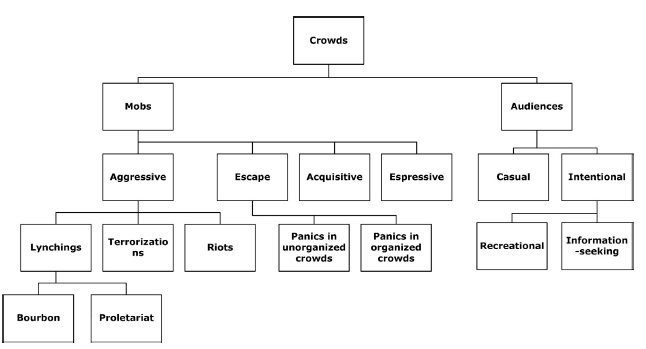
\includegraphics[width=1.0\textwidth]{BrownCrowdType}
	\caption{Brown's taxonomy of crowd (Adopted from \textcite{Pelechano2008})}
	\label{fig:brownCrowdType}
\end{figure}


According to Brown’s definition, aggressive crowds are determined by anger while escapist crowds are by fear. Acquisitive and expressive types are classified by the motivation which are acquiring objects or expressing a purpose respectively \parencite{Durupinar2010}.

\textcite{Forsyth2009} has defined a relatively similar classification of the crowd, which also distinguished a crowd into a gathering and a mob. Figure \ref{fig:forsythCrowdType} illustrates the branching of crowd classification. The difference between Forsyth’s hierarchy and Brown’s taxonomy mentioned above is that escapist and acquisitive crowds are classified under panics in Forsyth's classification. 

\begin{figure}[!htbp]
	\centering    
	\includegraphics[width=1.0\textwidth]{ForsythCrowdType}
	\caption{Forsyth's classification of crowd (Adopted from \textcite{klupfel2005models})}
	\label{fig:forsythCrowdType}
\end{figure}

The idea of using emotion, such as \textit{fear} and \textit{anger} to distinguish different types of crowds was also adopted by other sociologists \parencite{Lofland1985,Smelser1998}. Three basic fundamental emotions of humans that are \textit{fear}, \textit{joy} and \textit{anger} can express three corresponding forms of a crowd \parencite{Imhonopi2013}. Because collective behaviour is not limited by time and space, they also considered two types of crowd that are the compact crowd and the diffuse crowd, thus forming six different types of crowds (Table \ref{table:loflandCollectiveBehaviourType}). A compact crowd gathers at one particular place for the duration of a specific event whereas a diffuse crowd can be dispersed at different places and across time. An example of diffuse crowd is the collective behaviour on social media. Collective behaviour on social media might be interesting study, however, in our context of mass gathering, only compact crowds are considered to be relevant.

\begin{table}[!htbp]
	\caption{Lofland's six types of collective behaviour (Adopted from \textcite{Imhonopi2013})}
	\label{table:loflandCollectiveBehaviourType}
	\centering
	\begin{tabular}{|l|l|l|}
		\hline
		\textbf{Emotion} & \textbf{Crowd forms} & \textbf{Collective behaviour types} \\ \hline \hline
		\multirow{2}{*}{Expression of fear} & \multirow{2}{*}{Panic} & Compact \\
		& & Diffuse \\ \hline
		\multirow{2}{*}{Expression of joy} & \multirow{2}{*}{Craze} & Compact \\
		& & Diffuse \\ \hline
		\multirow{2}{*}{Expression of anger} & \multirow{2}{*}{Hostile outburst} & Compact \\
		& & Diffuse \\ \hline
	\end{tabular}
\end{table}

Elias Canetti was another author who has contributed a significant work on crowd behaviour. In ``Crowds and Power'' \parencite{Canetti1962}, he defined four physical attributes of a crowd: growth, equality, density and direction. These external characteristics of the crowd will be discussed in detail in the next section. Looking at internal aspects of the crowd, Canetti identified five prevailing emotions in the crowd which produced five different crowd types: baiting, prohibition, reversal, feast and double \parencite{McClelland2010}.

As mentioned earlier, another notable publication was the ``Understanding and planning for spectator crowds'' by \textcite{Berlonghi1995} published in public safety science. It has been brought into practice by the emergency management planners in Australia \parencite{EMA1999} and United States \parencite{FEMA2005}. Table \ref{table:berlonghiCrowdType} illustrates eleven different crowd types identified by Berlonghi. This model was also adopted in \textcite{DelirHaghighi2013a} and \textcite{Arbon2007}’s ontology for case-based reasoning to predict the patient rate in a mass gathering.

\begin{table}
	\caption{Berlonghi's eleven crowd types (Adopted from \textcite{Zeitz2009})}
	\label{table:berlonghiCrowdType}
	\centering
	\begin{tabular}{|l|p{8cm}|}
		\hline
		\textbf{Crowd type} & \textbf{Definition} \\ \hline \hline
		Ambulatory & Walking, usually calm  \\ \hline
		Disability / limited movement & Crowd has limited or restricted movement requires additional planning \\ \hline
		Cohesive / spectator & Watching a specific activity \\ \hline
		Expressive / revellous & Emotional release, for example, a cheering movement in unison \\ \hline
		Participatory & Involve in an actual event, for example, community fun runs \\ \hline
		Aggressive / hostile & Initially verbal, open to lawlessness \\ \hline
		Demonstrator & Organized to some degree, for example, pickets or marches \\ \hline
		Escaping / trampling & Danger may be real or imaginary \\ \hline
		Dense / suffocating & Reduction of individual physical movement \\ \hline
		Rushing / looting & Attempt to acquire, obtain, steal something, for example, tickets \\ \hline
		Violent & Attacking, terrorizing \\ \hline
	\end{tabular}
\end{table}

In reality, one crowd is expected to have multiple personalities \parencite{Berlonghi1995}, therefore all of the above eleven types can exist as a group in a bigger crowd. This idea was also agreed by computer scientists in their researches in crowd simulation. Their works focused on simulating the heterogeneous crowd which consists of different, independent behaviour and characteristics. Based on the Convergence Theory, the behaviour of the crowd is formed by the individuals; hence it is important to model the behaviour and interaction of the individuals in order to simulate a realistic, heterogeneous crowd behaviour \parencite{Guy2011}.

Several approaches have been proposed which were derived from the personality trait theory. This theory implied that a personality trait can influence the behaviour, emotion and mental pattern of a person \parencite{Durupinar2008}. The main objective of these researches was to map those traits with the low level parameters in simulation model to determine the behaviour of an individual agent, then observe the emerging global crowd behaviours. Two personality trait theories that were utilised are the PEN model \parencite{Guy2011} and OCEAN model \parencite{Durupinar2008,Durupinar2011}. The PEN model was constructed over three factors: Psychoticism, Extraversion, and Neuroticism while the OCEAN model consisted of Openness, Conscientiousness, Extroversion, Agreeableness and Neuroticism. The common adjectives to describe human personality were called the trait-descriptive adjectives, such as curious, alert, calm, rude were composed by different values of each of the above factors. Finally, they were mapped into corresponding parameters in the model as shown in Table \ref{table:oceanPersonality}. The simulation suggested that a low conscientiousness and agreeableness can lead to congestion during emergency evacuation and the non-conscientiousness and neuroticism was the root of panic in the crowd \parencite{Durupinar2008}.

\begin{table}[!htbp]
	\caption{Personality - trait - crowd model mapping (Adopted from \textcite{Durupinar2008})}
	\label{table:oceanPersonality}
	\centering
	\begin{tabular}{|l|l|p{6.5cm}|}
		\hline
		\textbf{Model Parameter} & \textbf{OCEAN factor} & \textbf{Personality} \\ \hline \hline
		Leadership & E, A-, C+, N & Dominant, assertive, bossy, dependable, confident, unconfident, submissive, dependent, social, unsocial \\ \hline
		Trained / not trained & O & Informed, ignorant \\ \hline
		Communication & E & Social, unsocial \\ \hline
		Panic & N, C+ & Oversensitive, fearful, calm, orderly, predictable \\ \hline
		Impatience & E+, C, A & Rude, assertive, patient, stubborn, tolerant, orderly \\ \hline
		Pushing & A, E & Rude, kind, harsh, assertive, shy \\ \hline
		Right preference & A, C & Cooperative, predictable, negative, contrary, changeable \\ \hline
		Avoidance / personal space & E & Social, distant \\ \hline
		Waiting radius & A & Tolerant, patient, negative \\ \hline
		Waiting timer & A & Kind, patient, negative \\ \hline
		Exploring environment & O & Curious, narrow \\ \hline
		Walking speed & E & Energetic, lethargic, vigorless \\ \hline
	\end{tabular}
\end{table}

\subsection{External Characteristics Modeling}

Apart from the cognitive patterns, different crowds can also be distinguished by their external or physical characteristics which can be quantitatively measured. Several features of the crowd, such as the density, movement and flow rate can be utilised to identify different crowds in the context of crowd monitoring for emergency management.

As mentioned above, \textcite{Canetti1962}’s theory also classified the crowd accordingly to their physical characteristics: growth, equality, density and direction. Each of these attributes identified a pair of crowd types. Derived from this theory, \textcite{Bandini2011} formulated six types of crowds. Open and closed crowd were defined by their growth feature. Equality and density feature determined the stagnating or rhythmic types and movement feature classified a crowd into a slow or a quick crowd. \textcite{Bandini2011} constructed an ontology approach to classify the crowd and defined a set of fuzzy rules mapping the features of the crowd with the six crowd types, as illustrated in Table \ref{table:bandiniCrowdType}.

\begin{table}[!htbp]
	\caption{Bandini's crowd type - feature mapping (Adopted from \textcite{Bandini2011})}
	\label{table:bandiniCrowdType}
	\centering
	\begin{tabular}{|p{2.3cm}|p{1.5cm}|p{1.5cm}|p{2cm}|p{2cm}|p{1.5cm}|p{1.4cm}|}
		\hline
		\textbf{Crowd features} & \textbf{Open crowd} & \textbf{Closed crowd} & \textbf{Stagnating crowd} & \textbf{Rhythmic crowd} & \textbf{Slow crowd} & \textbf{Quick crowd} \\ \hline \hline
		Physical boundary & absent & present & & & & \\ \hline
		Psychological boundary & absent & present & & present & & \\ \hline
		Movement & & & absent & present & & \\ \hline
		Density & & & high/med & low & high/med & low \\ \hline
		Growth & high & med/low & & low & high & med/low \\ \hline
		Lifespan & & & & med/short & long & short \\ \hline
		Destination & & & & near & far & near \\ \hline
	\end{tabular}
\end{table}

From transportation engineering, \textcite{Fruin1970} introduced the concept ``level of service'' to distinguish different crowds using the following features: walking speed, flow rate and restriction \parencite{Challenger2009}. This model has been adopted into the design and planning of pedestrian facilities \parencite{Shiwakoti2008,Ye2008}. Six levels of service were defined, where a higher density increased the risk of pushing, falling, crushing and trampling.

Analysing the video footages of a crowd disaster during the Hajj in 2006, \textcite{Helbing2007} claimed that the density, speed and flow of the crowd can be used as warning signs of potential accident. They coined the term ``crowd turbulence'' referring to the instabilities in the flow pattern of the pedestrians, which might trigger the trampling of people. According to their calculation, turbulence occurred when crowd pressure, which was the variance of speed multiplied by density, exceeded a certain threshold while the density of the crowd was high and the flow rate dropped below the critical threshold.

\textcite{Lee2005} also studied the causes of past crowd accidents in different countries and discovered the relationship between density and crushing and trampling. Table \ref{table:densityCrushingTrampling} explained those two types of accidents and the critical density in the crowd which could lead to each situation. This research proved that a mathematical modelling of crowd motion can identify the dangerous locations for a crowd accident, hence a careful attention to those points can minimize the risk of trampling.

\begin{table}
	\caption{Crowd density leading to crushing and trampling}
	\label{table:densityCrushingTrampling}
	\centering
	\begin{tabular}{|l|p{9.5cm}|l|}
		\hline
		\textbf{Accident type} & \textbf{Definition} & \textbf{Density} \\ \hline \hline
		Trampling & High density with possible movement. Fatalities are caused by falling and being trampled & 5 ped/m2 \\ \hline
		Crushing & Extremely high density with almost impossible movement. Fatalities are caused by being compressed by pressure & 10 ped/m2 \\ \hline
	\end{tabular}
\end{table}

As mentioned in the previous section, crowd density was often used as a measure to monitor the safety of the crowd. Different crowds were classified by the level of density in the works by \textcite{Marana1997} and \textcite{Weppner2013} starting from very low density to very high density.

\subsection{Analysis and Discussion}

Psychological models \parencite{Blumer1951,Lofland1985,Momboisse1967} were able to describe different crowd types based on the psychosocial domain of the crowd. Because reasoning was not clearly defined in those models, it would depend on the interpretation of the observers to determine whether a particular crowd type would pose a potential danger. This requires previous domain knowledge and experience that limit its use to the domain experts.

Simulation models using PEN \parencite{Guy2011} and OCEAN \parencite{Durupinar2008} personality trait theory were able to identify which personality of an individual can cause problems in evacuation. However, measuring individual’s personality is a difficult task.

Case-based reasoning in DO4MG \parencite{DelirHaghighi2013a} considered both the psychological features and physical features of a crowd to predict the emergency situation. Case-based reasoning in general relied on historical data for prediction, therefore applying this method in crowd monitoring would be challenging when there is no access to similar data and some information required in the ontology cannot be captured in real-time.

The classification of crowd proposed by \textcite{Lofland1985} and \textcite{Smelser1998} suggested the importance of emotion as the motivation of the behaviour of a crowd. This idea was also agreed by \textcite{Brown1954} whose taxonomy also used \textit{anger} and \textit{fear} to categorise the crowd.

Most of models which were capable of predicting the critical situations were based on the external characteristics of the crowd such as the density, size or movement \parencite{Helbing2007,Lee2005}. This information can be obtained by sensors and the prediction can be made by quantitative reasoning. However, these models did not emphasise on the psychosocial factors which are important in emergency management.

\textcite{Berlonghi1995}’s model has been broadly adopted as the guideline in emergency management. Comparing this model with other works from such authors as \textcite{Blumer1951} or \textcite{Momboisse1967}, it can be noticed that Berlonghi's model is also capable of representing the crowd types defined in other models. 

\begin{center}
	\begin{longtable}{|p{2.2cm}|p{2cm}|p{2cm}|p{4.2cm}|p{2.8cm}|}
	\caption{Comparison of different Crowd Models}
	\label{table:crowdModelComparison} \\
	\hline
	\multirow{2}{\linewidth}{\textbf{Crowd type}} & \multicolumn{3}{c|}{\textbf{Origin}} & \multirow{2}{\linewidth}{\textbf{Example}} \\
	\cline{2-4}
	& Crowd type & Source & Definition & \\
	
	\hline \hline
	\multirow{2}{\linewidth}{Ambulatory crowd} & Ambulatory \newline \newline & \textcite{Berlonghi1995} & \multirow{2}{\linewidth}{People are walking in and out or to and from a venue \parencite{Berlonghi1995}. Usually calm movement \parencite{Zeitz2009}} & \multirow{2}{\linewidth}{People entering a stadium or a concert} \\
	\cline{2-3}
	& Casual crowd \newline & \textcite{Blumer1951} & & \\

	\hline
	\multirow{2}{\linewidth}{Limited movement crowd} & Disability / Limited movement \newline \newline & \textcite{Berlonghi1995} & \multirow{2}{\linewidth}{People are limited or restricted in movement \parencite{Berlonghi1995}. People have loose connection and little interaction \parencite{Blumer1951}. People happen to be at a given place but not unified or organized \parencite{Momboisse1967}} & \multirow{2}{\linewidth}{People waiting in a queue to get tickets} \\
	\cline{2-3}
	& Casual crowd \newline \newline \newline & \textcite{Blumer1951} & & \\

	\hline
	\multirow{2}{\linewidth}{Crowd of spectators} & Cohesive / Spectators \newline \newline \newline & \textcite{Berlonghi1995} & \multirow{2}{\linewidth}{People are present to watch a specific event, not to communicate with each other. Characterized by the desire to stay and watch \parencite{Berlonghi1995}. People are assembled for a specific purpose \parencite{Blumer1951}} & \multirow{2}{\linewidth}{People watching a football game in the stadium or catching a concert in a theatre} \\
	\cline{2-3}
	& Conventional crowd \newline \newline \newline & \textcite{Blumer1951} & & \\

	\hline
	\multirow{2}{\linewidth}{Participatory crowd} & Participatory & \textcite{Berlonghi1995} & \multirow{2}{\linewidth}{People are involved in actual activities of an event \parencite{Berlonghi1995}} & \multirow{2}{\linewidth}{People walking in a parade} \\
	\cline{2-3}
	& Conventional crowd & \textcite{Blumer1951} & & \\

	\hline
	\multirow{3}{\linewidth}{Expressive crowd} & Expressive / revellous & \textcite{Berlonghi1995} & \multirow{3}{\linewidth}{People are involved in an emotional release \parencite{Berlonghi1995}} & \multirow{3}{\linewidth}{People cheering, chanting in unison. Human wave in a soccer match} \\
	\cline{2-3}
	& Expressive crowd & \textcite{Blumer1951} & & \\
	\cline{2-3}	
	& Expressive crowd & \textcite{Momboisse1967} & & \\	

	\hline
	\multirow{2}{\linewidth}{Aggressive crowd} & Aggressive / Hostile & \textcite{Berlonghi1995} & \multirow{2}{\linewidth}{People are verbally assaultive and showing disregard \parencite{Berlonghi1995}} & \multirow{2}{\linewidth}{Soccer hooligan shouting} \\
	\cline{2-3}
	& Hostile or aggressive crowd & \textcite{Momboisse1967} & & \\

	\hline
	\multirow{2}{\linewidth}{Crowd of demonstrators} & Demonstrator \newline \newline & \textcite{Berlonghi1995} & \multirow{2}{\linewidth}{People are organized by an established leadership for specific reason \parencite{Berlonghi1995}. A crowd which has some political goal \parencite{Imhonopi2013}} & \multirow{2}{\linewidth}{A protest, a picket} \\
	\cline{2-3}
	& Protest crowd & \textcite{McPhail1983} & & \\

	\hline
	\multirow{4}{\linewidth}{Escaping crowd} & Escaping / Trampling & \textcite{Berlonghi1995} & \multirow{4}{\linewidth}{People are trying to escape from a danger or a threat \parencite{Berlonghi1995, Momboisse1967}} & \multirow{4}{\linewidth}{A evacuation from a fire} \\
	\cline{2-3}
	& Escapist mob & \textcite{Blumer1951} & & \\
	\cline{2-3}	
	& Trampling & \textcite{Hughes2009} & & \\
	\cline{2-3}
	& Acting crowd & \textcite{Blumer1951} & & \\

	\hline
	\multirow{2}{\linewidth}{Crushing crowd} & Dense / Suffocating \newline \newline & \textcite{Berlonghi1995} & \multirow{2}{\linewidth}{People have limited individual movement \parencite{Berlonghi1995} and being compressed. Characterized by high density \parencite{Lee2005}} & \multirow{2}{\linewidth}{A human stampede at new year festival} \\
	\cline{2-3}
	& Crushing & \textcite{Lee2005} & & \\

	\hline
	\multirow{3}{\linewidth}{Rushing / Looting crowd} & Rushing / looting & \textcite{Berlonghi1995} & \multirow{3}{\linewidth}{People are trying to obtain or steal something \parencite{Berlonghi1995}} & \multirow{3}{\linewidth}{People looting food after a natural disaster} \\
	\cline{2-3}
	& Acquisitive mob & \textcite{Momboisse1967} & & \\
	\cline{2-3}	
	& Acting crowd & \textcite{Blumer1951} & & \\	

	\hline
	\multirow{3}{\linewidth}{Violent crowd} & Violent & \textcite{Berlonghi1995} & \multirow{3}{\linewidth}{People are attacking and rioting with disregard for laws and rights \parencite{Berlonghi1995}} & \multirow{3}{\linewidth}{A riot in Ferguson, USA} \\
	\cline{2-3}
	& Aggressive mob & \textcite{Momboisse1967} & & \\
	\cline{2-3}	
	& Acting crowd & \textcite{Blumer1951} & & \\	

	\hline
	\end{longtable}
\end{center}

Table \ref{table:crowdModelComparison} summarises the comparison between different crowd models using Berlonghi's model as the baseline. This suggests the potential to incorporate Berlonghi's crowd types as the standard crowd model for crowd monitoring. On the other hand, there is some challenges adopting Berlonghi's model into a crowd monitoring approach. There is overlapping in the definition of crowd types. For example, it is difficult to distinguish the difference between a hostile and a violent crowd. Furthermore, in this model, the crowd types were only defined by their gathering purposes and activities in the crowd. There is a lack of additional features and attributes for an automated classification to be provisioned. Therefore, in order to incorporate Berlonghi's model into crowd monitoring, the crowd types must be refined and introduced with additional features, such as emotion as suggested by \textcite{Lofland1985} and \textcite{Smelser1998}. The idea of forming a hierarchical structure \parencite{Brown1954,Forsyth2009} is considerable as similar types can be grouped together and the classification can be done in different levels.

\section{Findings}
From the analysis of the state-of-the-art crowd monitoring techniques, following limitations and gaps can be noticed:
\begin{inparaenum}[i)]
	\item the limitation of vision-based and mobile sensing approaches;
	\item despite the great potential, very limited work has been done using social media as the information source in crowd monitoring;
	\item the lack of a standard crowd model in existing crowd monitoring techniques
\end{inparaenum}.

Our literature review on existing crowd models also shows several findings:
\begin{inparaenum}[i)]
	\item the potential to use broadly adopted \textcite{Berlonghi1995}'s models as the standard crowd model for crowd monitoring;
	\item the need to introduce additional features to distinguish different crowd types in Berlonghi's model;
	\item the impact of emotion on the behaviours of the crowd
\end{inparaenum}.

\section{Conclusion}
This chapter has analysis the strength and limitation of the state-of-the-art crowd monitoring techniques using image processing, sensory data analysis and social media analysis. Our literature review has showed the potential of using social media as the information source for context data in crowd monitoring.

Our analysis also has covered the existing crowd models in the literature from a wide range of research areas. It shows the potential to adopt \textcite{Berlonghi1995}'s model as the standard crowd model in crowd monitoring as well as the need to introduce additional features into the model to distinguish different crowd types.
% !TEX root = ../thesis.tex
\chapter{Approach}
\label{ch:approach}
% **************************** Define Graphics Path **************************
\ifpdf
\graphicspath{{Chapter3/Figs/Raster/}{Chapter3/Figs/PDF/}{Chapter3/Figs/}}
\else
\graphicspath{{Chapter3/Figs/Vector/}{Chapter3/Figs/}}
\fi

\section{Introduction}
\label{sec:approachIntro}
Despite the importance of crowd monitoring in mass gathering events, the literature review in the previous chapter has identified several gaps in the research, especially in crowd modelling. Most state-of-art crowd monitoring techniques do not incorporate a typology to identify and distinguish different types of crowd. In other words, they lack the capability to make distinction of different crowd types that can occur in a mass gathering event. To address this issue, our proposed approach employs one of the most famous existing works on definition of crowd types in emergency management - the \citet{Berlonghi1995}'s model. Our approach also automates the classification of crowd type by considering the emotional conditions of the crowd. Those novelty attempts are integrated into a complete framework for real-time crowd monitoring, which will be discussed in detail in this chapter.

This chapter is structured as follow. Firstly, the overview of our proposed crowd monitoring framework will be introduced. Then each component in the framework will be discussed in the following sections. The chapter ends with the conclusion which will give a summarised look at the framework.

\section{An Overview of the Crowd Monitoring Framework}

The literature review in Chapter \ref{ch:litReview} has summarised that most of the state-of-art crowd monitoring approaches are focusing on using computer vision to automate the analysis of CCTV system. The literature review has revealed several limitations of the computer vision technique, such as the effect of obstacles and low lighting condition. With the rapid development of mobile computing and the increasing popularity of mobile devices, mobile sensing seems to be a more potential technique to collect contextual data for crowd monitoring, for example GPS receivers and accelerometers. Context data refers to all the knowledge that is related to a crowd. Context data can be at raw level such as the acceleration and rotational forces generated by accelerometer built in a participant's mobile phone, or at high level such as the current activity that the user is performing using activity recognition techniques.

Apart from the ``hard sensors'' where physical sensors are used, the literature review also highlights that another type of information source known as the ``soft sensor'' can be used to monitor the crowd and detect the occurrence of stampede in a crowd which is the social media \citep{Ramesh2014}. The use of social media analysis for crowd monitoring has been introduced in a related work by \citet{DelirHaghighi2013}. It has the great advantage of feasibility as it only relies on the software and no additional hardware is required to be installed. Despite this strength, our literature review shows that very limited works have been done to utilize social media to support crowd monitoring in emergency management.

Secondly, another finding from the literature review is that the actual behaviour of a crowd depends largely on the emotions of the participants \citep{Kornblum2011, jasper2011emotions}. For that reason, it is essential for a crowd monitoring approach to consider the influence of emotions in the crowd. Although human emotion is an abstract concept and very difficult to measure with ``hard sensors'', it is possible to capture the emotion of a person from the verbal expressions, such as text \citep{alm2005emotions} or speech \citep{sobin1999emotion}. This is where social media further proves its advantage over the ``hard sensors''. By applying analysis on the social media, we can capture the emotions in a crowd, thus enabling the inference of the crowd's condition. For that reason, this project will propose a crowd monitoring framework that employs the emotion analysis of social media to support emergency management in mass gatherings by determining the current type of the crowd. 

Finally, the literature review also reveals another gap in the research that is the limitation of the crowd modelling employed in crowd monitoring approaches. Most existing crowd monitoring techniques do not base on any crowd model which can distinguish between different crowd types and identify the exact crowd type that is happening without the interpretation of human. By exploring broader into other disciplines, our literature review points out several notable works on crowd modelling and classification in the police literature and public safely science. Among those works, \citet{Berlonghi1995}'s work stands out as the most commonly adopted model by the emergency management bureaus worldwide. Our proposed crowd monitoring framework is established on the \citet{Berlonghi1995}'s model which consists of eleven different crowd types. Yet, a systematic approach to classify one crowd into those types is challenging because \citet{Berlonghi1995}'s model only describes the crowd types and there is no attribute or method defined in the existing model to make the distinction between them. Therefore, in our approach, we would like to propose a mapping model that connects the emotion model with the crowd model, enabling the fuzzy classification of crowd type by emotions. The reason fuzzy logic is utilized in our approach is because of its capability of representing multiple truths rather than the absolute true or false like in classical logic. It is difficult to divide people in a mass gathering into very distinct classes using rule-based reasoning since crowd types can be overlapping. Fuzzy logic is able to calculate the degree of membership of each crowd type in a particular crowd and represent the real-time and gradual changes in crowd type.

In conclusion, our proposed approach will address the gaps that are identified in the previous chapters by: 
\begin{inparaenum}[i)]
\item incorporating social media as the information source for context data;
\item capturing the emotions of a crowd by analysing the context data from soft sensors;
\item identifying the type of a crowd by applying fuzzy rule based inference to the crowd emotions
\end{inparaenum}. These objectives can be integrated together in a complete process as illustrated by Figure \ref{fig:processOverview}. Social media is firstly probed to get the context data at the raw level. This raw data is then processed in an emotion analysis to extract high level context data, that is the emotional states of the crowd. These emotional states are in turn used as the attributes or features to classify a crowd into a specific type.

\begin{figure}[htb!] 
\centering    
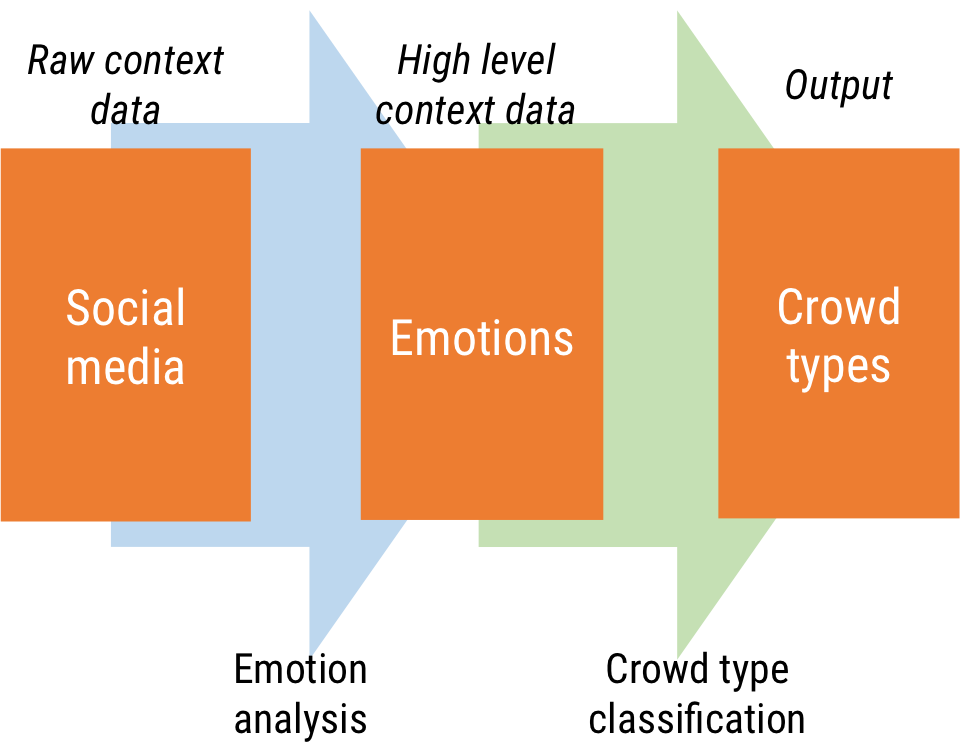
\includegraphics[width=0.5\textwidth]{ProcessOverview}
\caption{A process to identify a crowd type from social media}
\label{fig:processOverview}
\end{figure}

From the functional point of view, the process can be implemented into a framework. Figure \ref{fig:frameworkOverview} shows our framework consisting of following components:
\begin{inparaenum}[i)]
\item Context data;
\item Emotion analysis;
\item Emotion model;
\item Crowd model;
\item Emotion - Crowd type mapping model;
\item Rule based reasoning
\end{inparaenum}. Each component will be discussed further in the sections below.

\begin{figure}[htb!] 
\centering    
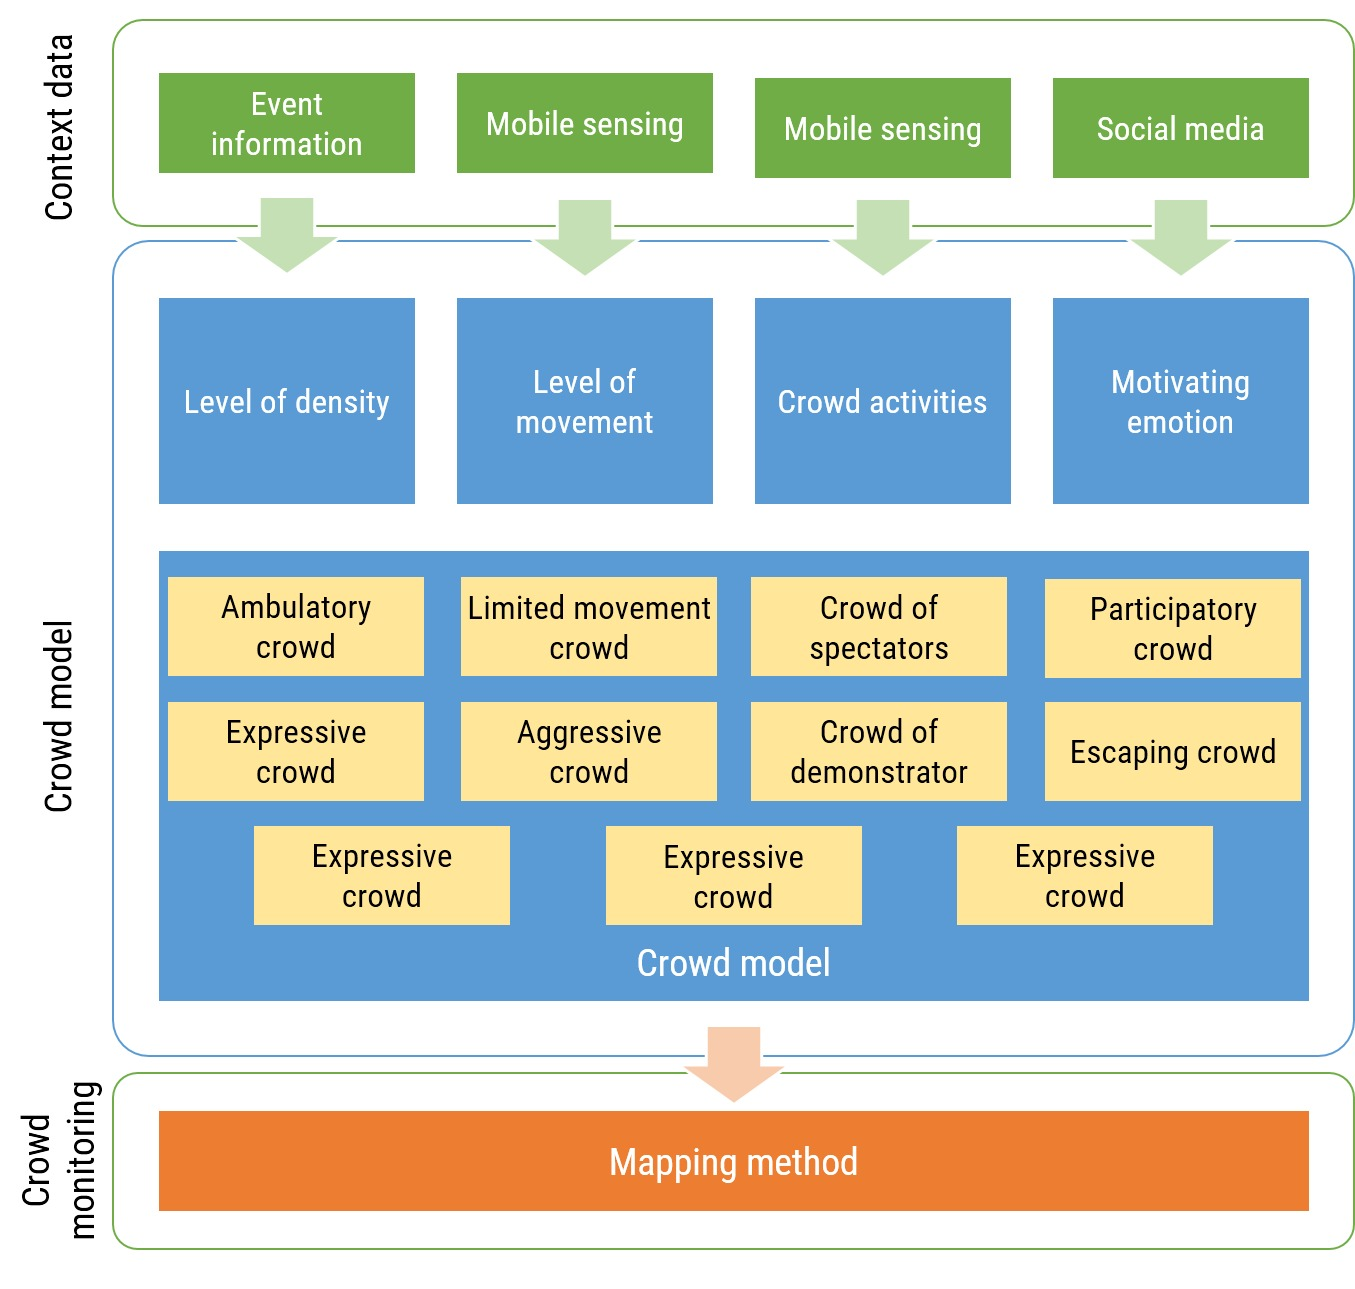
\includegraphics[width=1.0\textwidth]{FrameworkOverview}
\caption{An overview of the crowd monitoring framework using emotion analysis of social media}
\label{fig:frameworkOverview}
\end{figure}

\section{Context Data}
The first component of the framework is the Context Data component. In our proposed framework, contextual data is gathered from the social media as the information source. Social media is the generic term referring to a wide range of Internet based tools that enable a user to create and share information with each other \citep{kaplan2010users}. These tools include social network services such as Facebook and Twitter, blogs, Internet forums and channels which have marked the beginning of Web 2.0. Unlike other traditional media such as newspaper or television, the content on social media is created by the users, or also known as user-generated content \citep{kaplan2010users}. User-generated content can be in various formats such as text, image or video. Because of the fact that the content is being generated by the users themselves, social media is an effective source to obtain the knowledge about the users. In our domain and application of crowd monitoring, the kind of knowledge that is important to capture is the emotional state of the participants in the crowd. 

In our research, we will focus on the use of social media, or Twitter in particular, as the information source for context data, because of the following reasons. Firstly, among social media, Twitter is the most commonly used in researches because of its large volume of users and its public APIs which make the data highly accessible. The user-generated content is mostly text-based and in the form of a short message which has no more than 140 characters called tweet. Because of this length limit, a tweet is usually very simple in term of the meaning and each tweet focuses on expressing the idea of the author on one particular topic. This fact makes the a semantic analysis of tweets more feasible in real-time than other content, for example, a long blog article.

A tweet might also contain information beyond the text. A significant number of tweets are geo-tagged, which means they are attached with the location information when they are posted to Twitter. This location information can be in the form of exact coordinates if the user posts the tweet from a GPS enabled mobile phone. Alternatively, this location might also be a relative location such as point of interests or town if the user checks in or attaches a place with the tweet.

Another useful information that might exist in a tweet is hashtags. Hashtags are created by the users, and usually are put in a tweet to refer to the topic that is mentioned in the tweet \cite{mohammad2014using}. In some mass gathering events such as the Australia Open or music festivals, there are pre-defined hashtags created for these particular events so that a user can put the hashtags into his tweet when mentioning about the events. Similarly to the geo-location, this information can also be used to filter for tweets belonging to a specific event.

Finally, using Twitter as the information source for crowd monitoring has some certain advantages. Firstly, the data can be collected in real-time, enabling the real-time monitoring which is an essential operation in emergency management because of the dynamic nature of a crowd that it can change from a calm type to an aggressive type \citep{Berlonghi1995}. Secondly, it does not require any pre-installed hardware or software on the participants, which increases the feasibility of our proposed framework.

\section{The Emotion Model}

From the literature review, a crowd type can be described as a form of collective behaviour of a group of people in close proximity. The other form of collective behaviour is mass which involves people dispersed in a large area and does not belong to our context of emergency management in mass gathering. Both the Convergence Theory and the Emergent Norm Theory \citep{mcphail1991myth} support the idea that a crowd behaviour is formed by people with a common motivation. In our framework, we emphasize on the emotional factor as the common motivation of the behaviour in the crowd. Different emotions can consequently lead to different crowd behaviours. For example, according to Lofland's typology of spontaneous collective behaviours \citep{Kornblum2011}, a panic exodus from burning theatre is motivated by the fear whereas a race riot is aroused by the anger. Therefore, an emotion model is essential to distinguish different emotions of the people in the crowd.

Human emotion is no doubt complex and confusing \citet{plutchik2001nature}. Therefore, it is difficult even to just list all emotions, not to mention modelling them. However, it is often assumed among theories of emotions that there exists a small set of basic or fundamental emotions, yet there is still little agreement on the number of basic emotions and what emotions are in the list \citep{Ortony1990}. Based upon the theory of evolution of the biological process, \citet{plutchik2001integration} was able to identify eight basic emotions consisting of four pairs of opposite emotions: anger/fear, joy/sadness, trust/disgust, anticipation/surprise. Investigating the facial expression of human, \citet{ekman1971constants} suggested there are six basic emotions that can be universally recognised, regardless of the language. The six basic emotions are anger, fear, happiness, sadness, surprise and disgust as illustrated in Figure \ref{fig:emotionModel}. Ekman's model has been adopted in many researches regarding human emotions \citep{mohammad2014using, roberts2012empatweet, alm2005emotions}. 

\begin{figure}[htb!]
\centering    
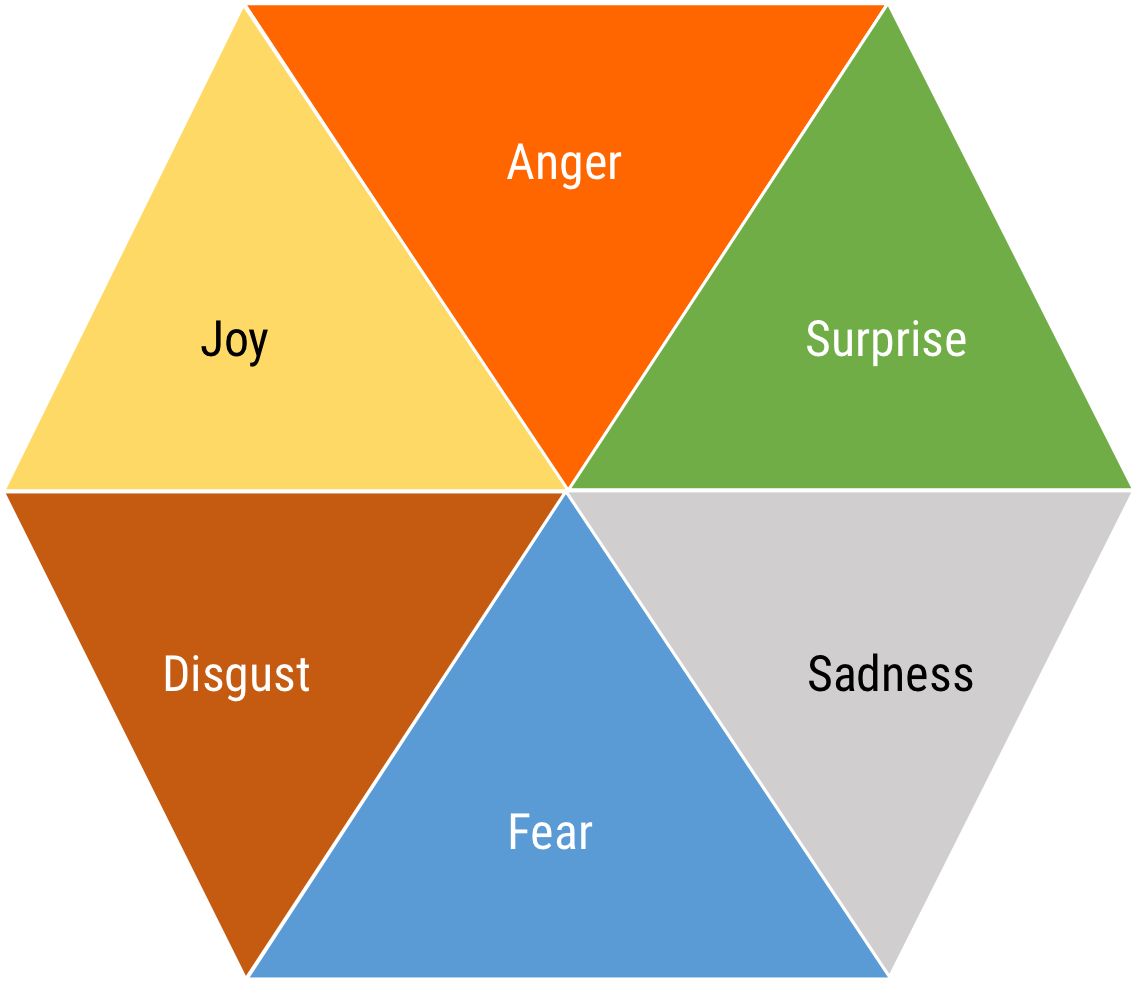
\includegraphics[width=0.5\textwidth]{EkmanModel}
\caption{Ekman's six basic emotions}
\label{fig:emotionModel}
\end{figure}

A recent research by \cite{Jack2014} has pointed out the similarity during the early signal of the facial expression between anger and disgust, as well as surprise and fear. For example, both anger and disgust share a wrinkled nose, while both surprise and fear share raised eyebrows. Based on these findings, they suggest only four basic emotions. The reduction in the number of basic emotions effectively simplifies the complexity of our emotion model. Therefore, the four most basic emotions consisting of anger, fear, happiness and sadness will be adopted as our emotion model in the proposed framework.

\section{Emotion Analysis of Social Media}

A recent analysis on the content on Twitter reveals that the users are using Twitter for a variety of purposes, which can be grouped in two main types: updating their statuses or sharing information \citep{java2007we}. Regardless of the content in both cases, a tweet often conveys the author's emotional status \citep{bollen2009modeling}. By capturing the emotion expressed in the text, it is possible to infer the emotional state of the author. In our framework, as can be seen from Figure \ref{fig:processOverview} a tweet can be considered as a raw context data collected from the information source whereas the emotion in the tweet is the high-level context data that is inferred and it will be used in our proposed crowd type classification. This transformation from the raw-level to the high-level context data is performed by the Emotion Analysis component.

Regarding emotion detection from tweets, there have been several related works such as from \citet{bollen2009modeling}, EmpaTweet by \citet{roberts2012empatweet} and NRC Hashtag Emotion from \citet{mohammad2014using}. The common approach that was employed in these works is the Bag-Of-Words model which only considers the occurrence of words while ignoring the grammar and meaning. \citet{bollen2009modeling} used an extended version of the Profile of Mood States with 765 terms from 65 mood adjectives and mapped a tweet into one of the six moods: tension, depression, anger, vigour, fatigue and confusion.

The EmpaTweet by \citet{roberts2012empatweet} collected tweets on 14 selected topics that each topic was expected to evoke a particular emotion in seven emotions: \textit{anger}, \textit{disgust}, \textit{fear}, \textit{joy}, \textit{sadness}, \textit{surprise} and \textit{love}. The collected tweets formed the labelled corpus which was used to train a classifier to automatically detect the emotions from Twitter.

Using the hashtags, the NRC Hashtag Emotion by \citet{mohammad2014using} collected the tweets which were attached with these emotional hashtags: \#anger, \#disgust, \#fear, \#joy, \#sadness and \#surprise and their synonyms. These hashtags served as the label of a tweet, which annotated the emotion in the tweet. The experiment also verified that the self-labelled hashtags were consistent and matched with the annotation by trained judges. 


Another notable corpus is the NRC Hashtag Emotion corpus, in which tweets are collected by emotion-word hashtags corresponding to Ekman's six emotions: \#anger, \#disgust, \#fear, \#joy, \#sadness and \#surprise and their synonyms \citep{mohammad2012emotional}. The approach used in NRC Hashtag Emotion corpus appears to be more robust as it relies on the self-labelled emotions by the authors rather than the topic-based emotion assumption like in EmpaTweet. The evaluation also verifies that the self-annotated emotions eventually match the emotions annotated by the judges

Our proposed method is based on a combination of Bag-of-Word model, weighting and a simple voting scheme, which will be discussed in the next sections.

\subsection{Bag-of-Word Model}
Bag-Of-Word model is a simple representation of a document which only considers at the frequency of appearance of the words in a document while disregarding the grammar and the order of the words. In our research using Twitter as the corpus, a document is a single tweet and a word is an uni-gram word building up the tweet. The process that splits a document into a sequence of words is called tokenizer. In our experiment which will be mentioned in Chapter \ref{ch:eval}, the Stanford NLP Tokenizer \footnote{http://nlp.stanford.edu/software/tokenizer.shtml} is applied to tokenize a tweet into words and also to filter out data that is not in our interest, such as URLs and emoticons. 

\begin{figure}[htb!] 
\centering    
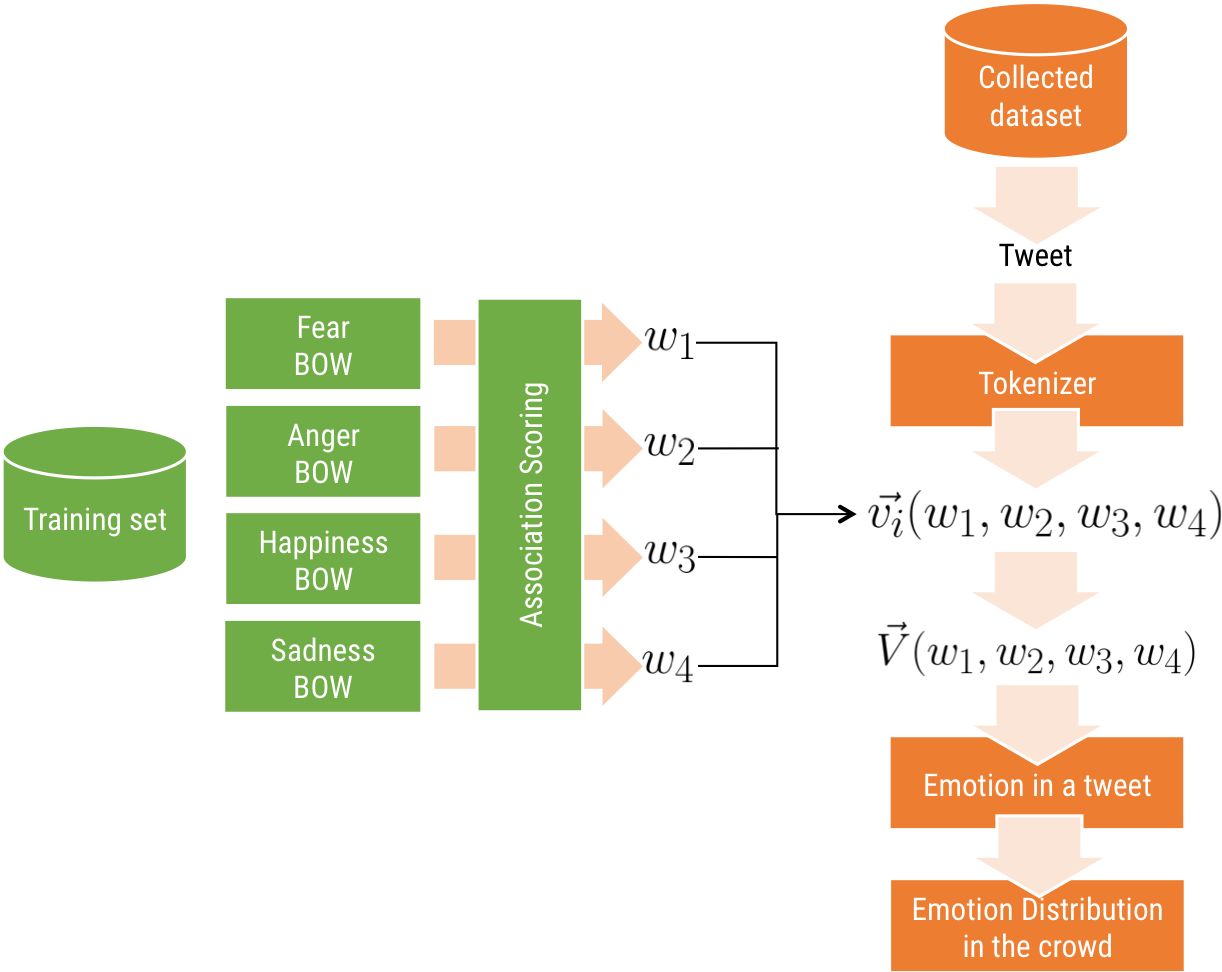
\includegraphics[width=0.75\textwidth]{BagOfWord}
\caption{An example of a tweet tokenized into words}
\label{fig:bagOfWord}
\end{figure}

In the Bag-Of-Word representation (Figure \ref{fig:bagOfWord}), the number of occurrence of a word in the tweet contributes to its significance in the tweet. For example, if a word appears twice in the tweet, it will have a doubled weight compared with words with single appearance, thus being more significant. 

The weight of a word represents its association with a specific emotion from the list of four basic emotions mentioned above. Therefore, a word will have four weight scores for each emotions: anger, fear, happiness, sadness, which can be illustrated by a proposed ``emotional weight vector'' with four dimensions corresponding to the four emotions. 
\[
	\vec{v_i}(v_1, v_2, v_3, v_4)
\] where \(v_i\) is an emotional weight vector of a word and \(v_{1...4}\) are four dimensions that represent the four emotions.

In conclusion, using the Bag-Of-Word approach, we can consider that a tweet consists of a series of words, each of which has its association with the four emotions, which is described by an emotional weight vector. The next section will discuss the method to to calculate the ``emotional weight vectors'' \(\vec{v_i}\) of the words and identify the dominating emotion in a tweet.

\subsection{Emotion Word Corpus and Emotional Weight Vector}
Our emotion analysis can be considered as a supervised classification of emotion for a tweet. The analysis requires a collection of words to be gathered and the ``emotional weight vector'' \(\vec{v_i}\) of each word in the collection must be calculated accordingly. Such collection is often referred as the corpus. In order for the calculation of ``emotional weight vector'' to be performed, a corpus of tweets that have been labelled with a correct emotion for each tweet is necessary.

Emotion analysis from text is not a new topic in the field of natural language processing. There have been a number of works regarding the construction of text-emotion corpus from various sources such as mails \citep{mohammad2011tracking} and books \citep{mohammad2011once}, newspaper headlines \citep{strapparava2008learning}. Those proposed corpora can be integrated into our framework. However, the language used in a tweet can be significantly different from other text content because of the difference in the usages that a tweet is limited to 140 characters in length and the users mostly use Twitter to update on themselves or to share information. Therefore, only the corpora that are built from Twitter will be of interest to the our crowd monitoring framework.

EmpaTweet proposed by \citet{roberts2012empatweet} is a corpus on Twitter that is annotated with seven emotions: anger, disgust, fear, joy, love, sadness and surprise. Those emotions are taken from Ekman's set of basic emotions plus love as the seventh emotion. The tweets are collected in 14 topics which are chosen in a manner that each topic is expected to evoke a particular emotion in the tweets. Another notable corpus is the NRC Hashtag Emotion corpus, in which tweets are collected by emotion-word hashtags corresponding to Ekman's six emotions: \#anger, \#disgust, \#fear, \#joy, \#sadness and \#surprise and their synonyms \citep{mohammad2012emotional}. The approach used in NRC Hashtag Emotion corpus appears to be more robust as it relies on the self-labelled emotions by the authors rather than the topic-based emotion assumption like in EmpaTweet. The evaluation also verifies that the self-annotated emotions eventually match the emotions annotated by the judges. Because of this robustness, the NRC Hashtag Emotion corpus is selected as the emotion word corpus in our emotion analysis. The corpus has approximately 21000 tweets and 14000 words.

From the NRC Hashtag Emotion corpus, \citet{mohammad2012emotional} also calculates the association of each word with each of the \citet{ekman1971constants}'s six emotions, which is called Strength of Association (SoA), based on the frequency of occurrence of this word in tweets labelled with a specific emotion. The score is from 0 indicating no association to infinity indicating maximum association. The result is a word emotion lexicon which list all words in the corpus with theirs SoA with the six emotions. This lexicon has been made available to use for research purposes \footnote{http://saifmohammad.com/WebPages/lexicons.html}. In the NRC Hashtag Emotion Lexicon version 2.0, the SoA is calculated to Plutchik's eight emotions. Because the eight emotions proposed by Plutchik also include anger, fear, happiness (joy) and sadness, this lexicon can be used in our calculation of the ``emotional weight vector'' \(\vec{v_i}\). The four dimensions of the vector are equivalent to the four emotions, and in each dimension the magnitude of the dimensional vector represents the SoA to the corresponding emotion.

From the weight vectors of the words in a tweet, the dominating emotion depicted in the tweet can be determined using a simplified voting system which will be discussed in the following section.

\subsection{Voting System and Dominant Emotion}
Because a word can have the different weights in the four emotions, consequently a tweet consisting of a set of words also has the association with the four emotions. It can be notated as a vector that is summation of the weight vectors of the words building up the tweet.
\[
	\vec{V} = \sum_{i=1}^{n} \vec{v_i}(v_1, v_2, v_3, v_4)
\]
where \(\vec{V}\) is the summative weight vector of the tweet, \(\vec{v_i}\) is a weight vector of one word and \(n\) is the total number of words in the tweet.

Although a tweet might be associated with all four emotions, one specific emotion is expected to dominate the whole tweet. In order to extract the dominating emotion in a tweet, following voting system that can interpret the vector is proposed as follow. An ``emotional weight vector'' \(\vec{v_i}\) can be considered as a vote cast by a word that indicates how strongly the word agrees with each emotion. Similarly, the summative vector \(\vec{V}\) can be interpreted as the overall result of the voting, which illustrates how close the whole tweet is from each emotion. The dominant emotion can then be determined by the highest vote from the voters. In other words, the dimension that has the largest magnitude will be selected as the dominant emotion in the tweet.

\subsection{Emotions in the Crowd}
As illustrated by Figure \ref{fig:processOverview}, the tweets collected in the first stage of the process provides the context at the raw-level about a crowd in a mass gathering. By performing the emotion analysis, the dominant emotion in each tweet can be extracted. This emotion in fact represents the emotion of an individual in the crowd rather than the crowd as a whole. The relationship between individual emotion and group emotion has been discussed in several researches. \citet{barsade1998group} suggest the top-down approach that the group emotion can arise and felt by individual member, while at the same time, in a bottom-up manner the group emotion can be shaped by the compositional effects of individual emotions. This theory confirms the possibility to represent the crowd emotion as whole from the individuals' emotion.

Because of the fact that people with different emotional state can exist in one crowd, we introduce the fuzziness to the representation of emotions in a crowd. The fuzziness allows a crowd to have multiple emotions with a different degree of membership toward each emotion. To measure the degree of membership of a crowd to a specific emotion from the individual emotion of the participants, we propose following method. The degree of membership of a crowd's emotion to emotion \(e_i\) at a given period \(t\) is calculated by below formula.
\[
	\forall e_i \in \{anger, fear, happiness, sadness\}: d(e_i)_t = \frac{n(e_i)_t}{N_t}
\]
where \(d(e_i)_t\) is the degree of membership toward emotion \(e_i\), \(N_t\) is the total number of data sampled during \(t\) and \(n(e_i)_t\) is the number of data classified with emotion \(e_i\) among \(N_t\).

This degree of membership \(d(e_i)\) can have any value from 0 to 1, indicating the how close the emotion of the crowd is to \(e_i\) at specific time period \(t\). The calculation of the degrees of membership is performed repetitively with an interval which allows us to detect the change of emotional state of the crowd. The value of \(t\) has influence on the sensitivity of the detection and depends on the sampling rate.

\section{Crowd Model}

The ultimate objective of our crowd monitoring framework is to identify the type of a crowd. Therefore, a crowd model that can describe and differentiate different crowd types is required. From the emergency management point of view, the literature review highlights \citet{Berlonghi1995}'s model as one of the most significant works on crowd types. As mentioned in Chapter \ref{ch:litReview}, \citet{Berlonghi1995} has identified eleven different types of crowd in mass gathering. Each crowd type is described by the movement, participation and behaviour \citep{Zeitz2009}. \citet{Berlonghi1995}'s definition has been widely adopted as the guideline by the emergency bureaus in Australia \citep{EMA1999} and USA \citep{FEMA2005}. Eleven types of crowd are described as below.
\begin{itemize}
\item \textbf{Ambulatory crowd} - is a crowd walking in and out of a venue, to and from parking areas or walking to use restroom or concession facilities.
\item \textbf{Disability/limited movement crowd} - is a crowd of people that in some way are limited or restricted in their movement. Their level or lack of ability to walk, see, hear or speak may require more planning than is provided for all other spectators.
\item \textbf{Cohesive/spectator crowd} is a crowd watching the activities of an event or at the scene of an accident. Its primary character is the fact that people are interested in watching something specific that they came to see.
\item \textbf{Expressive/revellous crowd} - is one involved in some sort of an emotional release which can include cheering, movement in unison, celebrating, dancing, chanting or singing.
\item \textbf{Participatory crowd} - is the crowd of people involved in the actual activities of an event. Sometimes these people may be professional performers or athletes. At other times the people attending the event are participating in an actual sport, such as a marathon. Children may go up onto a stage to perform at the invitation of professional performers.
\item \textbf{Aggressive/hostile crowd} - is one that is becoming verbally aggressive towards or disregarding the instructions of ticket takers, ushers or security personnel. This crowd can get threateningly rowdy and is very open to lawlessness.
\item \textbf{Demonstrator crowd} - is one that is organised to some degree by some established leadership and whose actions may include picketing, marching, chanting or demonstrating at a particular location for a specific purpose.
\item \textbf{Escaping/trampling crowd} - is one that is attempting to escape from danger either of an actual or imagined threat to life. This includes a crowd involved in an organised evacuation procedure and a panic mob pushing and shoving with no order whatsoever.
\item \textbf{Dense/suffocating crowd} - is one in which individual physical movement is rapidly becoming less likely or impossible due to the density of the crowd. People are attempting to move,but they are either swept along with the movement of the crowd or are falling on top of each other. The results of this compression of people are fatalities and serious injuries due to suffocation.
\item \textbf{Rushing/looting crowd} - is one whose principal purpose is to obtain, acquire or steal something. This includes rushing to get the most preferred seats, autographs or actually stealing property. This very often results in fatalities, serious injuries and considerable property damage.
\item \textbf{Violent crowd} - is a crowd that is attacking, terrorising and rioting with complete disregard for laws and the rights of others.
\end{itemize}
However, relying only on the description, it is difficult to make distinct of different crowd types without human observation and judgement on the spot. Therefore, there is a need to introduce attributes or features to the existing model for a systematic approach to perform the classification of crowd type. In this proposal framework, the four basic emotions: anger, fear, happy and sadness are introduced as the features of \citet{Berlonghi1995}'s crowd types. The next section focuses on how the mapping between each crowd type and its associated emotion is constructed.

\section{Emotion - Crowd Type Mapping Model}
In the previous sections, we have discussed the possibility to detect the emotions in a crowd. In our approach, anger, fear, happiness and sadness are used as the four features of a crowd type. This section will explore further into the relationship between each crowd type and each emotion. 

Our mapping is based on several significant studies on human emotion. One of the theory is \citet{Plutchik1980}'s psychoevolutionary theory of emotion which explains emotion as a apart of evolutionary process. According to this theory, the emotional process can be modelled by a sequential model which starts with stimulus events. Based on the interpretation or cognition of these events, humans feel the emotions accordingly. The feeling state of emotion then triggers the overt behaviours or actions to achieve a desired effect. Table \ref{table:sequentialModelOfEmotion} presents the primitive sequential model of emotional process.

\begin{table}
\caption{Sequential model of the emotional process}
\label{table:sequentialModelOfEmotion}
\centering
\begin{tabular}{|p{2.5cm}|p{2.3cm}|p{2.3cm}|p{2.3cm}|p{3.5cm}|}
\hline
\textbf{Stimulus events} & \textbf{Coginition} & \textbf{Emotion} & \textbf{Behaviour} & \textbf{Effect} \\
\hline
Threat & Danger & Fear & Escape & Safety \\
\hline
Obstacle & Enemy & Anger & Attack & Destroy obstacle \\
\hline
Gain of valued object & Possess & Joy & Retain or repeat & Gain resources or new genes \\
\hline
Loss of valued object & Abandonment & Sadness & Cry & Reattach with lost object \\
\hline
Member of a group & Friend & Acceptance (Trust) & Groom & Mutual support \\
\hline
Unpalatable object & Poison & Disgust & Vomit & Eject poison \\
\hline
New territory & Examine & Expectation & Map & Knowledge of territory \\
\hline
Unexpected event & What is it & Surprise & Stop & Gain time to orient \\
\hline
\end{tabular}
\end{table}

In one of his works, \citet{plutchik2001integration} has also summarised the relationship between emotions and their derivatives including their behaviour language, functional language and trait language. The functional language presents the pattern of adaptation to the stimulus event while the behaviour language can describe the actual actions that are derived from a specific emotion. The trait language refers to the personality that is related to that emotion. For example, fear can trigger the escaping action, for the course of protection, and it is caused by timidity. Table \ref{table:derivationOfEmotion} shows the derivation of the eight emotions including fear, anger, happiness and sadness. Although the psychoevolutionary theory is based on the basic emotions and their very primitive stimuli and derivative behaviours, it can still be applied to the modern crowd in our context. A crowd type that we can observe, can be both the stimulus events triggering the emotions or the overt behaviours triggered by the emotions. 

\begin{table}
\caption{Emotions and their derivatives}
\label{table:derivationOfEmotion}
\centering
\begin{tabular}{|p{3cm}|p{3cm}|p{3cm}|p{3cm}|}
\hline
\textbf{Emotion} & \textbf{Behaviour language} & \textbf{Functional language} & \textbf{Trait language} \\
\hline
Fear & Escape & Protection & Timid \\
\hline
Anger & Attack & Destruction & Quarrelsome \\
\hline
Joy & Mate & Reproduction & Sociable \\
\hline
Sadness & Cry & Reattachment & Gloomy \\
\hline
Acceptance (Trust) & Groom & Incorporation & Trusting \\
\hline
Disgust & Vomit & Rejection & Hostile \\
\hline
Expectation & Map & Exploration & Demanding \\
\hline
Surprise & Stop & Orientation & Indecisive \\
\hline
\end{tabular}
\end{table}

Regarding the emotional language, another notable work that plays an important role in our construction of the mapping is from \citet{russell1980circumplex}. In this study, 28 emotional works are placed into a two dimensional space based on their degree of arousal and pleasure (see Figure \ref{fig:emotionSpace}). These affective words include \textit{angry}, \textit{afraid}, \textit{happy} and \textit{sad} which are used to refer the four basic emotions: \textit{anger}, \textit{fear}, \textit{happiness}, \textit{sadness} respectively. From this map, the relative position of a word from the four basic emotions can be observed.

\begin{figure}[htb!] 
\centering    
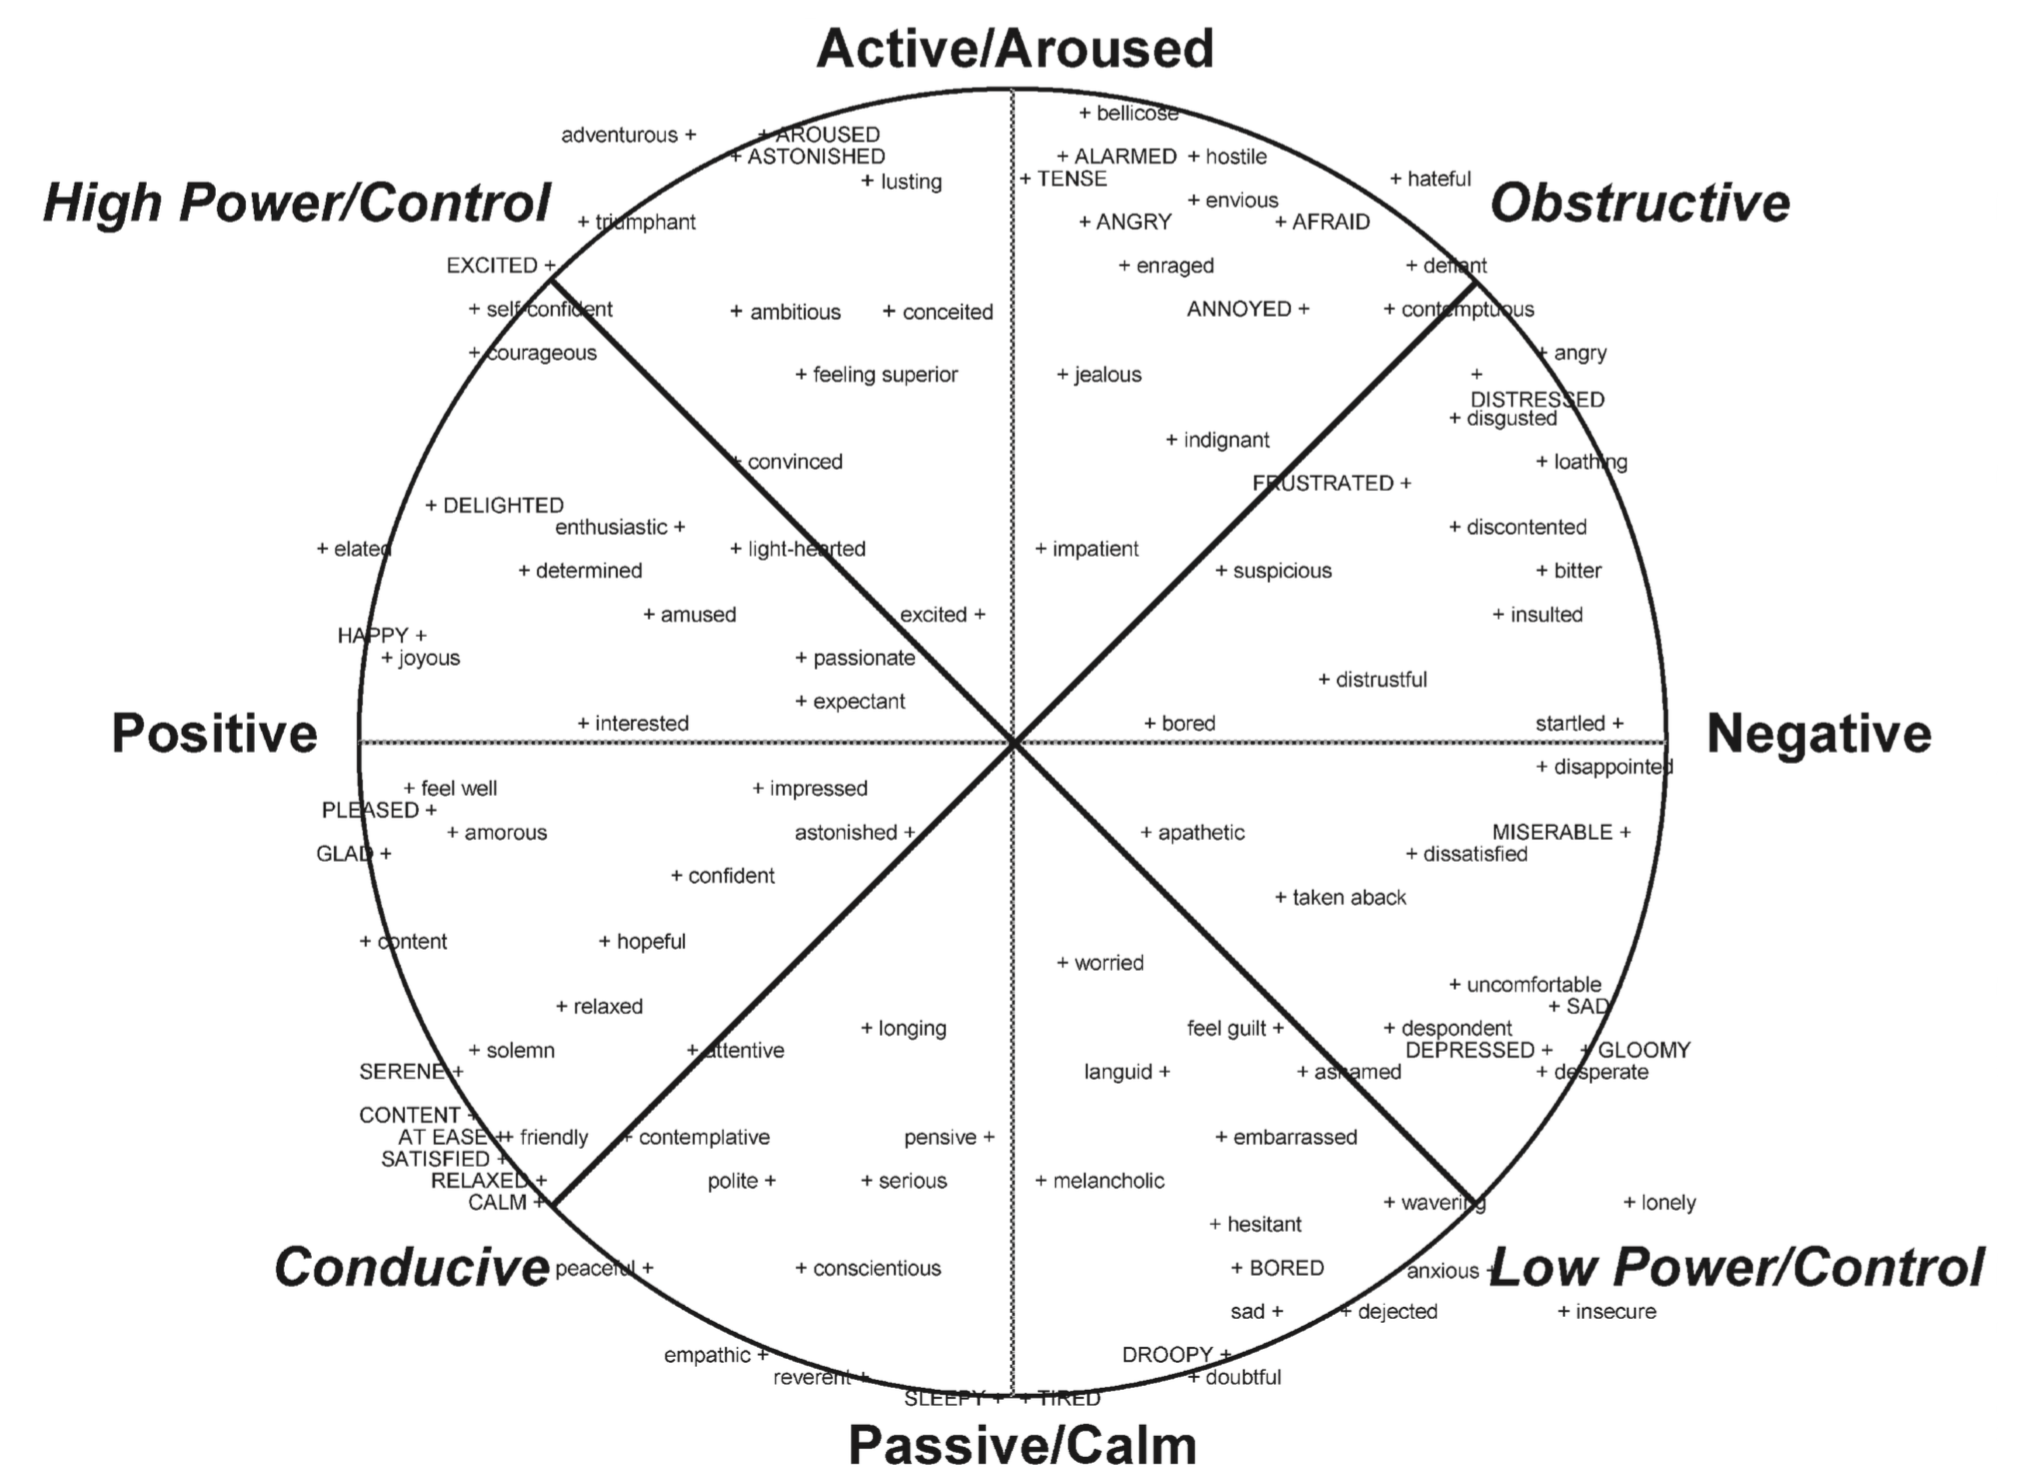
\includegraphics[width=1.0\textwidth]{EmotionSpace}
\caption{Russell's two dimensional map of emotion space}
\label{fig:emotionSpace}
\end{figure}

In order to construct the emotion - crowd type mapping, a comprehensive understanding of the behaviour of each crowd type is needed. The description of the each crowd type by \citet{Berlonghi1995} is analysed together with the definition of similar crowd types defined by other scholars. The behaviour language and trait language from those descriptions are extracted and referenced to the four emotions: fear, anger, happiness, sadness. The objective of this process is to identify the dominant emotions in each crowd type. 

\begin{itemize}
\item \textbf{Ambulatory crowd} - is characterised by the action walking and the calmness \citep{Zeitz2009}. According to \citet{russell1980circumplex}'s emotion space, \textit{calm} is located in a completely opposite region with \textit{angry} and \textit{afraid}. Although both \textit{calm} and \textit{sad} have negative level of arousal, the former has a positive degree of pleasure while the latter does not. Therefore, all four emotions are dominating in this crowd type.
\item \textbf{Disablity/Limited movement crowd} - is described by the immobility of the crowd. Similarly to the ambulatory crowd, this characteristic does not suggest any significant emotion. Hence, no emotion in the four is considered to be the dominant emotion in this crowd type.
\item \textbf{Cohesive/Spectator} - is described by the activity watching a specific event and the fact that people have the interest in watching the event. Similarly, they do not signal the dominant occurrence of any emotion.
\item \textbf{Expressive/Revellous crowd} - is characterised by the emotional release. The word \textit{revellous} originates from ``revel'' which means lively and noisy enjoyment. This indicates a high level of arousal with a positive pleasure in the \citet{russell1980circumplex}'s emotion space, which is close to \textit{happy}. Therefore, it can be inferred that this crowd type has a high intensity of \textit{happiness} as the dominant emotion.
\item \textbf{Participatory crowd} - is described by the action participating in a specific event. Although, the description does not suggest any clue on the emotional state of the participants, one example for a participatory crowd is people taking part in an actual sport event. Regarding sport psychology, studies show that sensation seeking and arousal seeking motivate the participations in sports, especially risk involved sports \citep{rowland1986sensation}. This indicates a positive level of arousal that can be observed from a participatory crowd, thus suggesting \textit{happiness} as the dominating emotion as well. Compared to expressive crowd, the intensity of \textit{happiness} can be lower.
\item \textbf{Aggressive/Hostile crowd} - is described by the verbal aggressiveness and disregard for instruction. \textit{Aggressiveness} is aroused by \textit{anger}. The \textit{aggressiveness} is limited by verbal expression, which hints that the intensity of \textit{anger} is at medium level.
\item \textbf{Demonstrator} - includes such actions as picketing, marching, protesting. According to Lofland's typology of spontaneous collective behaviours \citep{Kornblum2011}, such crowds are classified into \textit{hostile} crowd aroused by \textit{anger}. This crowd type is described to have some degree of organisation and leadership, which suggests the level of \textit{aggressiveness} is not intensive. Therefore, a low level of \textit{anger} can be considered to be the dominant emotion in this crowd type.
\item \textbf{Escaping/Trampling crowd} - is described by the escaping action from a danger or a threat. This \textit{escaping} behaviour is triggered by \textit{fear} according to Plutchik's evolutionary theory. Loftland's typology also classifies such crowd under the fearful crowd \cite{Kornblum2011}. Hence, the dominating emotion can be identified in this crowd type is clearly a high intensity of \textit{fear}.
\item \textbf{Dense/Suffocating crowd} - is characterised by the extremely high density and inability of movement in the crowd. Recent research on brain claims that suffocation might cause fear as the experiments with mice shows that inhaled carbon dioxide reduces brain pH and evokes fear behaviour \citep{ziemann2009amygdala}.
\item \textbf{Rushing/Looting crowd} - is described by the desire to acquire something. Studying the looting behaviour in London riot in 2011, \citet{ray2014shame} suggests the shame theory of violence which might has relevance in accounting for the violent disturbance. \textit{Shame} falls into the region with low arousal and negative pleasure together with the basic emotion \textit{sad}, which indicates the closeness of the two affective words. On the other hand, \textit{violence} is aroused by \textit{anger}, hence a mixture of \textit{anger} and \textit{sadness} can be considered the dominating emotions in a looting crowd.
\item \textbf{Violent crowd} - is described by the attacking, terrorising and rioting action with the complete disregard for laws and other people. Attacking is a typical behaviour triggered by \textit{anger}. This crowd type has a high level of \textit{anger}.
\end{itemize}

As we can notice from above analysis, five distinct groups of crowd types can be identified by the similarity in the dominating emotions. 
\begin{inparaenum}[i)]
\item The first group consists of ambulatory, disability/limited movement and cohesive/spectator crowd, which suggest no dominant emotion. From the emergency management point of view, those three types do not pose potential danger. Therefore, in our crowd monitoring framework, the three crowd types will be grouped and monitored as a same type.
\item The second group is characterised by \textit{happiness}. Expressive/revellous and participatory crowd belong to this group.
\item The third group is aroused by \textit{anger} and includes aggressive/hostile, demonstrator and violent crowd.
\item The fourth group is motivated by \textit{fear} consisting of escaping/trampling and dense/suffocating crowd.
\item The fifth group is rushing/looting crowd which has both \textit{anger} and \textit{sadness} as the dominant emotions.
\end{inparaenum}

\begin{table}
\caption{Mapping between crowd types and emotions}
\label{table:mappingEmotionCrowdType}
\begin{tabular}{|p{6cm}|p{1.8cm}|p{1.8cm}|p{1.8cm}|p{1.8cm}|}
\hline
\textbf{Crowd type} & \textbf{Anger} & \textbf{Fear} & \textbf{Happiness} & \textbf{Sadness} \\
\hline
Ambulatory & & & & \\
\hline
Disability / Limited movement & & & & \\
\hline
Cohesive / Spectator & & & & \\
\hline
Expressive / Revellous & & & high & \\
\hline
Participatory & & & medium & \\
\hline
Aggressive / Hostile & medium & & & \\
\hline
Demonstrator & low &  &  & \\
\hline
Violent & high & & & \\
\hline
Escaping / Trampling & & high & & \\
\hline
Dense / Suffocating	& & low & & \\
\hline
Rushing	/ Looting & medium & & & medium\\
\hline
\end{tabular}
\end{table}

\section{Rule Based Reasoning}

\subsection{Fuzzifier}
As introduced in the previous section, the emotions in the crowd are measured by the degrees of membership \(d(e_i)\) in the form of of numerical values between 0 and 1. In our mapping above, we use linguistic labels such as low, medium and high to describe the intensify of each emotion. Fuzzifier is the component converting the discrete numerical values into categorical values used in fuzzy logic. 

Firstly, the meaning of linguistic labels must be defined. Low, medium and high represent the three levels of intensity of an emotion. The intensity increase with the higher of the level. Secondly, there are certain points in the degree of membership that the intensity of an emotion changes from low level to medium level and from medium level to high level. These two points are defined as threshold \(th_1\) and \(th_2\) respectively. The conversion from crisp values of the degree of membership to linguistic label can be performed by following rules.
\[
d(e_i) \leq th_1(e_i) \Rightarrow label = low
\]
\[
d(e_i) > th_1(e_i) \land d(e_i) < th_2(e_i) \Rightarrow label = medium
\]
\[
d(e_i) \geq th_2(e_i) \Rightarrow label = high
\]
The thresholds are important to detect the abnormal increasing in one particular emotion. Firstly, because of the fact that people post unequal number of tweets in each emotion as their normal behaviour, the thresholds can be not the same for different emotions. Secondly, because of the cultural difference, the content shared on Twitter is very different across different countries and cultures. People in one country might normally post more happy content than people living in a problematic region. Moreover, even among the group of users, emotional content can also vary during different period. For example, people tend to tweet more happy content than usual around Christmas and New Year holiday. Therefore, the choice of the two thresholds for one emotion, such as happy, actually depend on the region and time. In our experiment, we propose an approach to calculate the thresholds for our experimental dataset that is collected in one specific event in the past.

\subsection{Rule Repository}

list 11 rules here for 11 crowd types

\subsection{Inference Engine}

Fuzzy rule here and the mathematical formula here

\section{Conclusion}
% !TEX root = ../thesis.tex
\chapter{Implementation and Evaluation}
\label{ch:eval}
% **************************** Define Graphics Path **************************
\ifpdf
    \graphicspath{{Chapter5/Figs/Raster/}{Chapter5/Figs/PDF/}{Chapter5/Figs/}}
\else
    \graphicspath{{Chapter5/Figs/Vector/}{Chapter5/Figs/}}
\fi

\section{Introduction}
Chapter \ref{ch:approach} has proposed a real-time Crowd Monitoring Framework based on the Emotion Analysis of Social Media. This chapter describes our strategy to implement and evaluate the proposed framework using a case study. The case study analysed a past sporting event in which a stampede occurred and caused a number of injuries in the crowd. An experimental implementation of the framework was developed involving the data collection and the emotion extraction. Our evaluation was conducted by applying a series of statistical analyses on the emotion labelled dataset.

This chapter is structured as follows. Firstly, the case study is introduced. The next sections describe our implementation of the experiment, following by the evaluation. The chapter ends with the conclusion which will give a summarised view on the evaluation of our proposed framework.

\section{A Case Study using Historical Data}

The accuracy of the crowd type classification in our proposed framework relies on the Emotion Analysis and the Rule Based Reasoning. As presented in the Chapter \ref{ch:approach}, the Emotion Analysis extracts the emotion from the collected tweets about a gathering event and computes the emotion rates in the crowd. From the emotion rate, the level of an emotion can be determined using a threshold which will be discussed in this Chapter. Based on the levels of the four emotions, the Rule Based Reasoning finally identifies the correct crowd type or the group of crowd types using a set of defined rules.

In order to evaluate the accuracy of the approach, we conducted a case study using historical data because of the following reasons. Firstly, despite the large number of mass gathering events around the world, crowd accidents do not occur very often. For this reason, a case study with real-time data might require a considerably large number of experiments with incoming events until a potential detection is found. Nevertheless, when an accidents occurs, it is difficult to identify the exact crowd types that are present in an incident without an elaborate investigation.

Using historical data enables us to select an event in the past, where a crowd related accident eventually occurred and a known crowd type was identified. Our experiment will concentrate on the data retrieval and the comparison between the identified crowd types and the analysis results using our proposed Emotion - Crowd type Mapping Model and Rule Based Reasoning. Secondly, as our Bag-of-Words were constructed from an English corpus, experimenting with historical data also enables us to focus on the events in a English speaking country where a sufficient number of tweets in English can be collected for the Emotion Analysis.

One of the disadvantages of using historical data is that the performance of the framework regarding the real-time aspect cannot be tested. In order to evaluate whether the data collection technique can gather sufficient context data to support a real-time analysis or whether the result of the analysis is produced timely enough, further researches need to be done.

\subsection{Mayweather - Maidana Post Fight Stampede}

The first step of the experiment is to select a suitable mass gathering event that matches the criteria:
\begin{inparaenum}[i)]
\item the mass gathering took place in an English speaking country;
\item a crowd accident occurred and a known crowd type was identified;
\item the event was a recent event that preferably happened after 2012
\end{inparaenum}. The reason for the last criteria is that Twitter was created in 2006 and its traffic only started booming since 2012 \footnote{http://www.internetlivestats.com/twitter-statistics/}. Therefore, it is not possible to gather tweets about an event that happened too far in the past. For these reasons, we primarily looked for recent sporting events as these events tend to involve a large number of participants in highly arousing emotions. The boxing match in USA between Floyd Mayweather and Marcos Maidana on 3th May 2014 was selected. A stampede occurred after the fight \footnote{http://www.latimes.com/sports/sportsnow/la-sp-sn-mayweather-stampede-20140504-story.html}. 

The boxing match was held at the Grand Garden Arena of the MGM Grand Hotel in Las Vegas, USA with more than 16000 people attended \footnote{http://www.usatoday.com/story/sports/boxing/2014/05/04/floyd-mayweather-marcos-maidana-stampede/8700763/}. The match started at 6:00PM local time (UTC-7). The stampede occurred around 10:45PM during the post-fight news conference. The police received an emergency call at 10:45PM reporting a gunshot at the venue \footnote{http://lasvegassun.com/blogs/kats-report/2014/may/04/dozens-injuries-reported-after-stampede-mgm-grand-/}. According to the official statement, when the fans were leaving the arena, the stampede was triggered by a loud bang of a temporary wall falling over that was mistaken as a sound of a gunshot. It caused a massive panic and people started rushing to the exits. More than 50 people were trampled and crushed in the stampede and suffered from minor injuries. The situation got under control by 1:00 AM the next day. The layout of the arena was later criticized for having only two exits and the pathway was too narrow which has caused a bottleneck \footnote{http://sports.yahoo.com/news/bob-arum--stampede-after-mayweather-maidana-was--an-accident-ready-to-happen-004057893-boxing.html}.

This event appears to satisfy the criteria for our experiment. The next section will introduce our evaluation strategy using this case study.

\subsection{Evaluation Strategy}

As a stampede was confirmed to have occurred, the known crowd types for this event can be identified as escaping and dense/suffocating which belong to Group 4 motivated by fear in our classification in Chapter \ref{ch:approach}. The objective of the experiment was to verify whether our proposed approach can identify the correct crowd types or not.

A simple implementation of the crowd monitoring framework was performed. Firstly, the tweets regarding the event to construct our experimental dataset. Secondly, the Emotion Analysis was performed to extract the emotions from the tweets using the Bag-Of-Words approach and NRC Hashtag Emotion Lexicon \citep{mohammad2014using}. Because in the real-time monitoring, tweets are collected in real time and they were analysed periodically every \(t\), the experiment was performed in a manner that can simulate the real-time analysis. The dataset was divided into smaller segments \(t_i\) and the emotion distribution in each \(t_i\) was calculated. In our implementation, interval \(t\) for a segment was set as 15 minutes.

The third step was to determine the thresholds and to label the level of an emotion in each interval. As mentioned in Chapter \ref{ch:approach}, the value of thresholds are different for each emotion and application-specific. Because of the fact that the rates of \textit{anger}, \textit{fear}, \textit{happiness} and \textit{sadness} over time were normally distributed in our dataset, a method to calculate the thresholds was implemented with moving average and z-score for each segment \(t_i\). 

Finally, the Rule Based Reasoning was implemented with the defined set of rules. The crowd types or crowd groups that possibly occurred in each \(t_i\) were inferred from the levels of the four emotions. The output of the analysis was compared with the known crowd types that were the escaping and dense/suffocating type. In term of timeliness, our detection was evaluated against the time that the accident was reported to police according to official announcement.

\section{Implementation}

\subsection{Data Collection}
There are several methods to access Twitter's data. The most common way is to access via Twitter's official Search API \footnote{https://dev.twitter.com/rest/public/search}. However, according to the documentation, the API is limited to return only tweets from the past week, hence it is not usable to retrieve historical data in our experiment. Another method is access the data from the 3rd party providers, such as Topsy \footnote{http://topsy.com} which allows to search for tweets back in the past using keywords. This website is also capable to refine the search results by date and language, yet it does not support filtering by geo-location or places. 

Our data collection requires to gather tweets related to a relatively short event. Unlike searching tweets about a celebrity or a long-term event, it is very difficult to provide the exact keywords to locate the tweets about such short term event. As we know the venue of the event, it is easier to filter for tweets by location information. Therefore, a more flexible method employing the Twitter Advanced Search \footnote{https://twitter.com/search-advanced} and web crawling technique was introduced in our experiment.

\subsubsection{Twitter Advanced Search}
Twitter Advanced Search is in fact a built-in functionality on Twitter's homepage, which allows to search for any tweet on Twitter. It supports searching with keywords, date range, places and most importantly, it does not have any restriction in term of historical data \footnote{https://support.twitter.com/articles/71577-using-advanced-search}. This functionality is also freely accessible through the Twitter website without any authentication.

On the other hand, since the Advanced Search is designed for the user who accesses Twitter via a browser, the search result is displayed in a web page in HTML format. It does not support exporting the data to any format that is programmatically readable. Another technical challenge is that the search results are wrapped inside a scrolling pane, which requires the scrolling action from the user to fetch more data. 

In conclusion, although Twitter Advanced Search is very a potential source to collect historical tweets, it is not designed to be programmatically accessed. However, because our experiment required a larger number of tweets to perform analysis, it was impractical to manually perform the data collection. Therefore, the web crawling technique was incorporated to automate the process.

\subsubsection{Crawling the Twitter Advanced Search}
In order to programmatically access Twitter Advanced Search, PhantomJS and CasperJS were utilized in our data collection process. PhantomJS \footnote{http://phantomjs.org} is headless scripted browser which is used to automate web page interaction for testing purposes. CasperJS \footnote{http://casperjs.org} is an open source JavaScript tool written for PhantomJS to enhance various tasks including the DOM manipulation. The complete crawling process consisting of visiting Twitter page, submitting the search queries, scrolling down the result list and parsing the data from the DOM were written in JavaScript as step by step instructions for the headless browser to operate accordingly. As a result, the headless browser could imitate the human interaction on a normal browser to search for tweets and automatically store the parsed data into Comma-separated Values (CSV) files. The detail of the software used for the implementation of the crawler is listed in Table \ref{table:crawlerSoftware}.

\begin{table}[!h]
\caption{Software used to crawl Twitter Advanced Search}
\label{table:crawlerSoftware}
\centering
\begin{tabular}{|l|l|l|l|}

\hline
\textbf{Software} & \textbf{Version} & \textbf{License} & \textbf{Language} \\ \hline \hline
PhantomJS & 1.98 & BSD & JavaScript \\ \hline
CasperJS & 1.1-beta3 & MIT & JavaScript \\ \hline

\end{tabular}
\end{table}

On the website, Twitter Advanced Search offers a form to input the search criteria. After submitting the form, it generates an HTTP GET to perform the search action. The parameters of the HTTP GET are described in Table \ref{table:crawlerRequest}. These parameters helped to construct the HTTP GET request used by our crawler.

\begin{table}[!h]
\caption{Twitter Advanced Search Request}
\label{table:crawlerRequest}
\centering
\begin{tabular}{|p{2cm}|p{10cm}|}

\hline
\textbf{Parameter} & \textbf{Description} \\ \hline \hline
f & Sorting order of the returned tweets. \textit{realtime} sorts the tweets by posted date while \textit{top} sorts the most popular tweets first \\ \hline
q & The query string for each search \\ \hline
src & Source of the action, normally set as \textit{typd} \\ \hline
\end{tabular}
\end{table}

The query string was the most important parameter of the search. Although, the event only lasted for a few hours, in order to investigate the distribution of emotions during the time around the event, a longer sampling period was desirable. The two parameters of the query string \textit{since} and \text{until} were set as \textit{2014-05-01} and \textit{2014-05-07} respectively to collect seven days of tweets. Because our analysis only supports English, the parameter \textit{lang} was set as \textit{eng} to filter out tweets written in other languages. Because the selected event were rather short, it did not have a dedicated hashtag like \#australianopen for the Australian Open tennis tournament. Our data collected relied on the venue of the event to search for tweets. As the venue of the boxing match was MGM Grand Hotel, the parameter \textit{near} was set to the coordinates of the hotel \footnote{36.102552, -115.169569} and \textit{within} parameter was set to 3 miles. The search engine returned all tweets that were either geotagged or checked in with a place that lied within the radius of specified area. It was also noticeable in the returned tweets that there were a large number of tweets containing the mention \textit{@MGMGrand} or the hashtag \textit{\#MGMGrand}. They suggested to be a possible keyword for an alternate search for tweets at the venue. Therefore, we ran another crawler with similar parameters but searching for keyword \textit{MGMGrand} instead of specifying the location. The query string used by two crawlers are presented in Table \ref{table:crawlerURL}. The implementation of the crawler using CasperJS is shown in Listing \ref{lst:crawler}. 

\begin{table}[!h]
\caption{Twitter Advanced Query String}
\label{table:crawlerURL}
\centering
\begin{tabular}{|p{3.5cm}|p{11cm}|}

\hline
\textbf{Search target} & \textbf{Query string} \\ \hline \hline
Venue's coordinates & q=lang:en near:"36.102552, -115.169569" within:3mi since:2014-05-01 until:2014-05-07 \\ \hline
Hashtag \& mention & q=MGMGrand lang:en since:2014-05-01 until:2014-05-07 \\ \hline

\end{tabular}
\end{table}

\clearpage
\begin{lstlisting}[language=JavaScript,caption=Crawling Twitter Advanced Search with CasperJS,label=lst:crawler]
var fs = require('fs');
var system = require('system');
var casper = require('casper').create();

var query = 'lang:en near:"36.102552, -115.169569" within:3mi since:2014-05-01 until:2014-05-07';
var search_api = 'https://twitter.com/search?f=realtime&q=' + encodeURIComponent(query) + '&src=typd';
casper.thenOpen(search_api, function(){
	scroll(this);
});

casper.then(function(){
	fs.write('result.csv', '', 'w');
	var nodes = this.evaluate(function(){
		var items = document.querySelectorAll('li.stream-item');
		return Array.prototype.map.call(items, function(e) {
			// parsing HTML to get data
			var id = e.getAttribute('data-item-id');
			
			var tag_username = e.querySelector('span.username b');
			var username = tag_username ? tag_username.innerHTML : '';
			
			var tag_timestamp = e.querySelector('small.time a.tweet-timestamp span'); 
			var timestamp = tag_timestamp ? tag_timestamp.getAttribute('data-time-ms') : '';
			
			var tag_text = e.querySelector('div.content p.tweet-text');
			var text = tag_text ? tag_text.innerHTML : '';
			return {'id' : id, 'username' : username, 'timestamp' : timestamp, 'text' : text};
		});		
	});
	this.echo('number of tweets: ' + nodes.length);
	for(var i = 0; i < nodes.length; i ++){
		var node = nodes[i];
		// write to CSV file
		fs.write("result.csv", '"' + node['id'] + '"\t"' + node['username'] + '"\t"' + node['timestamp'] + '"\t"' + node['text'] + '"\r\n', 'a');	
	}		
})

function scroll(_casper){
	_casper.waitFor(
		function scrollBottom(){
			// try scrolling page down by 500px
			this.page.scrollPosition = {top: this.page.scrollPosition["top"] + 500, left: 0};
			this.wait(100);
			return true;
		}, function then(){
			// error loading
			if(this.exists('div.has-items-error')){
				// click on retry button
				this.click('a.try-again-after-whale');
				this.then(function() {
					return scroll(_casper);
				});
			}
			// more item below 
			else if(this.exists('div.has-more-items')){
				return scroll(_casper);
			}
			// end scrolling
		}, function onTimeout(){
		}, 10000);
}
casper.run();
\end{lstlisting}

Finally, a dataset containing 33935 tweets over 7 days was collected and it was used as our experimental dataset to evaluate our Emotion Analysis and Rule Based Reasoning.

\subsection{Emotion Analysis}
As mentioned in Chapter \ref{ch:approach}, our Emotion Analysis is based on a Bag-of-Words approach. For our experiment, a simple Java application was implemented to perform the Emotion Analysis. The Java application employed the Stanford Tokenizer \footnote{http://nlp.stanford.edu/software/tokenizer.shtml} to break a tweet into words and the NRC Hashtag Emotion Lexicon \citep{mohammad2014using} as baseline for the association scoring.

\subsubsection{Stanford Tokenizer}
The Stanford Tokenizer is a English tokenizer developed by Stanford NLP Group \citep{manning-EtAl:2014:P14-5}, which can divide text into a sequence of tokens or words. In term of efficiency, the Stanford Tokenizer can tokenize text at the rate of 200000 tokens per second. It is distributed as a part of Stanford CoreNLP \footnote{http://nlp.stanford.edu/software/corenlp.shtml} library in Java licensed under GNU General Public License (GPL). Our Java application ran the tokenizer via the APIs offered in PTBTokenizer class.

\subsubsection{NRC Hashtag Emotion Lexicon}
The NRC Hashtag Emotion Lexicon is a part of the NRC Hashtag Emotion Corpus by \citet{mohammad2014using}, which collected tweets with emotion-word hashtags. The lexicon is a list of words and their associations with \citep{plutchik2001nature}'s eight emotions: \textit{anger}, \textit{fear}, \textit{anticipation}, \textit{trust}, \textit{surprise}, \textit{sadness}, \textit{joy} and \textit{disgust}. The association called SoA, was calculated from the frequency of a word appearing in the tweets tagged with an emotion as can be seen in Formula \ref{eq:soA}.

\begin{equation}
\label{eq:soA}
	SoA(w, e) = PMI(w, e) - PMI(w, \neg{e})
\end{equation}
where PMI is pointwise mutual information, calculated by Formula \ref{eq:pmi} and \ref{eq:pmiNegate}
\begin{equation}
\label{eq:pmi}
	PMI(w, e) = log_2\frac{freq(w, e) * N}{freq(w) * freq(e)}
\end{equation}
\begin{equation}
\label{eq:pmiNegate}
	PMI(w, \neg{e}) = log_2\frac{freq(w, \neg{e}) * N}{freq(w) * freq(\neg{e})}	
\end{equation}
where \(freq(w,e)\) is the number of times word \(w\) occurs in a tweet labelled with \(e\). \(freq(w)\) and \(freq(e)\) are the frequencies of \(w\) and \(e\) in the NRC Hashtag Emotion Corpus.

Our Java based implementation used version 0.2 of the NRC Hashtag Emotion Lexicon released in November 2013 with 16862 words \footnote{http://www.saifmohammad.com/WebPages/lexicons.html}. The lexicon was distributed in a Tab-separated Values (TSV) file. The file was read into our Java application during bootstrap and stored in memory. Since our approach employed the simplified emotion model with four basic emotions: \textit{anger}, \textit{fear}, \textit{happiness} and \textit{sadness}, only the SoA scores for \textit{anger}, \textit{fear}, \textit{joy} and \textit{sadness} were used in our Java application.

\subsubsection{Java Based Implementation}
The Emotion Analysis was performed by a Java application. The first phase was the bootstrap, in which the CSV file containing the collected tweets and the TSV file containing the NRC Hashtag Emotion Lexicon were read into the memory. The Lexicon was stored as a HashMap for random access with the word served as the key of each record in the HashMap. The value of each record was an Word Object which consisted of a four-element array of doubles holding the SoA of that emotion toward \textit{anger}, \textit{fear}, \textit{happiness} and \textit{sadness}. If the SoA against an emotion was not found from the Lexicon, the value was set as \(\epsilon\) which referred to a very small number \(10^{-6}\). This array was the implementation of the emotional weight vector of that particular word. The collected tweets were stored as an ArrayList for sequential access. 

The second phase was the analysis, where each tweet in the ArrayList was tokenized by PTBTokenizer into words and the weight vector of each word was retrieved from the HashMap. The summative emotional weight vector of the tweet was calculated to extract the dominant emotion and save it as an attribute in each tweet. After finishing looping through the ArrayList of tweets, the application stored all tweets into a database where each record was a tweet labelled with \textit{anger}, \textit{fear}, \textit{happiness}, \textit{sadness} or \textit{unknown}. The \textit{unknown} class was labelled to tweets which no dominant emotion was found.

The algorithm \ref{algorith:pseudocode} describes our Java implementation of the Emotion Analysis. Our database was running MySQL version 5.5.41 \footnote{https://www.mysql.com}. Collected tweets were saved in the SAMPLES table which structure is presented in Table \ref{table:databaseTweet}.

\begin{algorithm}
\begin{algorithmic}[1]
\BState \emph{ReadLexicon}:
	\State $WordMap$ $\gets$ initialize a HashMap
	\State $LexiconFile$ $\gets$ read from TSV file
	\ForAll {$Row \in LexiconFile$}
		\State $Word$ $\gets$ read word field from $Row$
		\State $Emotion$ $\gets$ read emotion field from $Row$
		\State $SoA$ $\gets$ read SoA score field from $Row$

		\If {$Word \not\in WordMap$}
			\State add $Word$ to $WordMap$
		\Else
			\State $Word$ $\gets$ get from $WordMap$
		\EndIf
		\State set $Emotion$ of $Word$ as $SoA$
	\EndFor
\BState \emph{ExtractEmotion}:
	\State $TweetList$ $\gets$ initialize an ArrayList
	\State $TweetFile$ $\gets$ read from CSV file
	\ForAll{$Row \in TweetFile$}
		\State $Message$ $\gets$ read content field from $Row$

		\State $Anger$ $\gets$ initialize as $\epsilon$
		\State $Fear$ $\gets$ initialize as $\epsilon$
		\State $Happiness$ $\gets$ initialize as $\epsilon$
		\State $Sadness$ $\gets$ initialize as $\epsilon$

		\State $Tokens$ $\gets$ tokenize $Message$
		\ForAll{$Word \in Tokens$}
			\If{$Word \in WordMap$}
				\State $Word$ $\gets$ get from $WordMap$
				\State $Anger$ $\gets$ add up SoA score of anger from $Word$
				\State $Fear$ $\gets$ add up SoA score of fear from $Word$
				\State $Happiness$ $\gets$ add up SoA score of happiness from $Word$
				\State $Sadness$ $\gets$ add up SoA score of sadness from $Word$
			\EndIf
		\EndFor
		\State $LabelledEmotion$ $\gets$ $max(Anger, Fear, Happiness, Sadness)$
		\State insert $Message$ and $LabelledEmotion$ into database
	\EndFor
\end{algorithmic}
\caption{Emotion Analysis}
\label{algorith:pseudocode}
\end{algorithm}

\begin{table}[hb!]
\centering
\caption{Database containing tweets and their labelled emotion}
\label{table:databaseTweet}
\begin{tabular}{|l|l|l|}

\hline
\textbf{Column name} & \textbf{Data type} & \textbf{Description} \\ \hline \hline
tweet\_id & BIGINT(20) & Unique ID of a tweet \\ \hline
user\_id & VARCHAR(20) & ID of the author of the tweet \\ \hline
user\_name & VARCHAR(50) & Username of the author \\ \hline
created & DATETIME & The timestamp when the tweet was posted \\ \hline
text & TEXT & The content of the tweet \\ \hline
emotion & VARCHAR(10) & The emotion labelled with the tweet \\ \hline
\end{tabular}
\end{table}

\clearpage
\subsubsection{Emotion Rate, Threshold and Level of an Emotion}
The output of the Java application was a database containing tweets and their labelled emotions. According to the evaluation plan, the next step was to simulate the real-time monitoring by dividing the dataset into 15 minute segments and then applying the statistical tests on the data in each segment. The grouping was performed in the database by running an SQL as shown in Listing \ref{lst:sqlGrouping}. This SQL grouped the tweets into each 15 minute segment and counted the number of tweets in each segment. The result consisting of 576 consecutive segments was exported to a CSV file for statistical analysis in Microsoft Excel. Each segment was saved as a row and the numbers of tweets labelled with each emotion was stored as a column.

\begin{lstlisting}[language=SQL,caption=Segment Division in SQL,label=lst:sqlGrouping]
SELECT YEAR(created), MONTH(created), DAY(created), 
HOUR(created), FLOOR(MINUTE(created) / 15) * 15 AS MINUTE, 
COUNT(tweet_id) 
FROM samples 
GROUP BY YEAR(created), MONTH(created), DAY(created), 
HOUR(created), FLOOR(MINUTE(created) / 15);
\end{lstlisting}

The Emotion Distribution in a segment was done by calculating the rate of \textit{anger}, \textit{fear}, \textit{happiness} and \textit{sadness}. As mentioned in the Chapter \ref{ch:approach}, the rate of an emotion is computed by dividing the number of tweets labelled with that emotion by the total number of tweets. Since there existed tweets labelled with \textit{unknown} emotion in our dataset, in order to keep the summative of the rates of four emotion to 1.0, the total number of tweets only counted the tweets labelled with \textit{anger}, \textit{fear}, \textit{happiness} or \textit{sadness} while ignoring the \textit{unknown} label. The result of this operation was the emotion distribution in 576 consecutive 15 minute segments. 

A study in the distribution of the rates of the four emotion across 576 segments showed that the distribution of an emotion rate followed the normal distribution. This finding was obtained by apply histogram analysis on the rates of the four emotions during the sampled period. The result of the histogram analysis will be discuss further in the Section \ref{sec:evaluation}. Based on the normal distribution of the emotion rate, a method to determine the threshold was proposed by using moving average and z-score on the emotion rate in each segment. 

Moving average is a popular technique for making short term forecasting. In this case, moving average and z-score was effective to detect the changes in the intensity of an emotion. In other words, the emotion rate of an emotion was compared relatively with the data in the latest hour to determine whether its intensity was high or not. For each segment, the moving average was calculated by getting the average value of the emotion rates in a moving window consisting of that segment and four previous segments, as shown in Formula \ref{eq:movingAvg}.

\begin{equation}
\label{eq:movingAvg}
	SMA(e_i)_{t_j} = \frac{ rate(e_i)_{t_j} + rate(e_i)_{t_{j-1}} + rate(e_i)_{t_{j-2}} + rate(e_i)_{t_{j-3}} + rate(e_i)_{t_{j-4}} }{5}
\end{equation} 

where, \(e_i\) is an emotion of the four emotions: \textit{anger}, \textit{fear}, \textit{happiness} and \textit{sadness}. \(t_j\) is a segment at interval \(j\). \(SMA(e_i)\) is the moving average of the emotion rate of \(e_i\) and \(rate(e_i)\) is the emotion rate of \(e_i\). According to the normal distribution, this average value was the expected value of the emotion rate with highest probability. To represent how far an emotion rate of \(e_i\) was lower or higher than the expected value value \(SMA(e_i)\), the z-score was employed and computed by Formula \ref{eq:zscore}.

\begin{equation}
\label{eq:zscore}
	z(e_i) = \frac{rate(e_i) - SMA(e_i)}{\sigma(e_i)}
\end{equation}
where, \(e_i\) is an emotion of the four basic emotions. \(rate(e_i)\) is the emotion rate of emotion \(e_i\), \(SMA(e_i)\) is the moving average of \(e_i\) and \(\sigma(e_i)\) is the standard deviation of the emotion rate of \(e_i\) within the moving window. 

Because z-score was a normalized value, the z-scores of the four emotions can be compared with each other. We defined \(z = 1.0\) as the global high level threshold across all emotions. If the z-score of one emotion exceeded 1.0, the level of that emotion was marked as high in that segment (Formula \ref{eq:zscoreHighLevel}).

\begin{equation}
\label{eq:zscoreHighLevel}
	z(e_i) > 1 \Rightarrow level(e_i) = high
\end{equation} 

\subsection{Rule Based Reasoning}
The Rule Based Reasoning was also implemented in Microsoft Excel as five IF statements according to the five rules defined in Chapter \ref{ch:approach}.

\section{Evaluation}
\label{sec:evaluation}
\subsection{Experimental Dataset}
Our experimental dataset contained 33935 tweets. Briefly talk about the dataset: diagram showing distribution by days. Applying the Emotion Analysis using NRC Hashtag Emotion Lexicon \citep{mohammad2014using} on the dataset, 28698 tweets were labelled with one of four emotions: \textit{anger}, \textit{fear}, \textit{happiness} and \textit{sadness}. Figure \ref{fig:emotionLabel} shows 5237 tweets that were unable to label with any emotion thus being marked as unknown. Overall, the Bag-of-Words approach successfully extracted the emotion from 84.67\% of the collected tweets. Our statistical analysis was performed on the labelled data.

\begin{figure}[!htb]
\centering
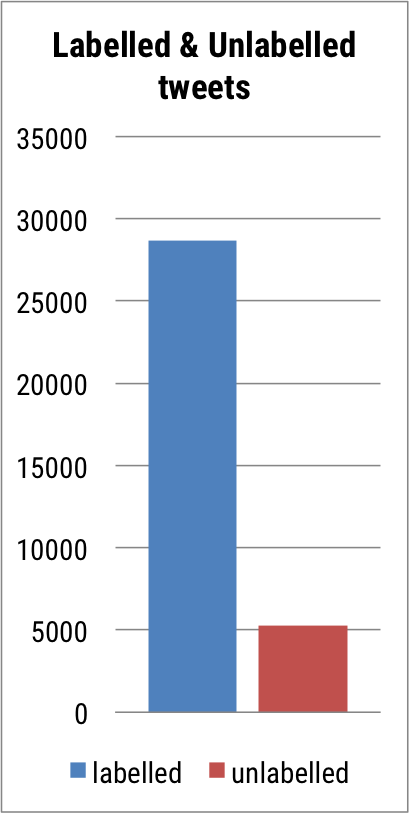
\includegraphics[width=0.3\textwidth]{EmotionLabel}
\caption{The result of emotion extraction from the dataset}
\label{fig:emotionLabel}
\end{figure}

\begin{figure}[!htb]
\centering 
\begin{subfigure}{0.5\textwidth}
\centering
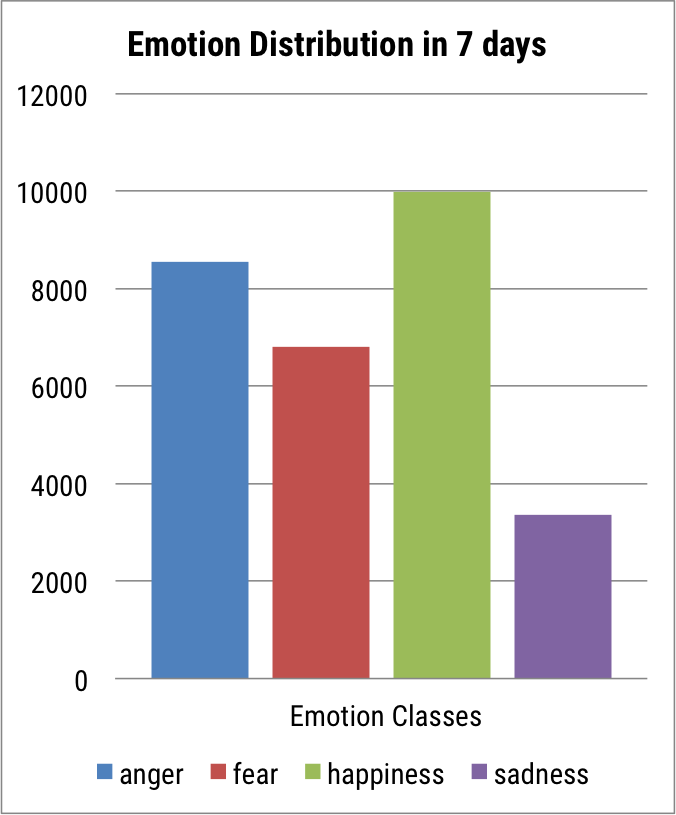
\includegraphics[width=0.75\linewidth]{EmotionDistributionWeek}
\caption{Seven days}
\label{fig:emotionDistributionWeek}
\end{subfigure}%
\begin{subfigure}{0.5\textwidth}
\centering
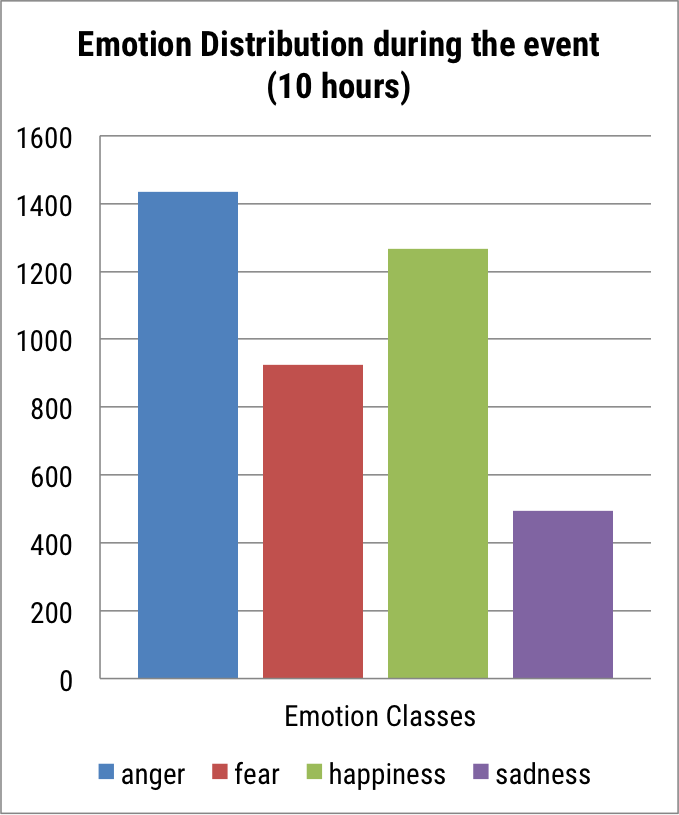
\includegraphics[width=0.75\linewidth]{EmotionDistributionEvent}
\caption{During event}
\label{fig:emotionDistributionEvent}
\end{subfigure}
\caption{The number of tweets labelled with each emotion in the whole dataset of seven days and during the event}
\end{figure}

Among the labelled tweets, the number of tweets in each emotion was not equally distributed as can be seen in Figure \ref{fig:emotionDistributionWeek}. This finding further supports the argument mentioned in Chapter \ref{ch:approach} that the users tend to post more happy content than the other emotions. 

The boxing match started at 6:00PM local time on May 3rd, while the stampede occurred around 10:45PM and the situation was reported to get under control at 1:00AM. There points were helpful to identify the time period that could be considered to be related to the event. The event was defined as a 7 hour period starting from 6:00PM to 1:00 AM. Our statistical analysis emphasised on this period. Figure \ref{fig:emotionDistributionEvent} illustrates the distribution of emotions during this event. As can be seen, the dominating emotion was \textit{anger}. The reason might be because of the nature of the boxing match that the related tweets contained lots of aggressive words.

\subsection{Statistical Analysis}

\subsubsection{Number of tweets labelled in each emotion over time}
Figure \ref{fig:emotionInstanceEvent} illustrates the change in the number of tweets labelled in each emotion over time. The horizontal axis presents our focused time-line consisting of 29 segments. The vertical axis shows the total number of tweets labelled with a specific emotion within a segment. The highlighted area between 10:45PM and 11:30PM illustrates the time when the stampede was reported to occur.

\begin{figure}[!htbp] 
\centering
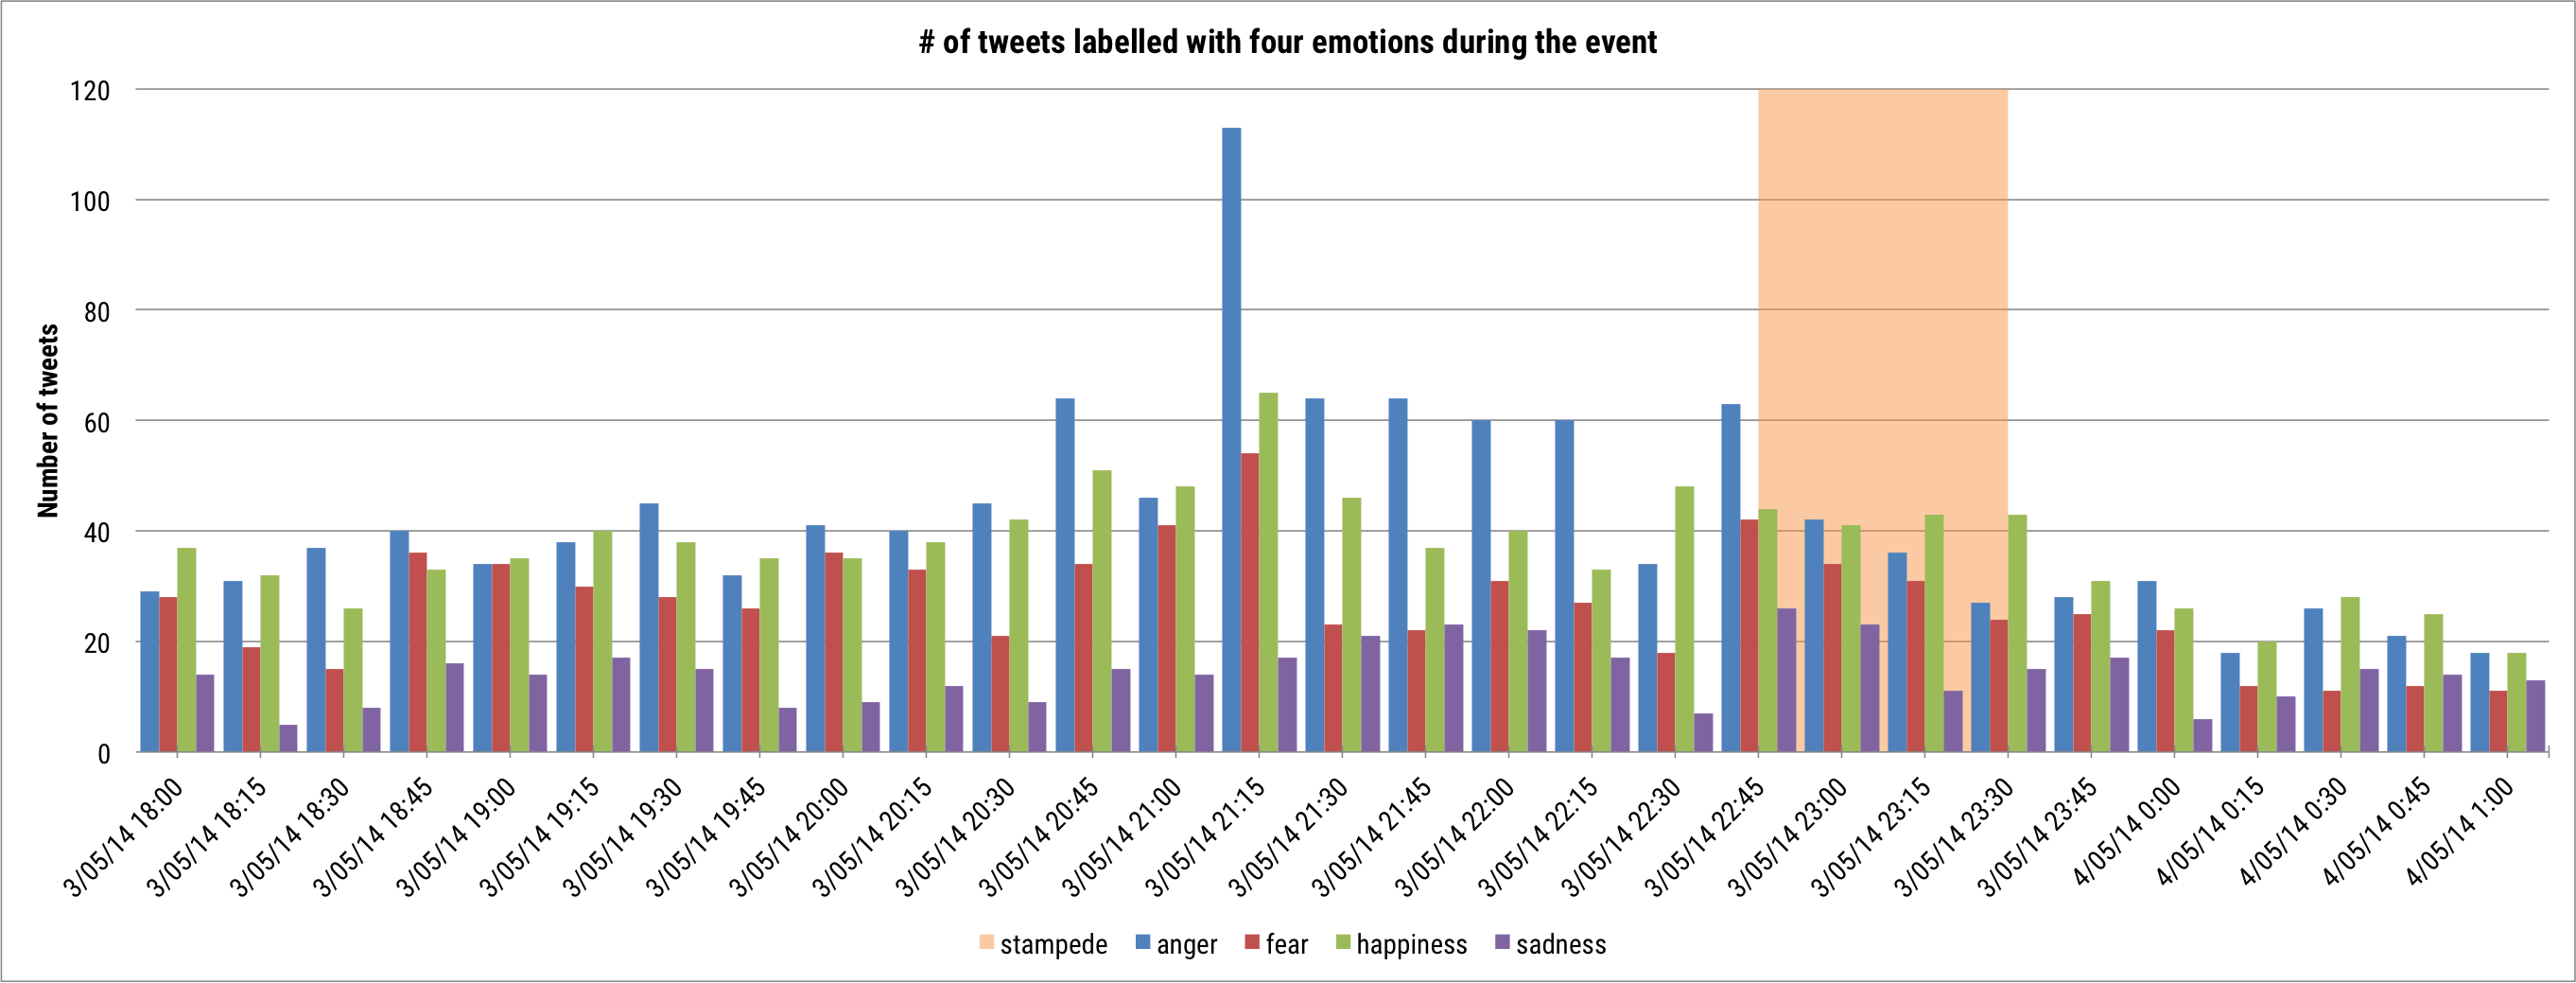
\includegraphics[width=1.0\linewidth]{EmotionInstanceEvent}
\caption{The number of tweets labelled with anger, fear, happiness and sadness during the event}
\label{fig:emotionInstanceEvent}
\end{figure}

As can be noticed from the charts, \textit{anger} labelled tweets reached a sudden peak at May 3rd 9:15PM. The number of tweets labelled with \textit{fear} and \textit{happiness} were also considerably high in this segment. Because of the overall increase trend across all emotions, the change caused by \text{anger} became less significant because there were increases in other emotions as well.

In conclusion, the number of tweets was not a robust measure to identify changes in emotion because it was affected by the overall trend. This also explained why emotion rate was selected as the measure in our approach.

\subsubsection{Emotion rate of each emotion over time}
Figure \ref{fig:emotionRateEvent} shows the emotion distribution over time using the emotion rate. 

\begin{figure}[!htbp] 
\centering
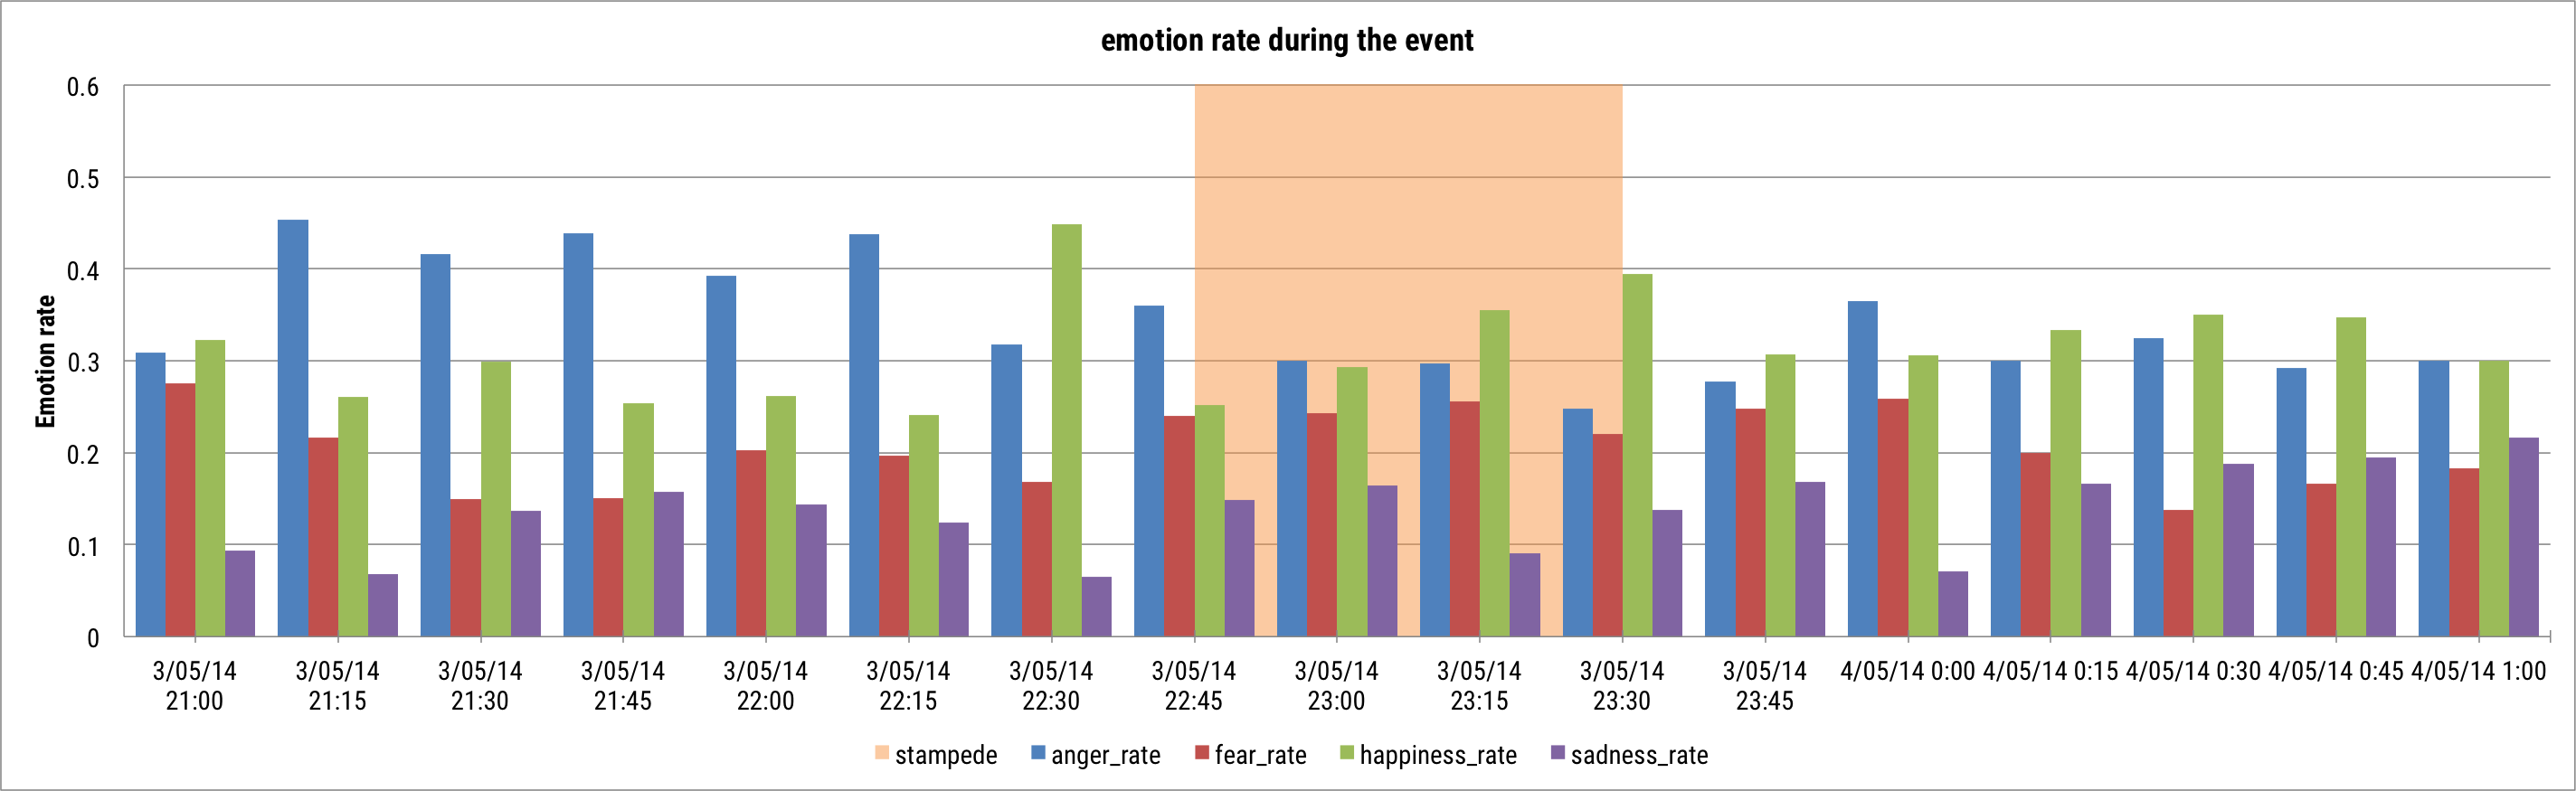
\includegraphics[width=1.0\linewidth]{EmotionRateEvent}
\caption{The percentage of anger, fear, happiness and sadness over time during the event}
\label{fig:emotionRateEvent}
\end{figure}

As can be seen, during the highlighted segments, \textit{happiness} was the emotion that had the highest rate among the four emotions. However, this rate started relatively high compared to other emotions at the beginning of the event period. Secondly, as mentioned earlier, the proportion of happiness labelled tweets was generally larger than other emotions during the seven days of sampling period. Therefore, a high value of the emotion rate can not be inferred to the behaviour of the crowd at a certain time. In fact, the changes of emotion rate over time was more important to identify abnormal behaviour in the crowd. This explained the use of moving average and z-score of emotion rate proposed in our implementation.

\subsubsection{The normal distribution of emotion rate over time}
This section investigates the distribution of emotion rate over time. By applying histogram to the emotion rate over time of each emotion, the distribution of the emotion rate followed the normal distribution. The majority of the values were close to the mean values forming a bell shape, as can be seen in Figure \ref{fig:histogramWeek}. In a normal distribution, the further a value deviates from the mean value, the less frequently it appears, thus suggesting a lower probability of occurrence. As mentioned earlier, the high level threshold was proposed as \(+1.0\). Because of the normal distribution, the probability of a high level emotion to occur is 15.8\%.

\begin{figure}[!h] 
\centering    
\begin{subfigure}{0.5\textwidth}
\centering
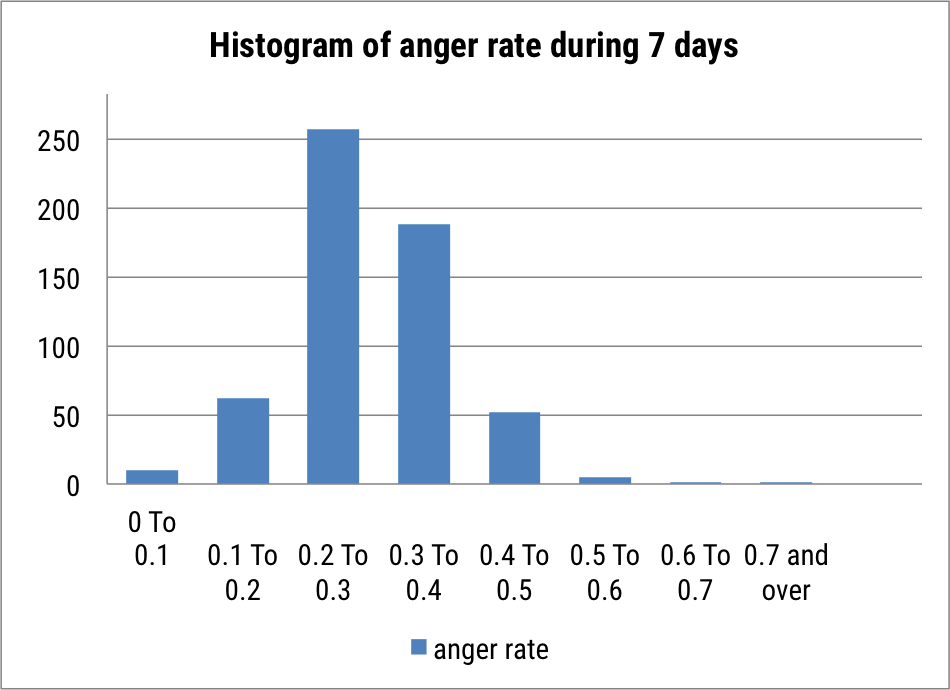
\includegraphics[width=0.98\linewidth]{HistogramAngerWeek}
\caption{anger}
\label{fig:histogramAngerWeek}
\end{subfigure}%
\begin{subfigure}{0.5\textwidth}
\centering    
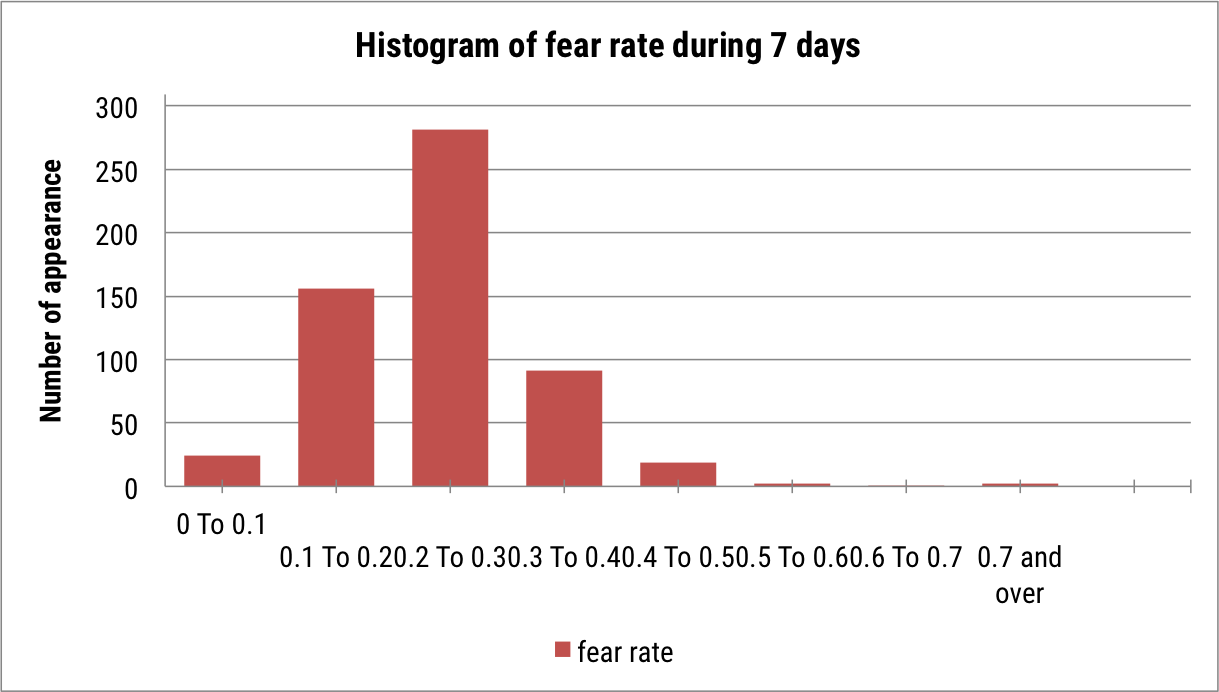
\includegraphics[width=0.98\linewidth]{HistogramFearWeek}
\caption{fear}
\label{fig:histogramFearWeek}

\end{subfigure}
\begin{subfigure}{0.5\textwidth}
\centering    
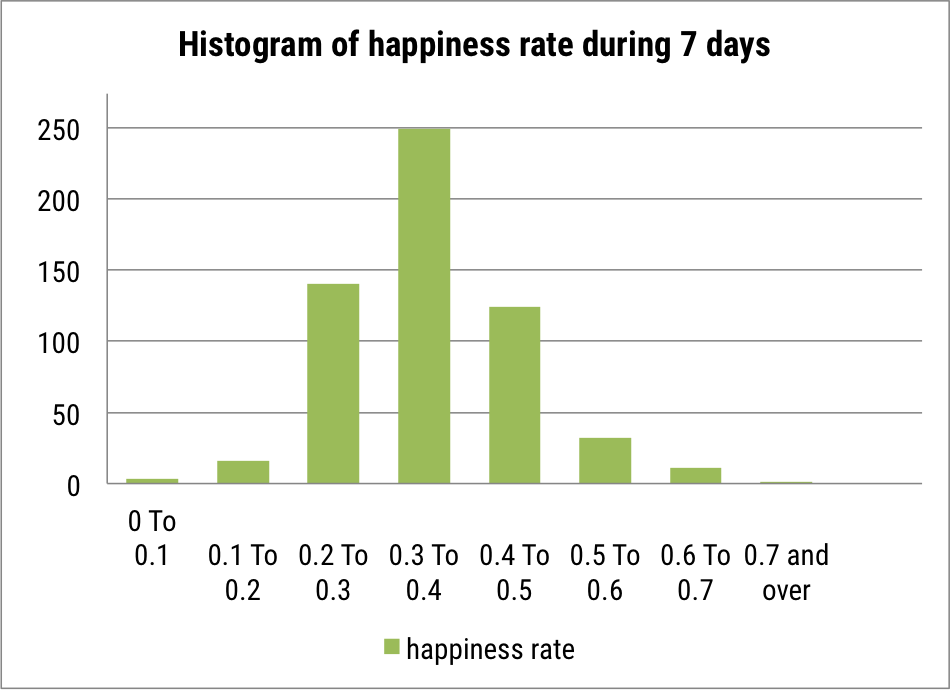
\includegraphics[width=0.98\linewidth]{HistogramHappinessWeek}
\caption{happiness}
\label{fig:histogramHappinessWeek}
\end{subfigure}%
\begin{subfigure}{0.5\textwidth}
\centering    
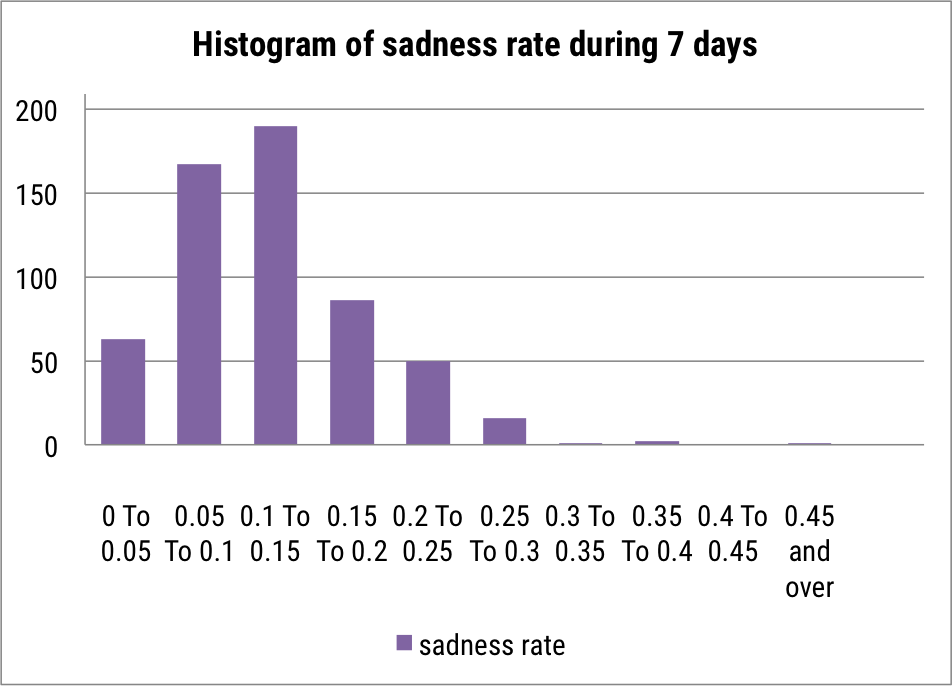
\includegraphics[width=0.98\linewidth]{HistogramSadnessWeek}
\caption{sadness}
\label{fig:histogramSadnessWeek}
\end{subfigure}
\caption{The normal distribution of anger, fear, happiness and sadness emotion rate over time in the dataset}
\label{fig:histogramWeek}
\end{figure}

\subsubsection{Z-score and the level of an emotion}
In statistics, z-score is a normalized score representing whether an observed value is lower or higher than the mean value and how far the deviation is. In our experiment, z-score was effective when combined with moving average to detect changes in emotion rate. Figure \ref{fig:emotionZscoreEvent} presents the z-score of emotion rate of the four emotions over time during the event. As can be seen, at 10:45PM when the stampede was reported to start, the z-scores of \textit{anger} and \textit{happiness} emotion rate were negative, suggesting that their emotion rates were below the expected value. On the other hand, the z-scores of \textit{fear} and \textit{sadness} emotion rate were positive. 

\begin{figure}[!htb] 
\centering
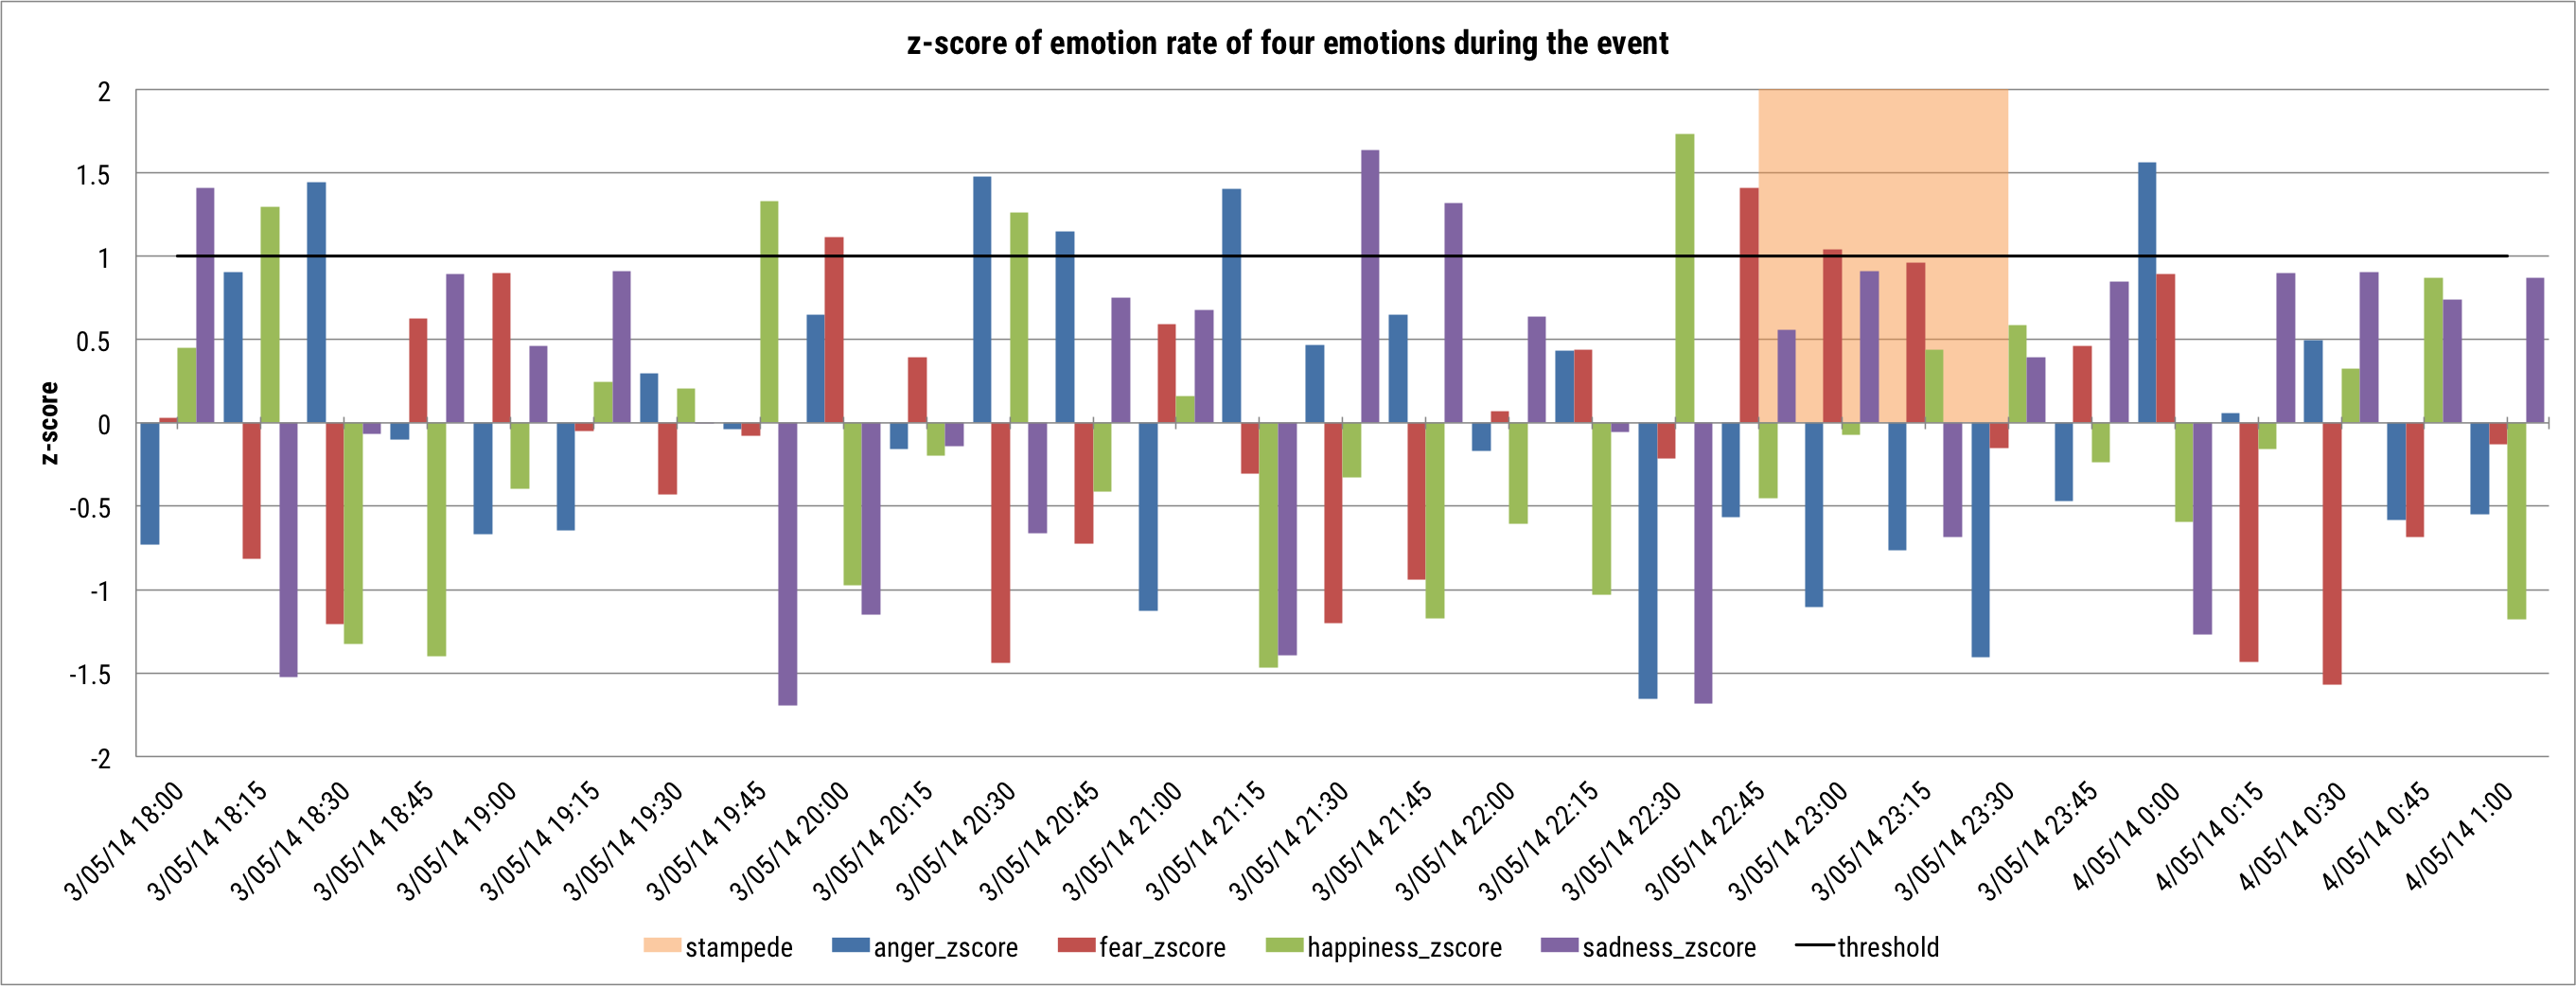
\includegraphics[width=1.0\linewidth]{EmotionZscoreEvent}
\caption{The z-score of anger, fear, happiness and sadness rate over time during the event}
\label{fig:emotionZscoreEvent}
\end{figure}

\begin{figure}[!htb]
\centering
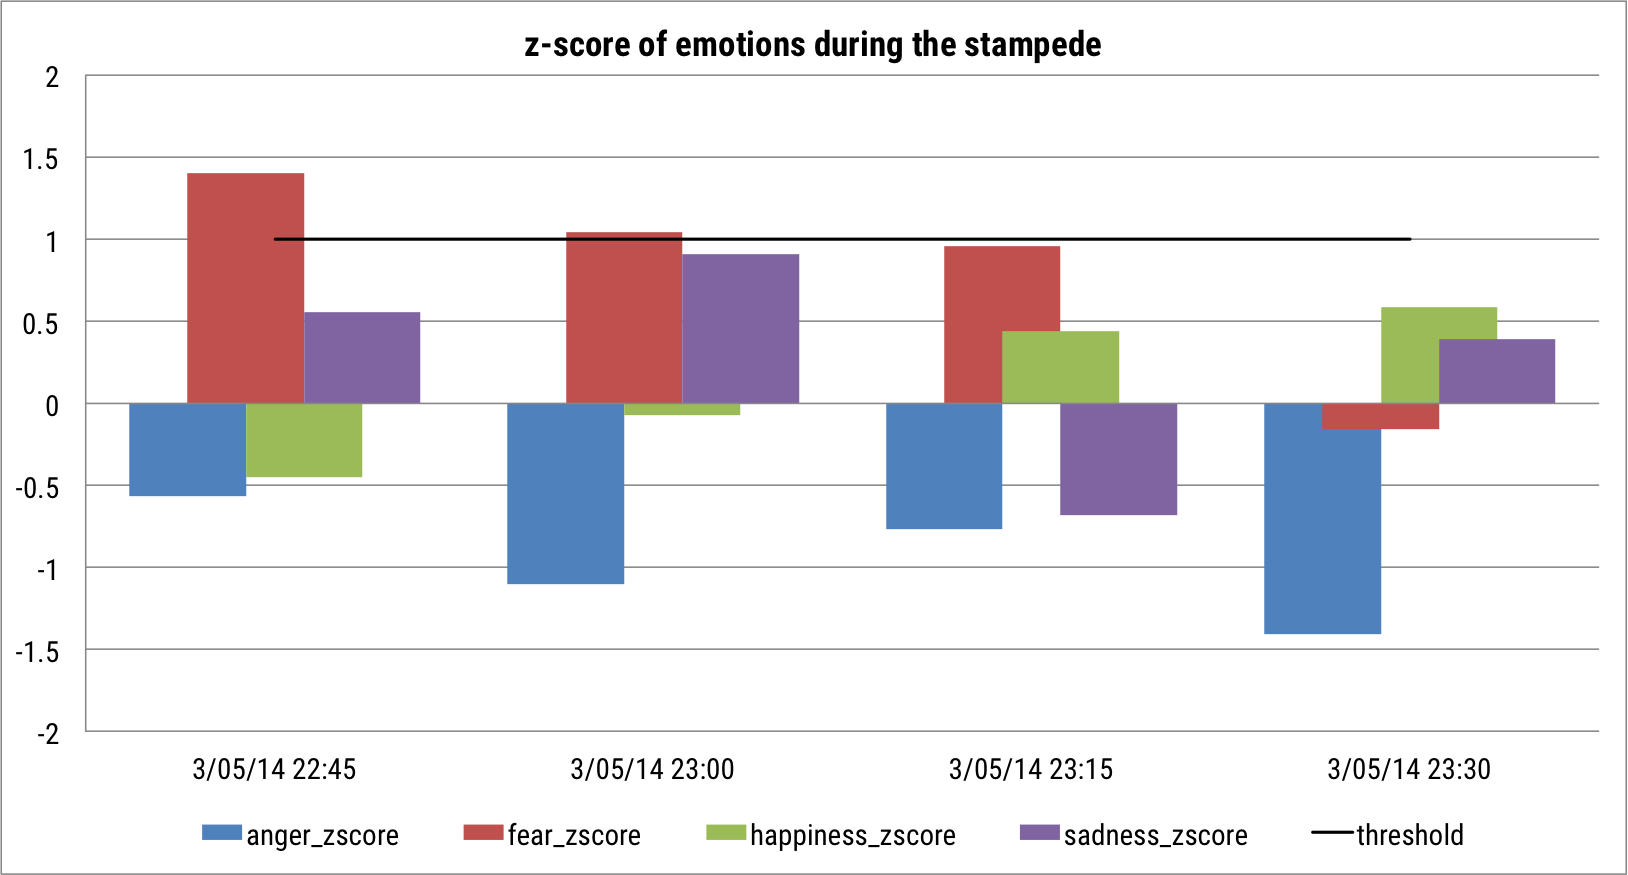
\includegraphics[width=1.0\textwidth]{EmotionZscoreFocus}
\caption{Threshold and z-score of emotions}
\label{fig:emotionZscoreFocus}
\end{figure}

Figure \ref{fig:emotionZscoreFocus} focuses on the one hour period when the stampede was happening. The threshold line represents our chosen high level threshold. It was noticeable that among four emotions, only \textit{fear} exceeded this threshold in two segments at 10:45PM and 11:00PM. It showed that when the stampede occurred there was a significant increase in the proportion of tweets labelled with \textit{fear}, suggesting a high level of fear in the crowd.

\subsubsection{Crowd Types Reasoning}
Figure \ref{fig:crowdTypeStampede} shows the result of the Rule Based Reasoning based on the levels of emotions. As can be seen, the inferred crowd types when the stampede occurred at 10:45PM stood out as the escaping crowd and the dense/suffocating crowd. These crowd types belong to Group 4 which is motivated by fear.

\begin{figure}[!htbp]
\centering
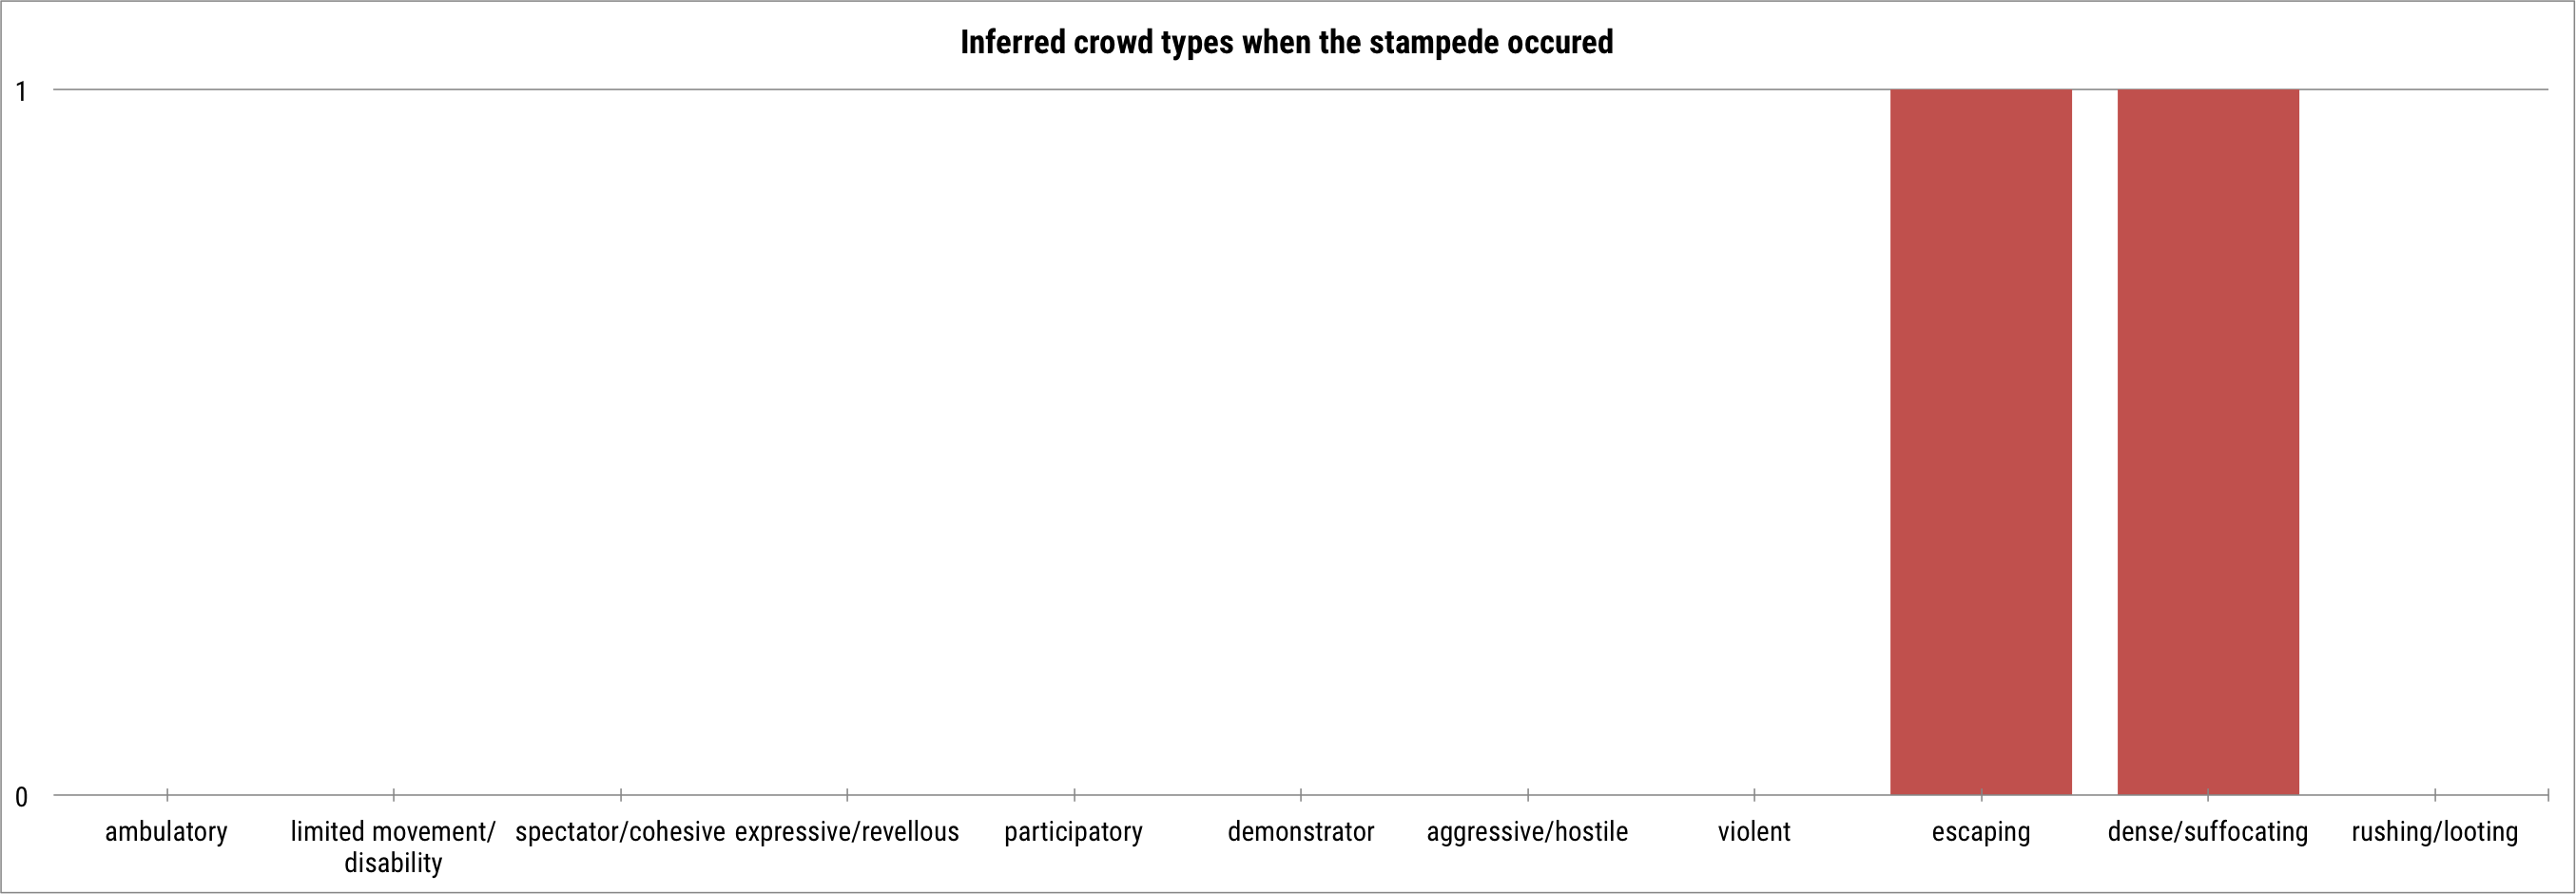
\includegraphics[width=0.75\textwidth]{CrowdTypeStampede}
\caption{Inferred crowd types where the stampede occurred}
\label{fig:crowdTypeStampede}
\end{figure}

\subsection{Discussion}

\subsubsection{Correctness and Timeliness of the Detection}
Firstly, regarding correctness of the detection, the inferred crowd types matched with the reported crowd types occurred the incident that were escaping and dense/suffocating crowd. Although our defined rules only lead to the group of crowd types rather than the exact crowd types, in this case study the rules were sufficient to point out a dangerous situation in the crowd.

In term of timeliness, using our proposed Emotion Analysis of the social media, the escaping crowd and dense/suffocating crowd were detected in the 10:45PM segment. It suggests that in a real-time monitoring, the result can be obtained the soonest at 11:00PM if the interval is selected as 15 minutes as in the experiment. According the official announcement, the local police received a phone call reporting about the stampede at 10:45PM, which was relatively close to our time of detection.

The case study has confirmed the capability of our proposed framework in term of producing correct and timely detection as soon as the stampede occurred. The collected data also brings forward questions and potential future researches which will be discussed in following sections.

\subsubsection{The shift in emotion during the event}
As mentioned earlier, tweets labelled with \textit{happiness} dominated the emotion distribution in the large sampling period of seven days. However, focusing on the data collected during the event, the number of tweets labelled with \textit{anger} surpassed that of \textit{happiness}. The reason for this shift in emotion might be due to the nature of the event which was a boxing match. The tweets related to a boxing match might contain words that associate to a certain degree of aggressiveness. This leads to the next question that whether the type of event has significant effect on the emotions of the people in the crowd or not, which will require further study.

\subsubsection{Behaviour in an emergency situation}
Another interesting discovery by further investigating collected data is context of tweets mentioning about the stampede when they were posted. It can be noticed that a large number of those tweets were not posted from the crowd. The first scenario is that the tweet was posted after the user safely got out of the crowd. It appears to be reasonable that during such an emergency situation, people would prioritise escaping over posting about it on social media. The second scenario is that the author of the tweet was not participating in the event and only reported about the incident. In this scenario, the author might be or not be influenced by the same emotion as the people in the crowd. Therefore, future researches are required to investigate further on the behaviour of people under emergency situation and the effect of emotion on people outside the crowd.

Table \ref{table:tweetStampede} extracts some tweets containing keyword ``stampede'' posted around the time of the incident. Most tweets seems to be posted under first scenario, while the last tweet belongs to the second scenario. Nevertheless, in our research both scenarios were able to offer information about the occurrence of the stampede, which was useful for our analysis to detect the emergency situation.

\begin{table}[!htb]
\centering
\caption{Sample tweets mentioning about the stampede}
\label{table:tweetStampede}
\begin{tabular}{|p{2.5cm}|p{12cm}|}

\hline
\textbf{Posted time} & \textbf{Tweet} \\ \hline \hline
2014-05-03 22:49:16 & A stampede of people just rushed into the media room a was very hectic Here at the MGM Grand \#TheMoment \#boxing \#boxeo \\ \hline
2014-05-03 22:53:00 & Was nearly trampled during a frightening stampede leaving MGM Grand Garden. Not the highlight of this trip. \#TheMoment \\ \hline
2014-05-03 23:15:05 & Crazy scenes @MGMGrand as shots were fired, we were caught in the stampede following the @floydmayweather flight. Many people injured. \\ \hline
2014-05-03 23:16:05 & Scary scenes at the MGM grand after the Mayweather fight apparently a gun was shot which caused a stampede plp crushed scary shit \\ \hline
2014-05-03 23:29:58 & Crazy fight, crazy night. Almost got trampled in a stampede outside the arena. Fights breaking out everywhere. Ugly atmosphere. \\ \hline
2014-05-03 23:57:46 & My friend just left the \#MayweatherMaidana fight @MGMGrand \& called to tell me she was scared but safe. \#stampede? \\ \hline
\end{tabular}
\end{table}

\subsubsection{Potential of Prediction}
Although crowd monitoring operation does not involve forecasting, the capability to predict an emergency situation will benefit the emergency management in the perspective of planning and preparation. Comparing the emotion rates of \textit{anger}, \textit{fear}, \textit{happiness} and \textit{sadness} before and after the occurrence of the stampede, an interesting pattern of change in emotion can be noticed. Figure \ref{fig:emotionRatePrediction} illustrates the emotion rate of the four emotions in two segments before and after the stampede occurred respectively. As can be seen, the emotion rate of \textit{happiness} dropped remarkably while the rates of the other three emotions rose. Because \textit{happiness} can be considered as a positive emotional state whereas \textit{anger}, \textit{fear} and \textit{sadness} have the negative tendency, this change in emotion might suggest a possible emergency situation.

\begin{figure}[!htbp]
\centering
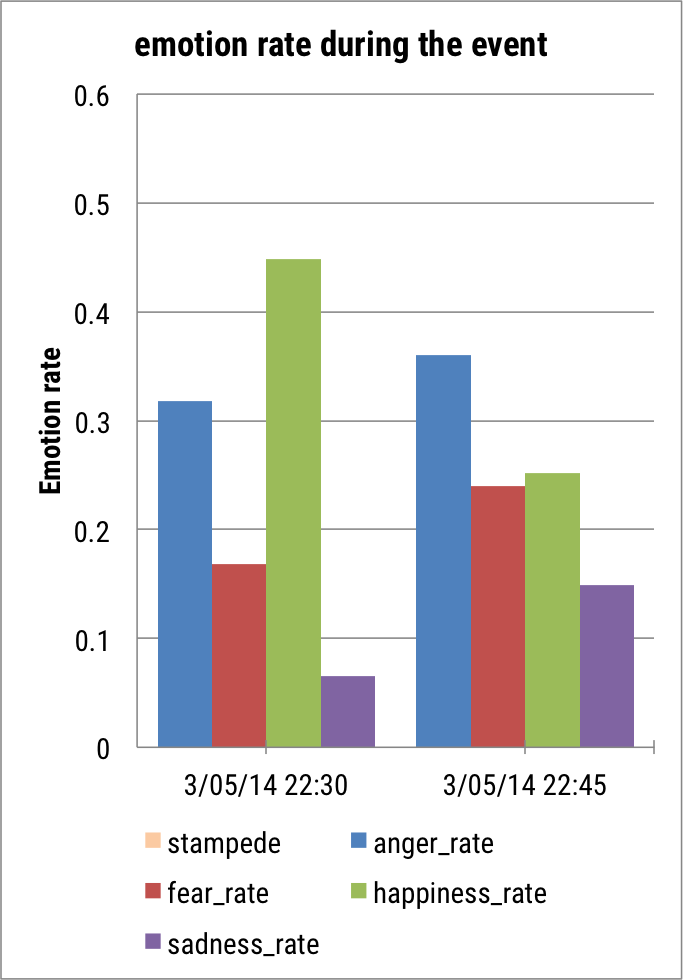
\includegraphics[width=0.4\textwidth]{EmotionRatePrediction}
\caption{Emotion rates of the four emotions before and after the occurrence of the stampede}
\label{fig:emotionRatePrediction}
\end{figure}

\section{Conclusion}
This chapter describes our evaluation of the proposed Crowd Monitoring Framework using a stampede accident occurred in a selected sporting event as a case study. A simple implementation to illustrate the framework's process has been introduced with moving average and z-score as the factors to determine the threshold for the high level of an emotion. The result of the experiment shows that using Emotion Analysis on the tweets collected about the event, the correct crowd types can be identified in a timely manner.
\chapter{Conclusion}

% **************************** Define Graphics Path **************************
\ifpdf
    \graphicspath{{Chapter6/Figs/Raster/}{Chapter6/Figs/PDF/}{Chapter6/Figs/}}
\else
    \graphicspath{{Chapter6/Figs/Vector/}{Chapter6/Figs/}}
\fi

\section{Introduction}
\section{Research Outcome}
\section{Future Research}
\subsection{Integrating Mobile Sensor Analysis}
Current only social media is integrated because of the limitation of the evaluation. Mobile sensors such as accelerometer or GPS can be used to collect contextual data and provide better crowd classification.

\subsection{Improvement of Emotion Classification}
Current use basic voting system. More advanced classification techniques can be used, such as SVM, neural network
\section{Conclusion}

% ********************************** Back Matter *******************************
% Backmatter should be commented out, if you are using appendices after References
%\backmatter

% ********************************** Bibliography ******************************
\begin{spacing}{0.9}

% To use the conventional natbib style referencing
% Bibliography style previews: http://nodonn.tipido.net/bibstyle.php
% Reference styles: http://sites.stat.psu.edu/~surajit/present/bib.htm

%\bibliographystyle{apalike}
%\bibliographystyle{plainnat} % use this to have URLs listed in References
\cleardoublepage
%\bibliography{References/references} % Path to your References.bib file


% If you would like to use BibLaTeX for your references, pass `custombib' as
% an option in the document class. The location of 'reference.bib' should be
% specified in the preamble.tex file in the custombib section.
% Comment out the lines related to natbib above and uncomment the following line.

\printbibliography[heading=bibintoc, title={References}]


\end{spacing}

% ********************************** Appendices ********************************

\begin{appendices} % Using appendices environment for more functunality

%% ******************************* Thesis Appendix A ********************************
\chapter{How to install \LaTeX} 

\section*{Windows OS}

\subsection*{TeXLive package - full version}
\begin{enumerate}
\item	Download the TeXLive ISO (2.2GB) from\\
\href{https://www.tug.org/texlive/}{https://www.tug.org/texlive/}
\item	Download WinCDEmu (if you don't have a virtual drive) from \\
\href{http://wincdemu.sysprogs.org/download/}{http://wincdemu.sysprogs.org/download/}
\item	To install Windows CD Emulator follow the instructions at\\
\href{http://wincdemu.sysprogs.org/tutorials/install/}{http://wincdemu.sysprogs.org/tutorials/install/}
\item	Right click the iso and mount it using the WinCDEmu as shown in \\
\href{http://wincdemu.sysprogs.org/tutorials/mount/}{http://wincdemu.sysprogs.org/tutorials/mount/}
\item	Open your virtual drive and run setup.pl
\end{enumerate}

or

\subsection*{Basic MikTeX - TeX distribution}
\begin{enumerate}
\item	Download Basic-MiK\TeX (32bit or 64bit) from\\
\href{http://miktex.org/download}{http://miktex.org/download}
\item	Run the installer 
\item	To add a new package go to Start >> All Programs >> MikTex >> Maintenance (Admin) and choose Package Manager
\item	Select or search for packages to install
\end{enumerate}

\subsection*{TexStudio - Tex Editor}
\begin{enumerate}
\item	Download TexStudio from\\
\href{http://texstudio.sourceforge.net/\#downloads}{http://texstudio.sourceforge.net/\#downloads} 
\item	Run the installer
\end{enumerate}

\section*{Mac OS X}
\subsection*{MacTeX - TeX distribution}
\begin{enumerate}
\item	Download the file from\\
\href{https://www.tug.org/mactex/}{https://www.tug.org/mactex/}
\item	Extract and double click to run the installer. It does the entire configuration, sit back and relax.
\end{enumerate}

\subsection*{TexStudio - Tex Editor}
\begin{enumerate}
\item	Download TexStudio from\\
\href{http://texstudio.sourceforge.net/\#downloads}{http://texstudio.sourceforge.net/\#downloads} 
\item	Extract and Start
\end{enumerate}


\section*{Unix/Linux}
\subsection*{TeXLive - TeX distribution}
\subsubsection*{Getting the distribution:}
\begin{enumerate}
\item	TexLive can be downloaded from\\
\href{http://www.tug.org/texlive/acquire-netinstall.html}{http://www.tug.org/texlive/acquire-netinstall.html}.
\item	TexLive is provided by most operating system you can use (rpm,apt-get or yum) to get TexLive distributions
\end{enumerate}

\subsubsection*{Installation}
\begin{enumerate}
\item	Mount the ISO file in the mnt directory
\begin{verbatim}
mount -t iso9660 -o ro,loop,noauto /your/texlive####.iso /mnt
\end{verbatim}

\item	Install wget on your OS (use rpm, apt-get or yum install)
\item	Run the installer script install-tl.
\begin{verbatim}
	cd /your/download/directory
	./install-tl
\end{verbatim}
\item	Enter command `i' for installation

\item	Post-Installation configuration:\\
\href{http://www.tug.org/texlive/doc/texlive-en/texlive-en.html\#x1-320003.4.1}{http://www.tug.org/texlive/doc/texlive-en/texlive-en.html\#x1-320003.4.1} 
\item	Set the path for the directory of TexLive binaries in your .bashrc file
\end{enumerate}

\subsubsection*{For 32Bit OS}
For Bourne-compatible shells such as bash, and using Intel x86 GNU/Linux and a default directory setup as an example, the file to edit might be \begin{verbatim}
edit $~/.bashrc file and add following lines
PATH=/usr/local/texlive/2011/bin/i386-linux:$PATH; 
export PATH 
MANPATH=/usr/local/texlive/2011/texmf/doc/man:$MANPATH;
export MANPATH 
INFOPATH=/usr/local/texlive/2011/texmf/doc/info:$INFOPATH;
export INFOPATH
\end{verbatim}
\subsubsection*{For 64Bit}
\begin{verbatim}
edit $~/.bashrc file and add following lines
PATH=/usr/local/texlive/2011/bin/x86_64-linux:$PATH;
export PATH 
MANPATH=/usr/local/texlive/2011/texmf/doc/man:$MANPATH;
export MANPATH 
INFOPATH=/usr/local/texlive/2011/texmf/doc/info:$INFOPATH;
export INFOPATH

\end{verbatim}



%\subsection{Installing directly using Linux packages} 
\subsubsection*{Fedora/RedHat/CENTOS:}
\begin{verbatim} 
sudo yum install texlive 
sudo yum install psutils 
\end{verbatim}


\subsubsection*{SUSE:}
\begin{verbatim}
sudo zypper install texlive
\end{verbatim}


\subsubsection*{Debian/Ubuntu:}
\begin{verbatim} 
sudo apt-get install texlive texlive-latex-extra 
sudo apt-get install psutils
\end{verbatim}


\end{appendices}

% *************************************** Index ********************************
\printthesisindex % If index is present

\end{document}
